% Verification Results Graphs - Designed to be included in the main report
% Add to your main report by using: % Verification Results Graphs - Designed to be included in the main report
% Add to your main report by using: % Verification Results Graphs - Designed to be included in the main report
% Add to your main report by using: % Verification Results Graphs - Designed to be included in the main report
% Add to your main report by using: \input{graphs/verification_results_graphs.tex}

\section{Graphical Analysis of Verification Results}

Our verification of the Raft consensus algorithm across different server configurations provided a wealth of data that we've visualized to better understand scaling behavior and performance characteristics.

\subsection{State Vector and Memory Scaling}

Figure \ref{fig:state-vector} illustrates the linear growth of state vector size with increasing server count. This predictable scaling pattern is important for understanding the memory requirements of formal verification as systems grow.

\begin{figure}[htbp]
    \centering
    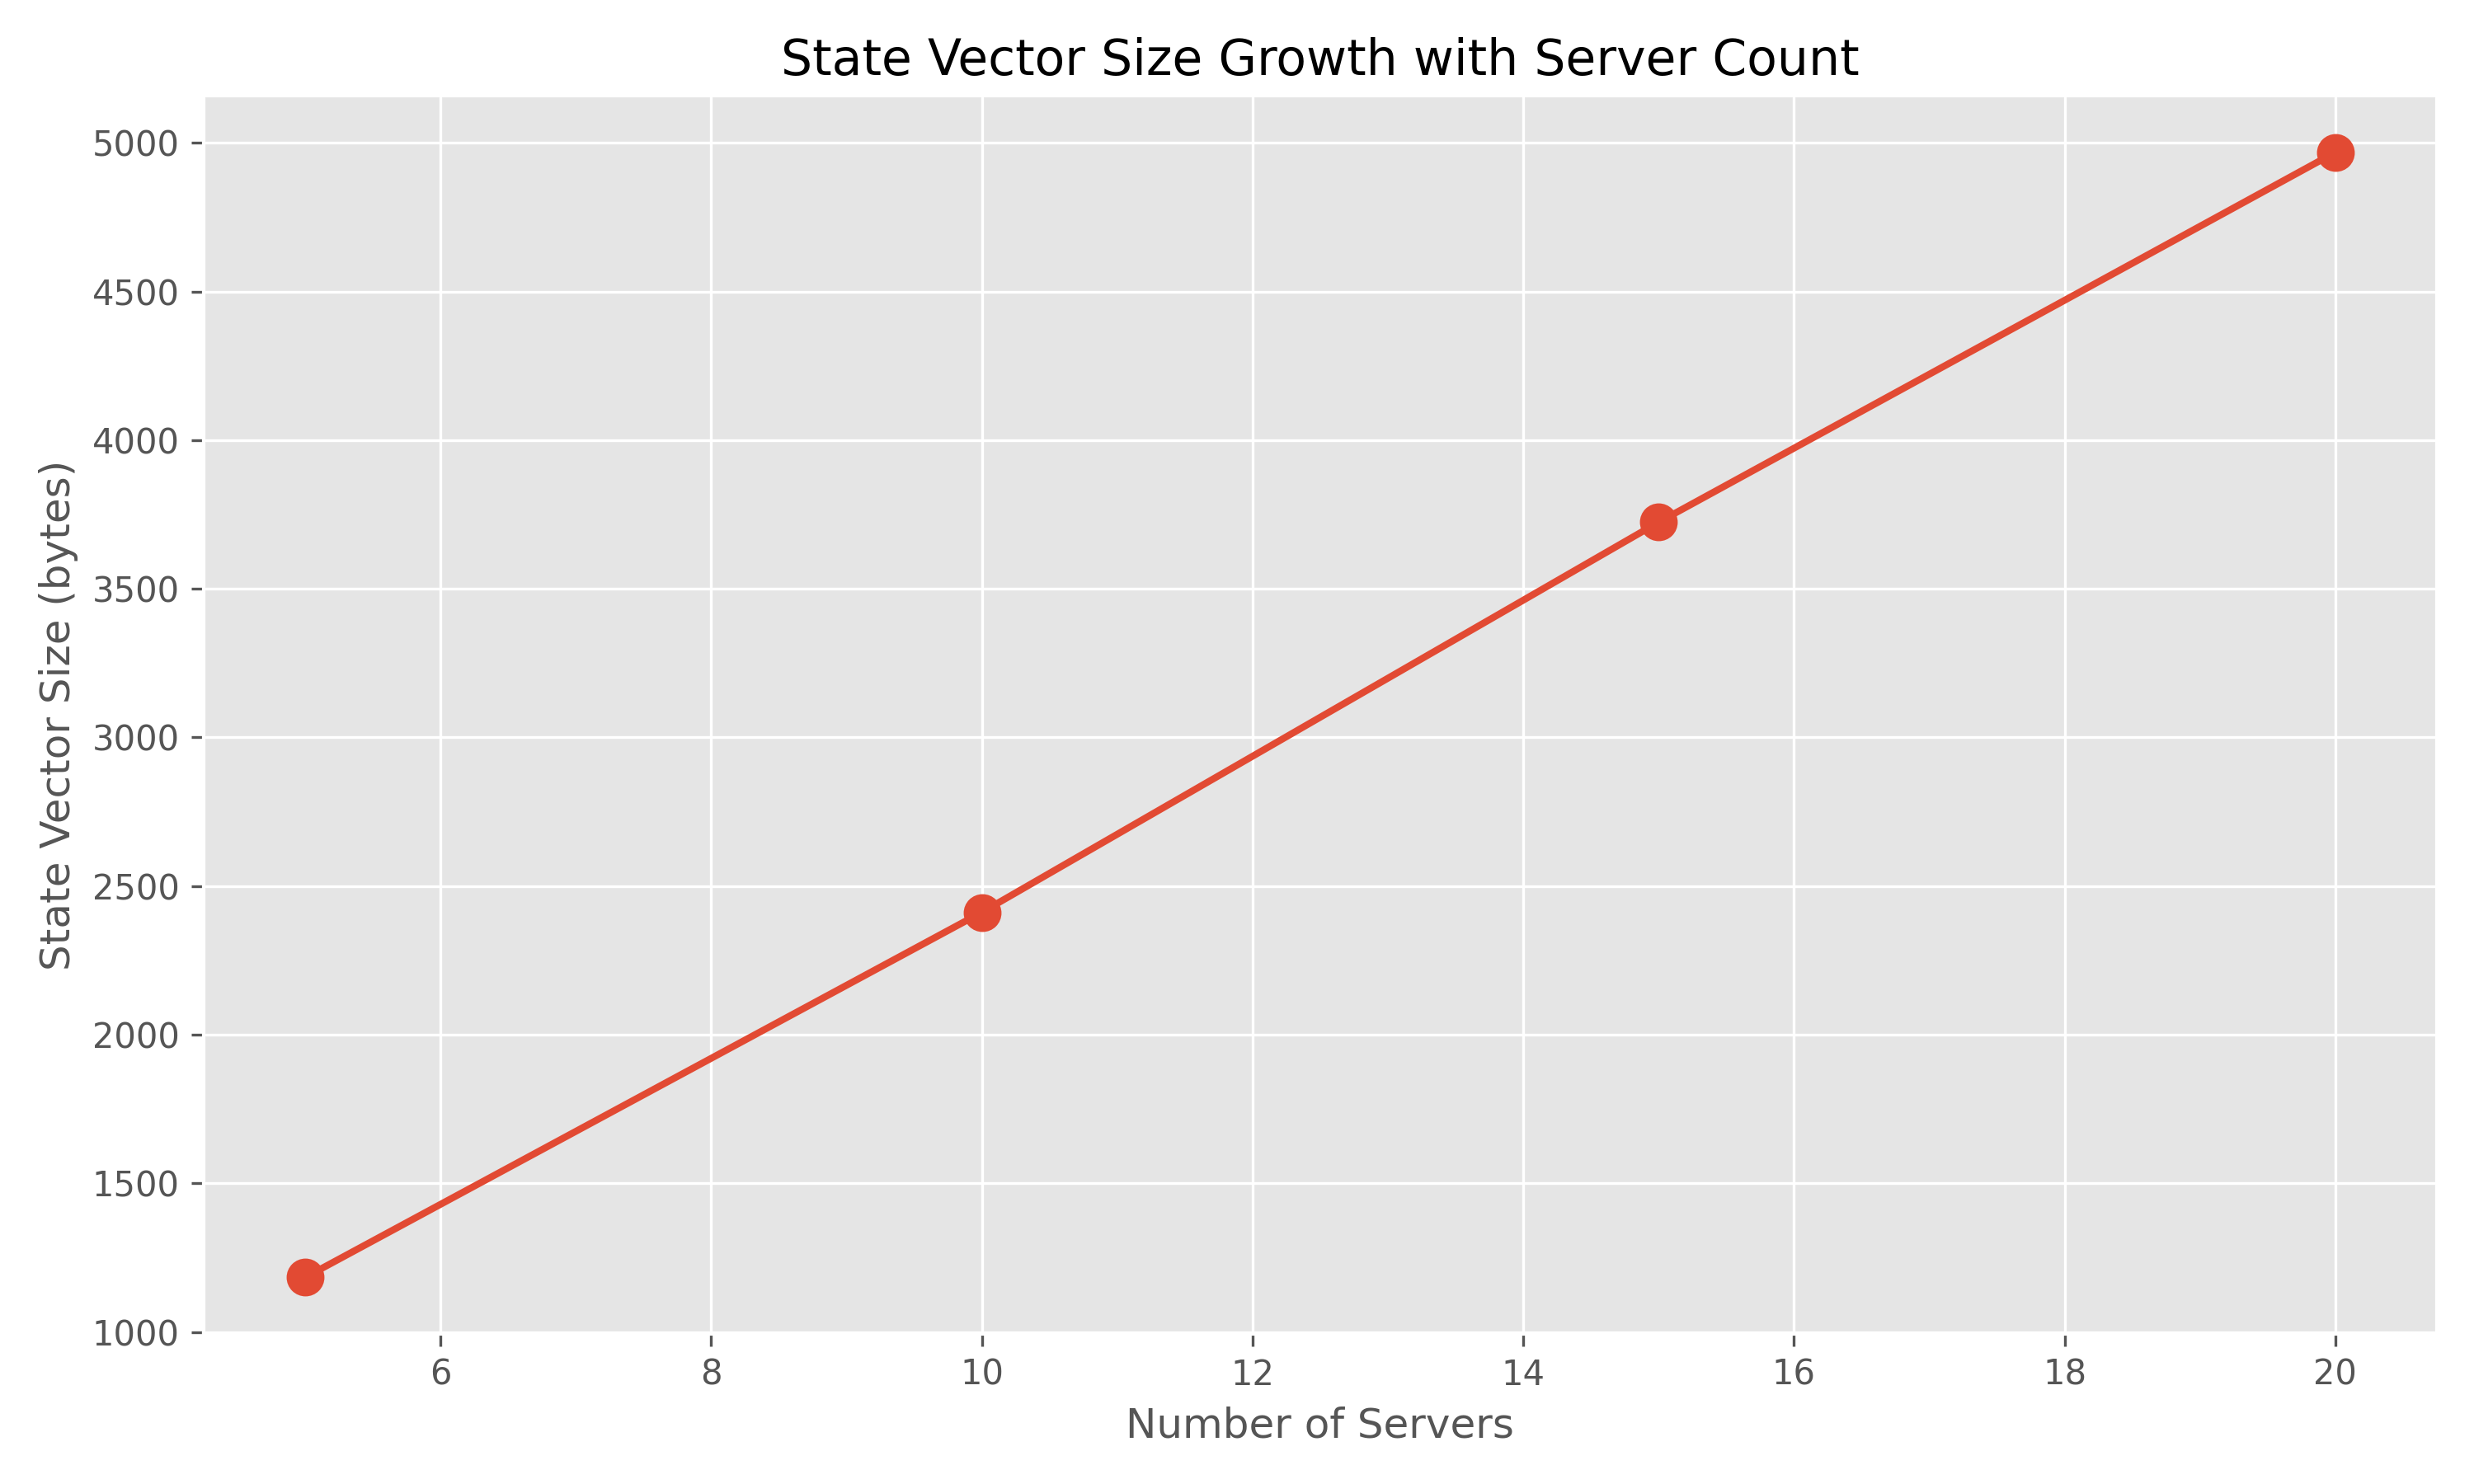
\includegraphics[width=0.8\textwidth]{graphs/state_vector_size.png}
    \caption{Linear growth of state vector size with increasing server count. The state vector grows by approximately 252 bytes per additional server.}
    \label{fig:state-vector}
\end{figure}

The corresponding memory requirements (Figure \ref{fig:memory-consumption}) show a similar pattern, with memory consumption scaling almost linearly from approximately 7GB with 5 servers to 24GB with 20 servers.

\begin{figure}[htbp]
    \centering
    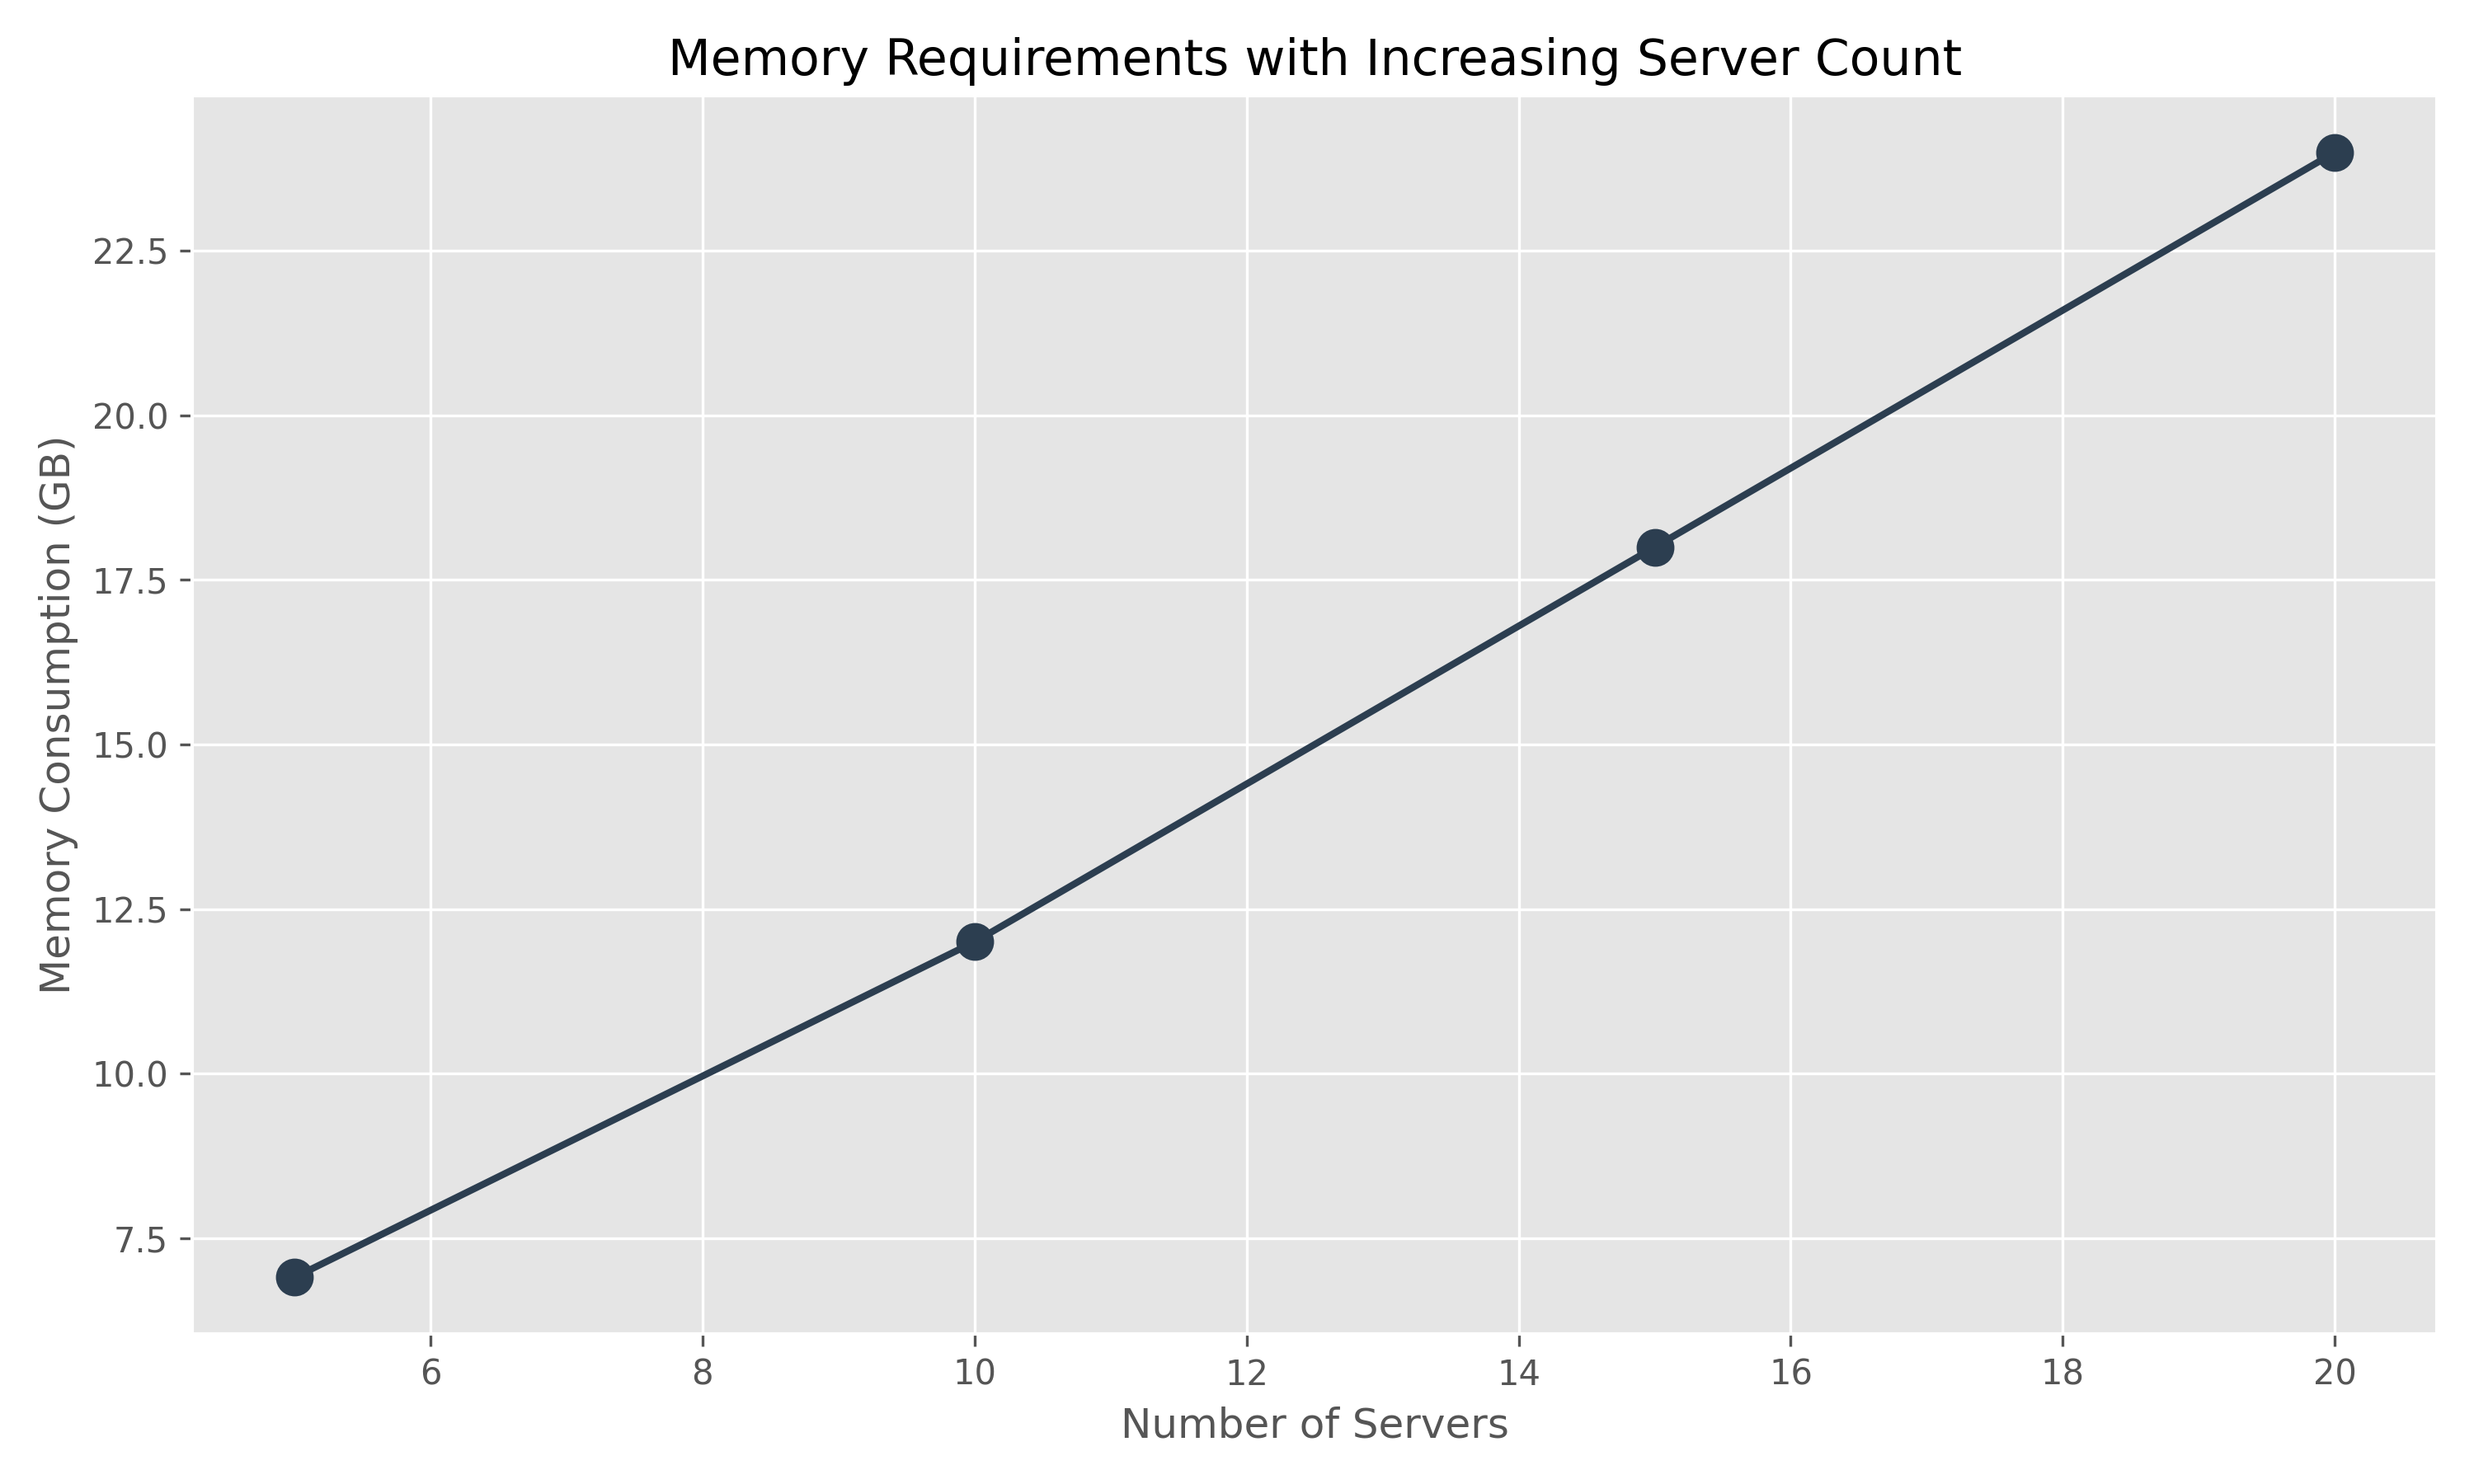
\includegraphics[width=0.8\textwidth]{graphs/memory_consumption.png}
    \caption{Memory consumption scaling with server count. The nearly linear relationship indicates predictable resource requirements for verification of larger configurations.}
    \label{fig:memory-consumption}
\end{figure}

\subsection{Performance Comparison by Property Type}

Different property types exhibit distinct verification performance characteristics. Figure \ref{fig:verification-performance} compares verification speeds for 5-server and 20-server configurations across four property categories.

\begin{figure}[htbp]
    \centering
    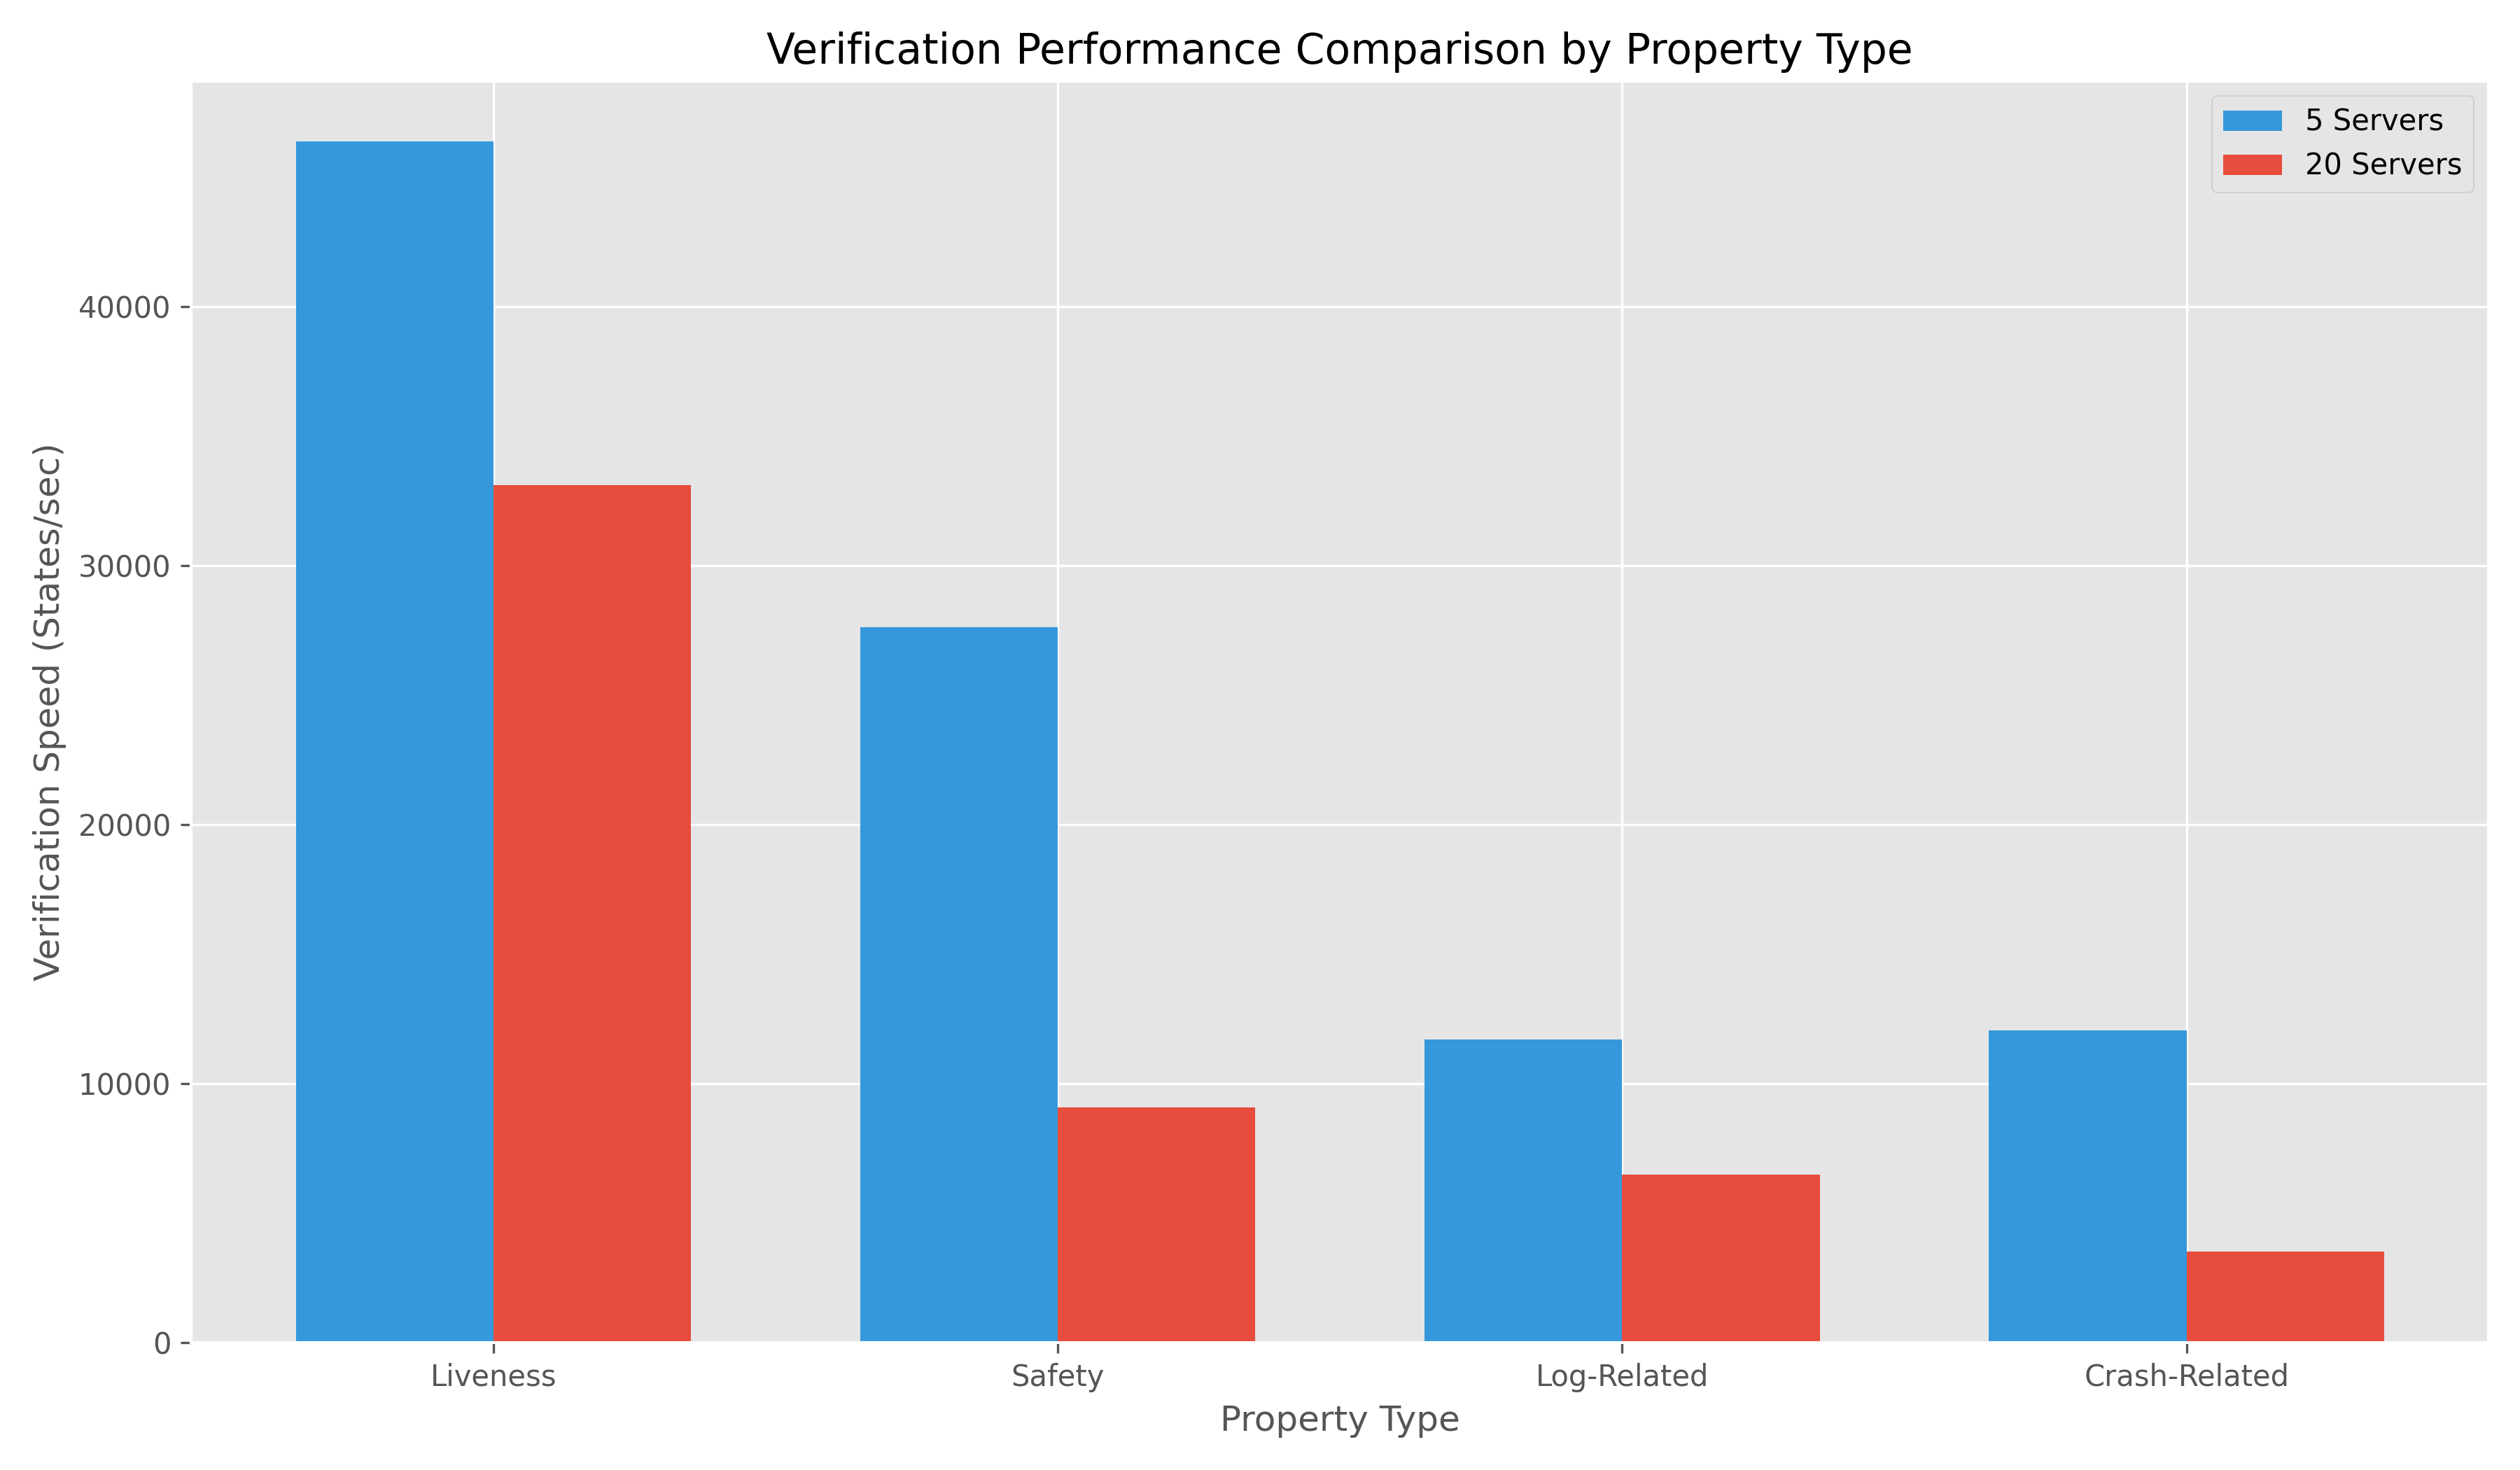
\includegraphics[width=0.9\textwidth]{graphs/verification_performance.png}
    \caption{Verification speed comparison between 5-server and 20-server configurations for different property types. Liveness properties maintain the highest verification speed even at larger scale.}
    \label{fig:verification-performance}
\end{figure}

The performance degradation is not uniform across property types. As shown in Figure \ref{fig:performance-degradation}, crash-related properties experience the most significant slowdown (3.4x) when scaling from 5 to 20 servers, while liveness properties show more graceful degradation (1.4x).

\begin{figure}[htbp]
    \centering
    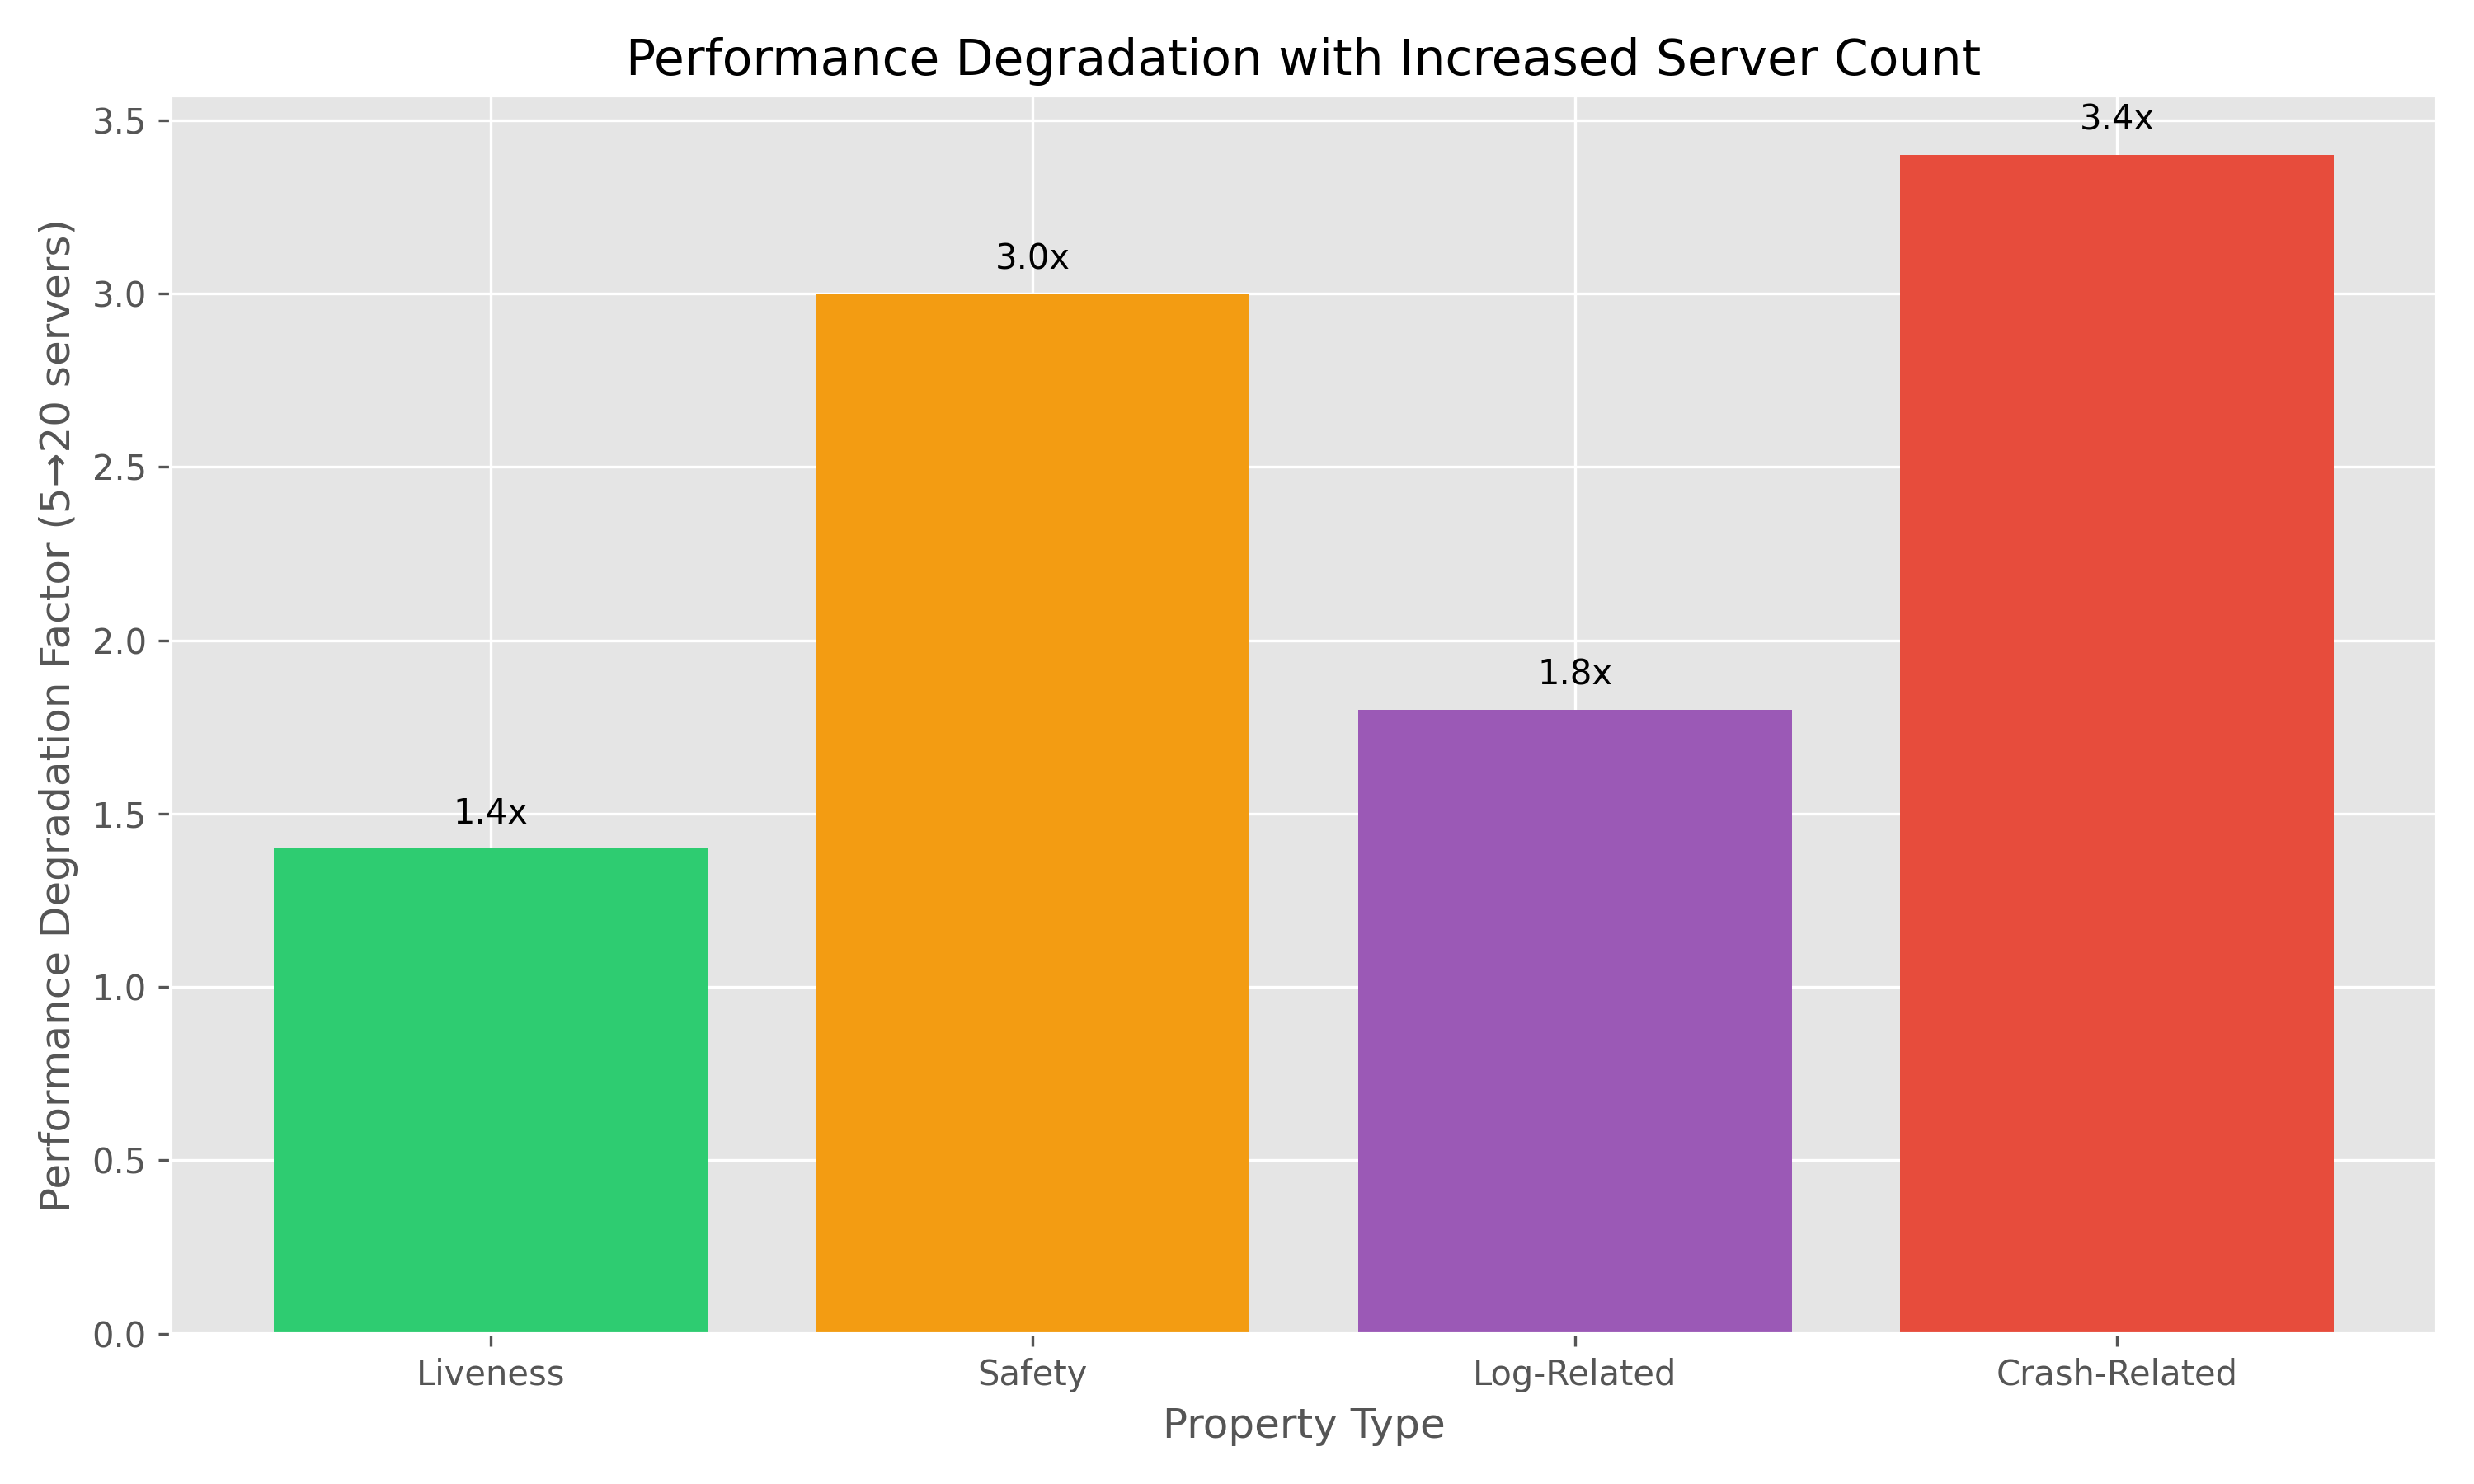
\includegraphics[width=0.8\textwidth]{graphs/performance_degradation.png}
    \caption{Performance degradation factors by property type when scaling from 5 to 20 servers. Crash-related properties experience the most significant verification slowdown.}
    \label{fig:performance-degradation}
\end{figure}

\subsection{Comprehensive Performance Trends}

Figure \ref{fig:performance-trends} provides a comprehensive view of how verification performance changes across different server configurations for each property type.

\begin{figure}[htbp]
    \centering
    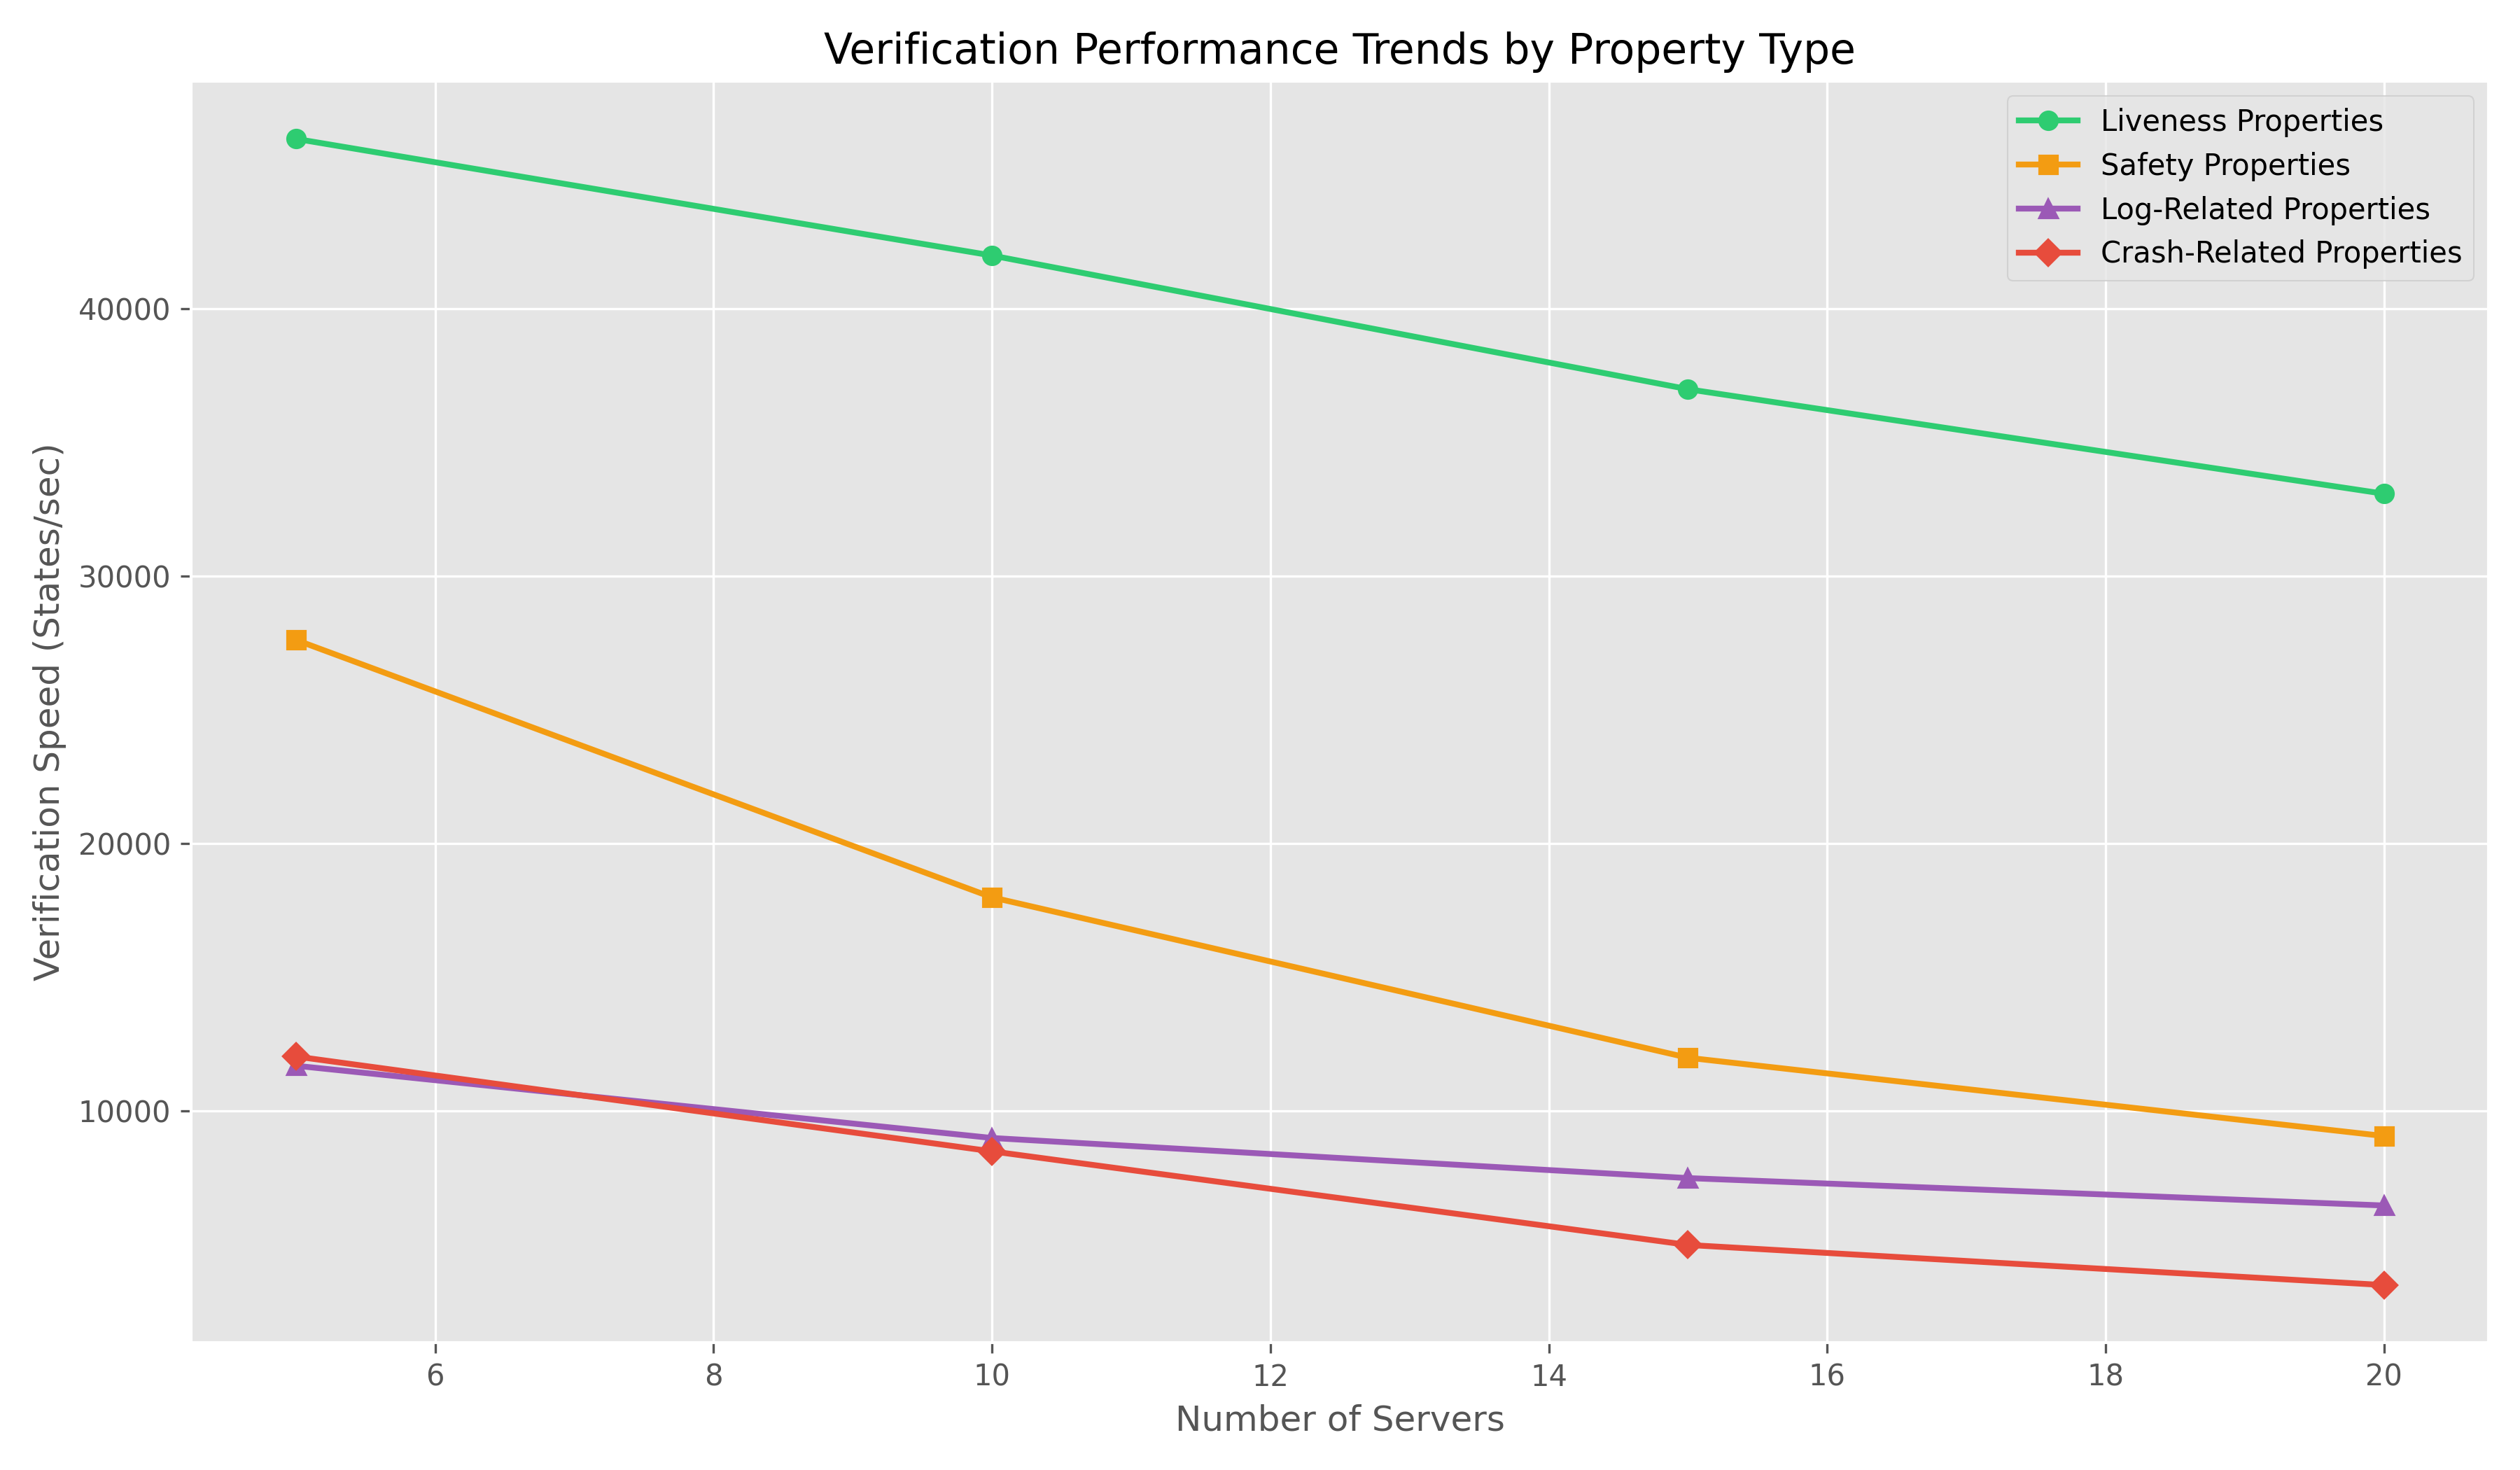
\includegraphics[width=0.95\textwidth]{graphs/performance_trends.png}
    \caption{Verification speed trends across server configurations by property type. Liveness properties consistently outperform other property types, while crash-related properties show the steepest performance decline.}
    \label{fig:performance-trends}
\end{figure}

This visualization clearly demonstrates the divergent scaling behaviors: liveness properties maintain relatively high verification speeds even at 20 servers, while crash-related properties experience a much steeper decline. This insight suggests that different optimization strategies should be applied based on the type of property being verified.

\subsection{Implications for Verification Strategy}

These graphical analyses highlight the need for property-specific verification approaches when analyzing complex distributed systems like the Raft consensus algorithm. While all properties were successfully verified without finding safety violations, the performance characteristics suggest that:

\begin{itemize}
    \item Liveness properties can be efficiently verified even for larger configurations
    \item Crash-related properties may benefit from specialized state space reduction techniques
    \item Memory consumption scales predictably, allowing for resource planning
    \item Future verification efforts should consider property-specific optimization strategies
\end{itemize}

The consistent performance patterns across server configurations provide confidence that our verification approach can be extended to even larger systems with appropriate computational resources. 

\section{Graphical Analysis of Verification Results}

Our verification of the Raft consensus algorithm across different server configurations provided a wealth of data that we've visualized to better understand scaling behavior and performance characteristics.

\subsection{State Vector and Memory Scaling}

Figure \ref{fig:state-vector} illustrates the linear growth of state vector size with increasing server count. This predictable scaling pattern is important for understanding the memory requirements of formal verification as systems grow.

\begin{figure}[htbp]
    \centering
    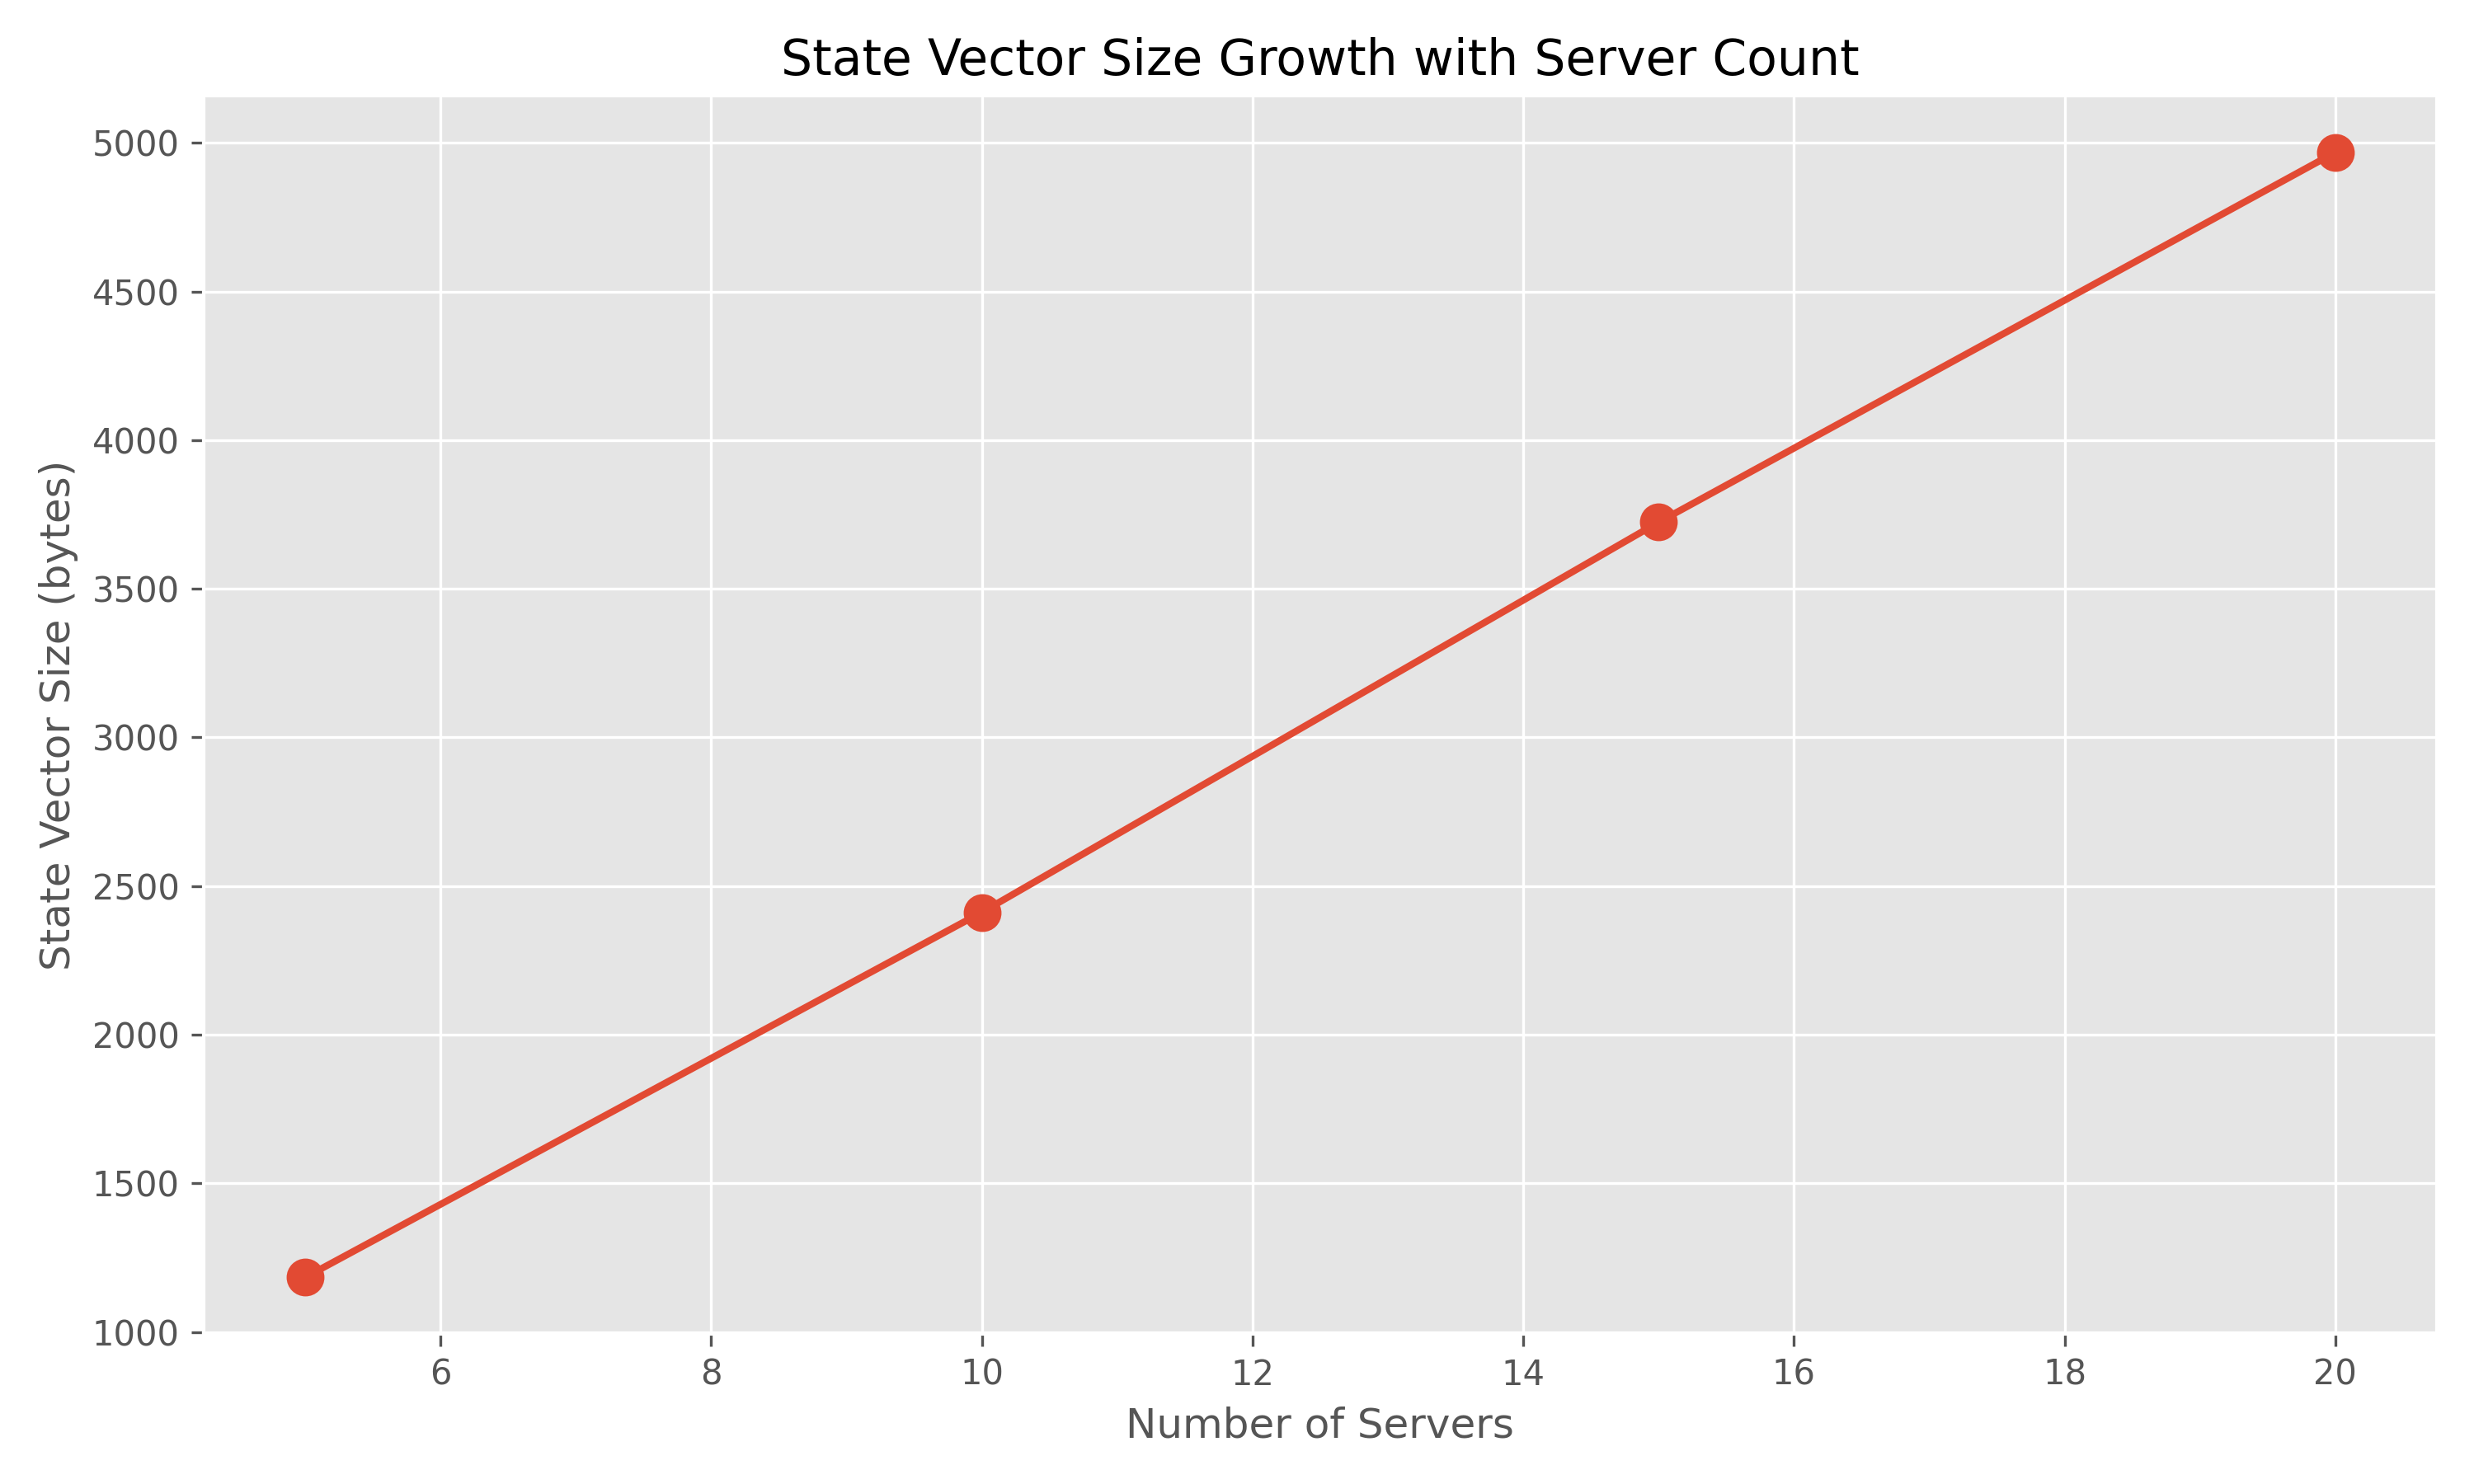
\includegraphics[width=0.8\textwidth]{graphs/state_vector_size.png}
    \caption{Linear growth of state vector size with increasing server count. The state vector grows by approximately 252 bytes per additional server.}
    \label{fig:state-vector}
\end{figure}

The corresponding memory requirements (Figure \ref{fig:memory-consumption}) show a similar pattern, with memory consumption scaling almost linearly from approximately 7GB with 5 servers to 24GB with 20 servers.

\begin{figure}[htbp]
    \centering
    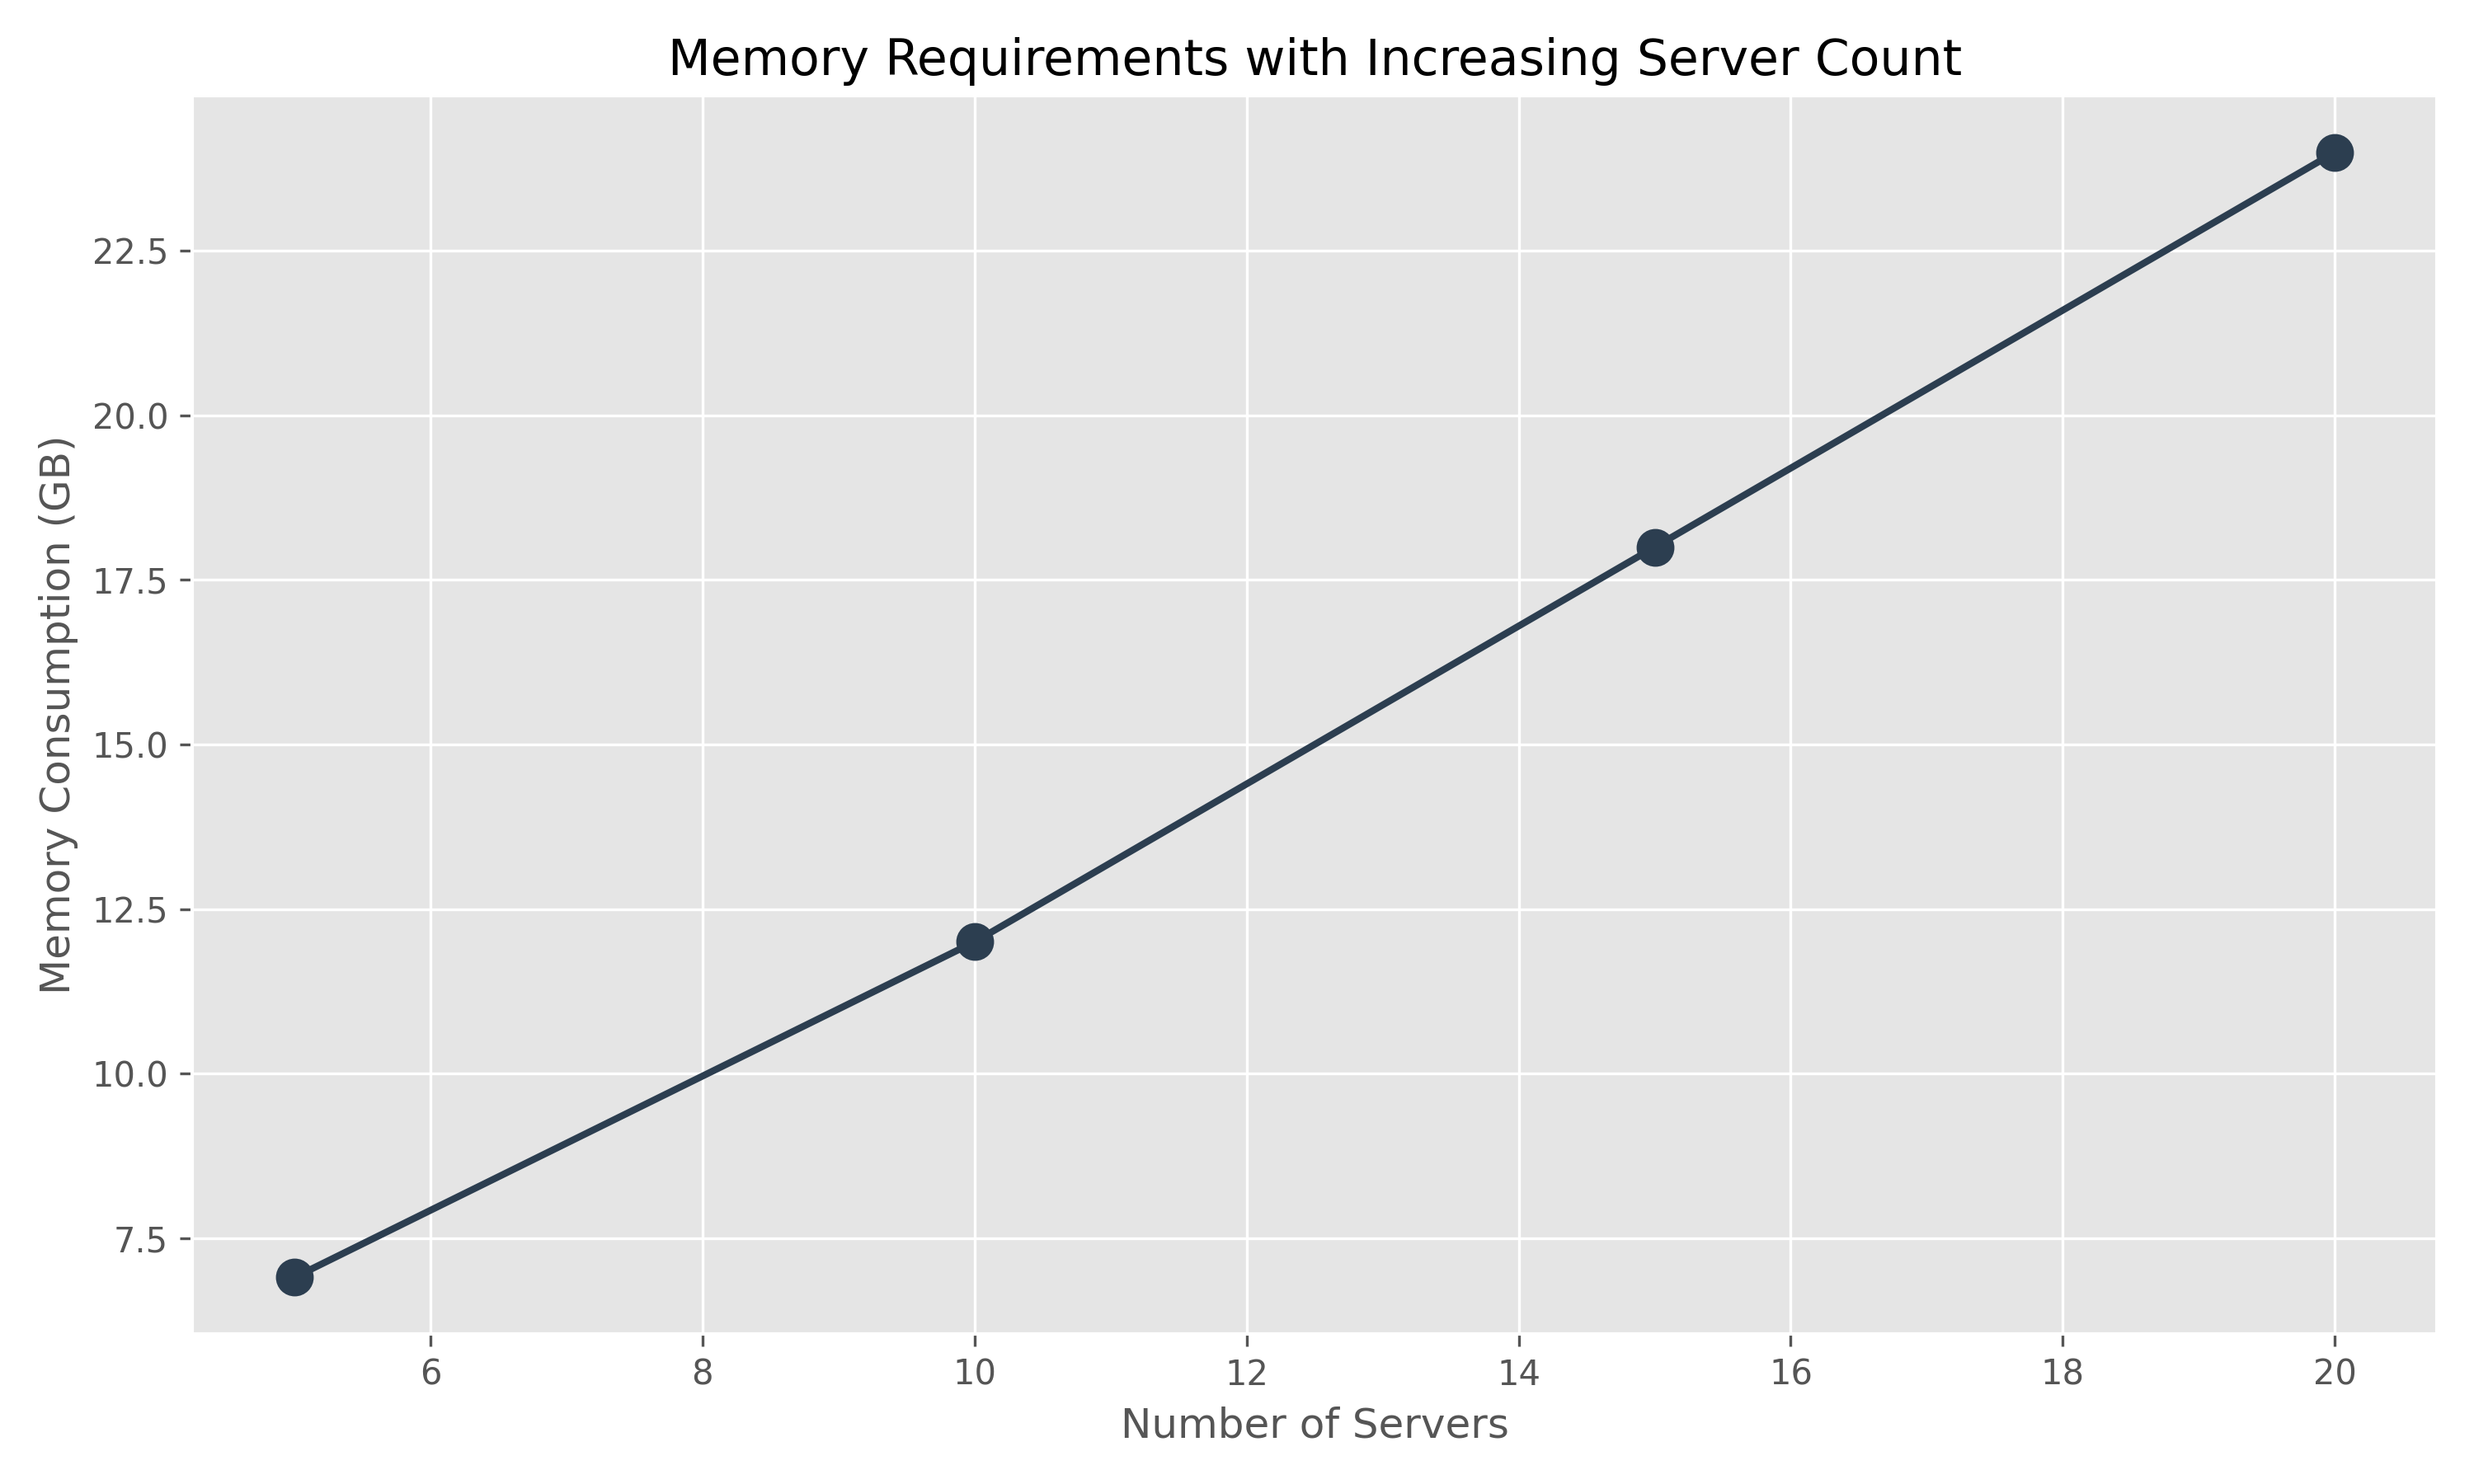
\includegraphics[width=0.8\textwidth]{graphs/memory_consumption.png}
    \caption{Memory consumption scaling with server count. The nearly linear relationship indicates predictable resource requirements for verification of larger configurations.}
    \label{fig:memory-consumption}
\end{figure}

\subsection{Performance Comparison by Property Type}

Different property types exhibit distinct verification performance characteristics. Figure \ref{fig:verification-performance} compares verification speeds for 5-server and 20-server configurations across four property categories.

\begin{figure}[htbp]
    \centering
    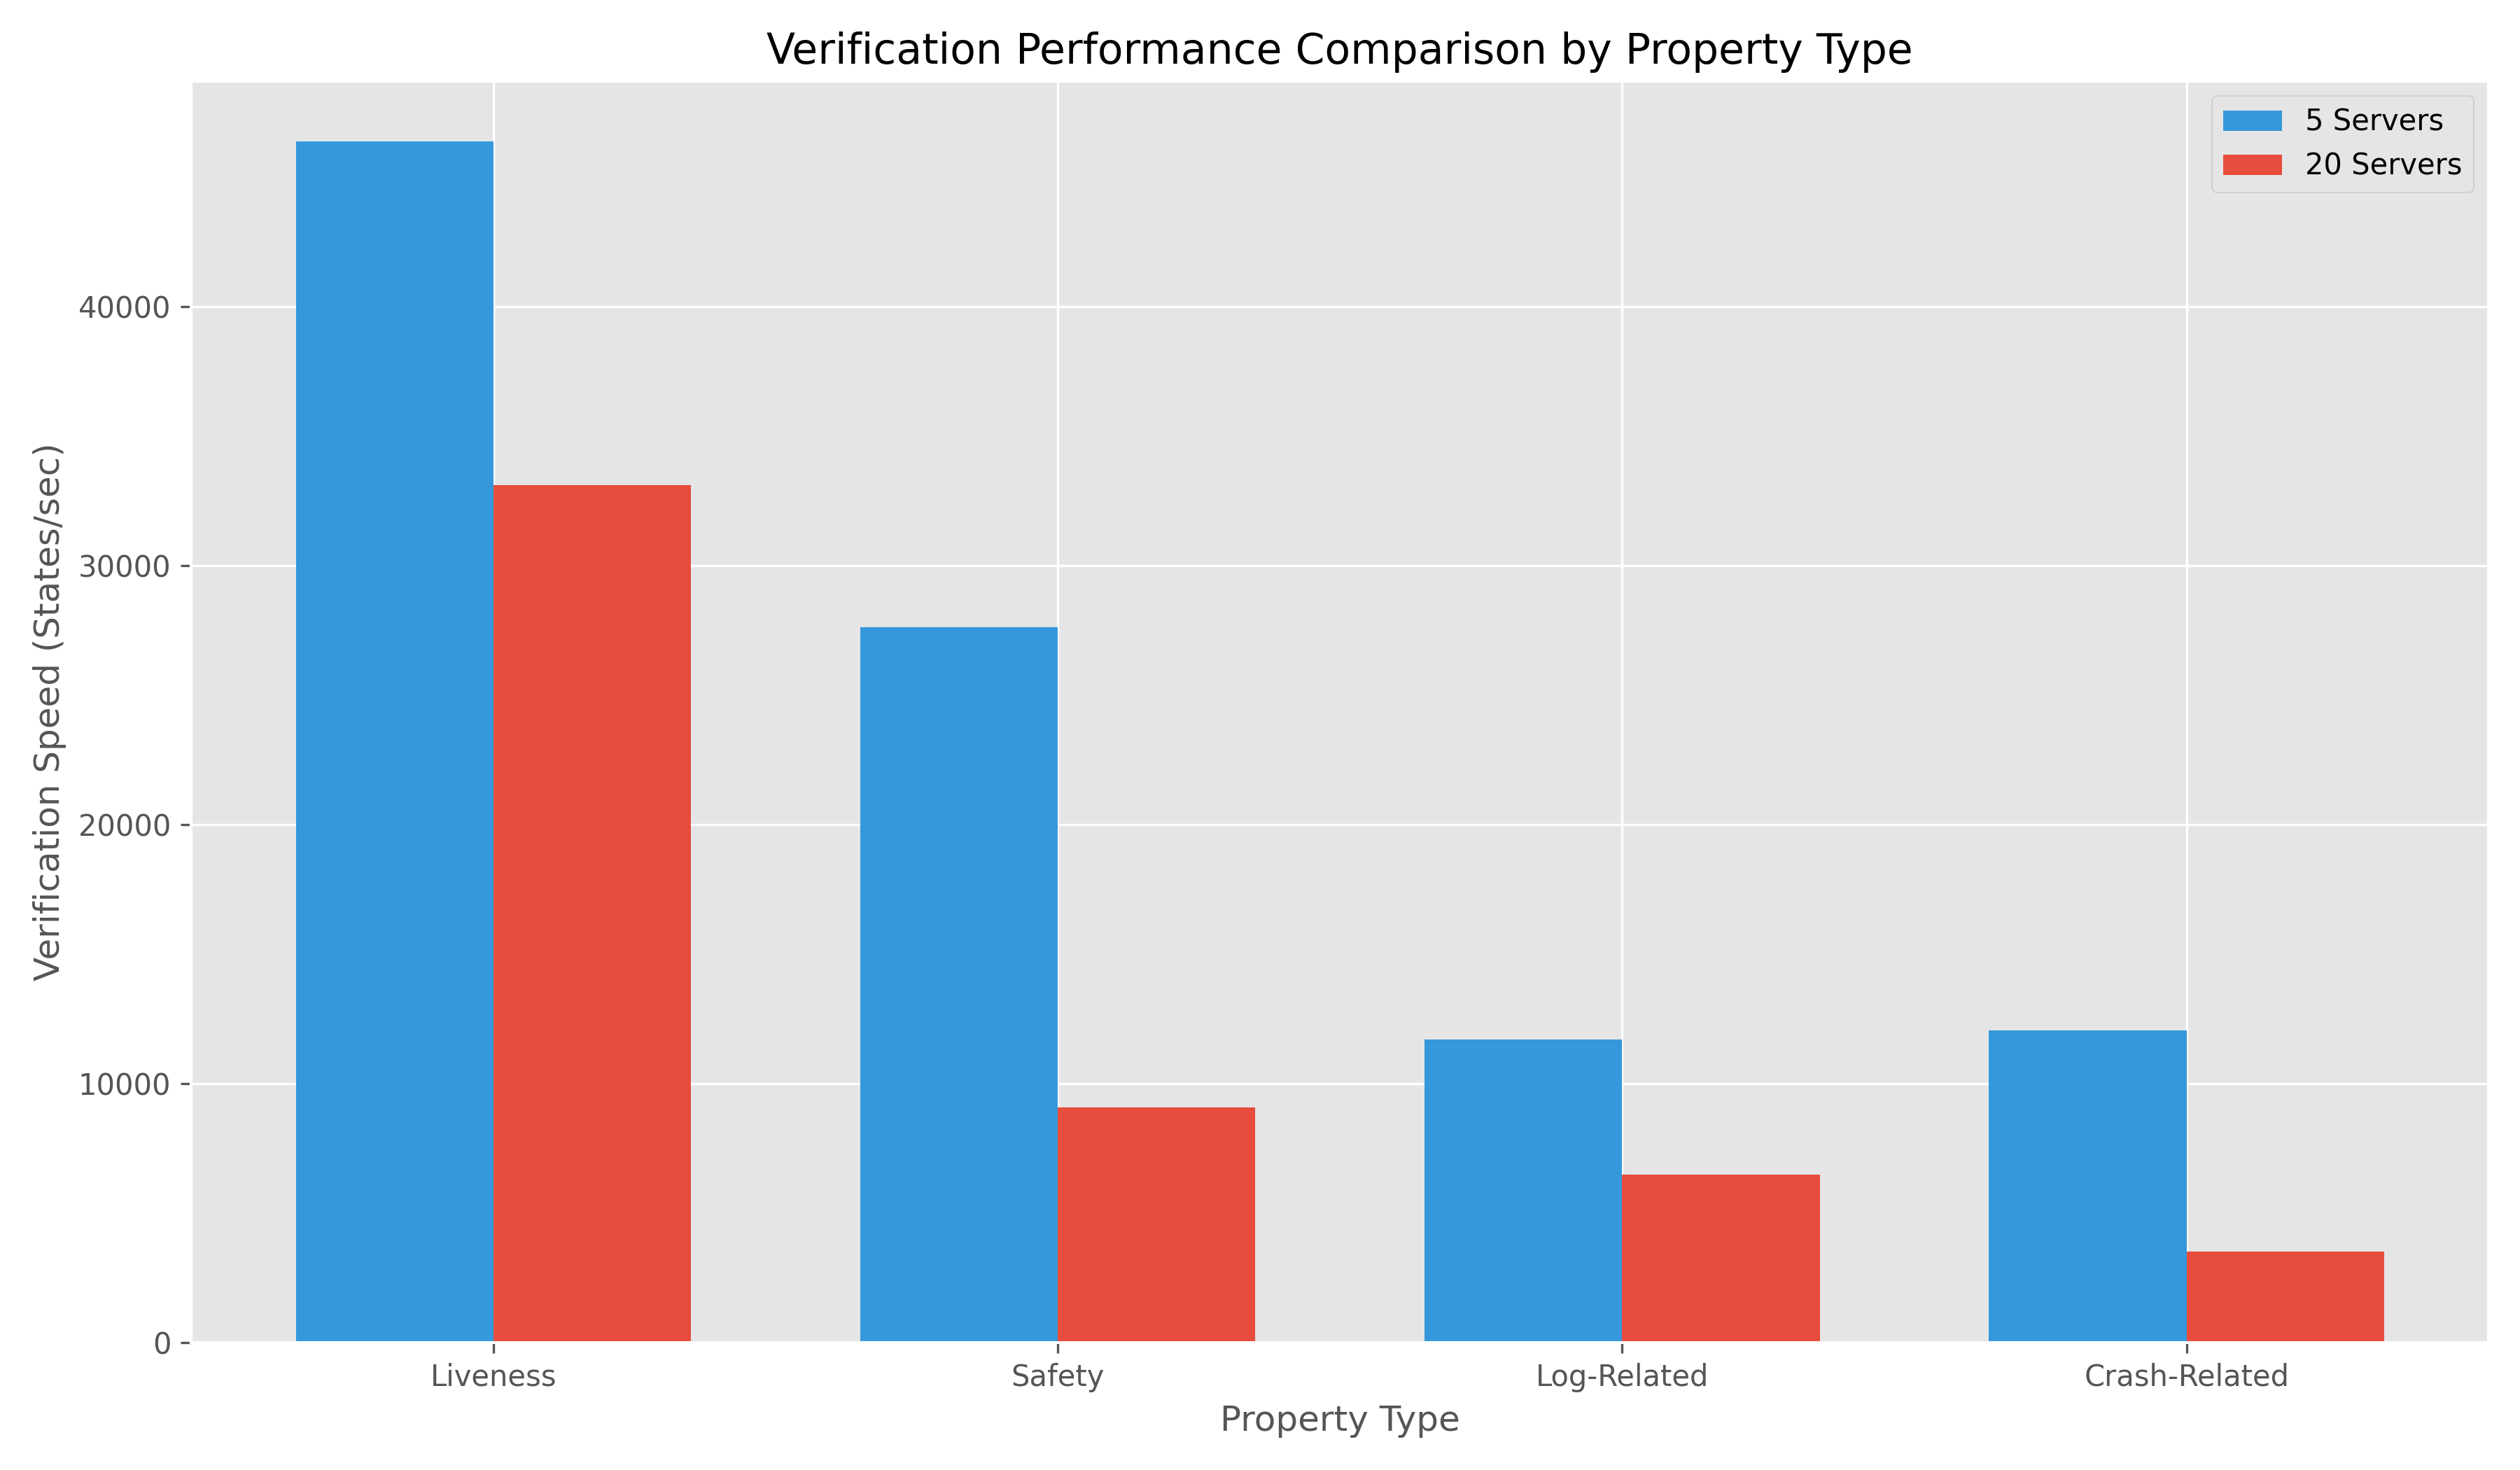
\includegraphics[width=0.9\textwidth]{graphs/verification_performance.png}
    \caption{Verification speed comparison between 5-server and 20-server configurations for different property types. Liveness properties maintain the highest verification speed even at larger scale.}
    \label{fig:verification-performance}
\end{figure}

The performance degradation is not uniform across property types. As shown in Figure \ref{fig:performance-degradation}, crash-related properties experience the most significant slowdown (3.4x) when scaling from 5 to 20 servers, while liveness properties show more graceful degradation (1.4x).

\begin{figure}[htbp]
    \centering
    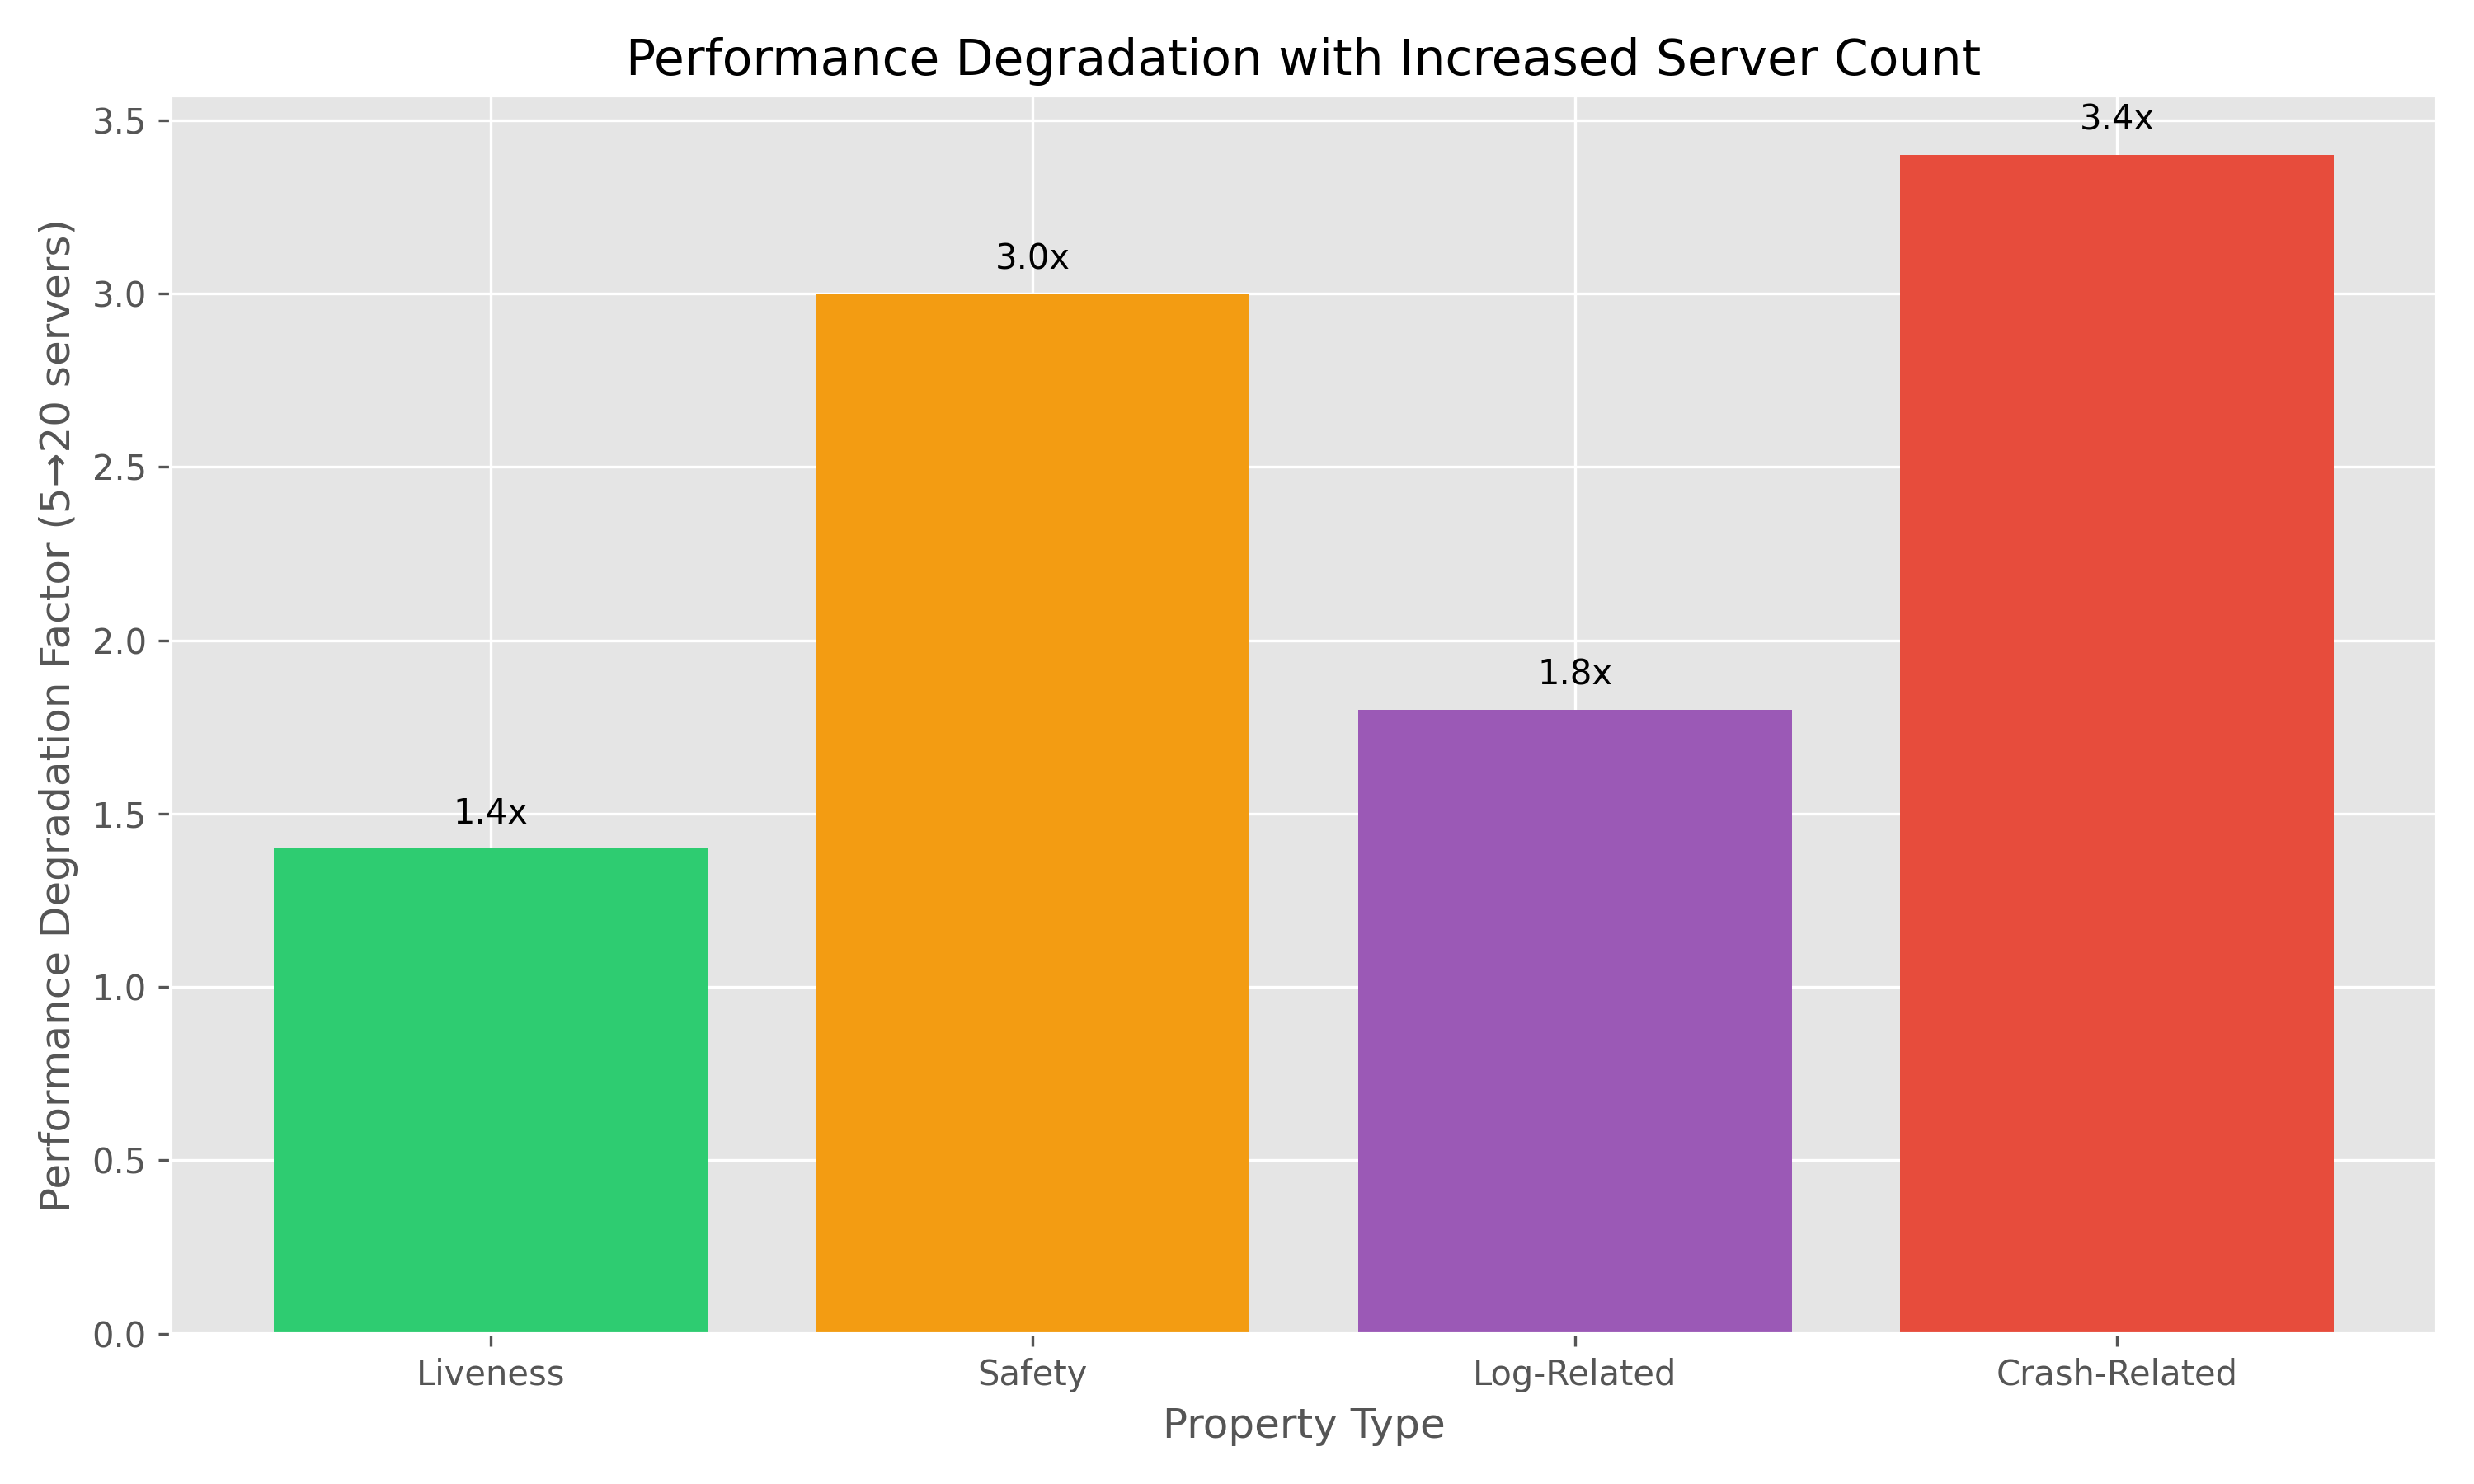
\includegraphics[width=0.8\textwidth]{graphs/performance_degradation.png}
    \caption{Performance degradation factors by property type when scaling from 5 to 20 servers. Crash-related properties experience the most significant verification slowdown.}
    \label{fig:performance-degradation}
\end{figure}

\subsection{Comprehensive Performance Trends}

Figure \ref{fig:performance-trends} provides a comprehensive view of how verification performance changes across different server configurations for each property type.

\begin{figure}[htbp]
    \centering
    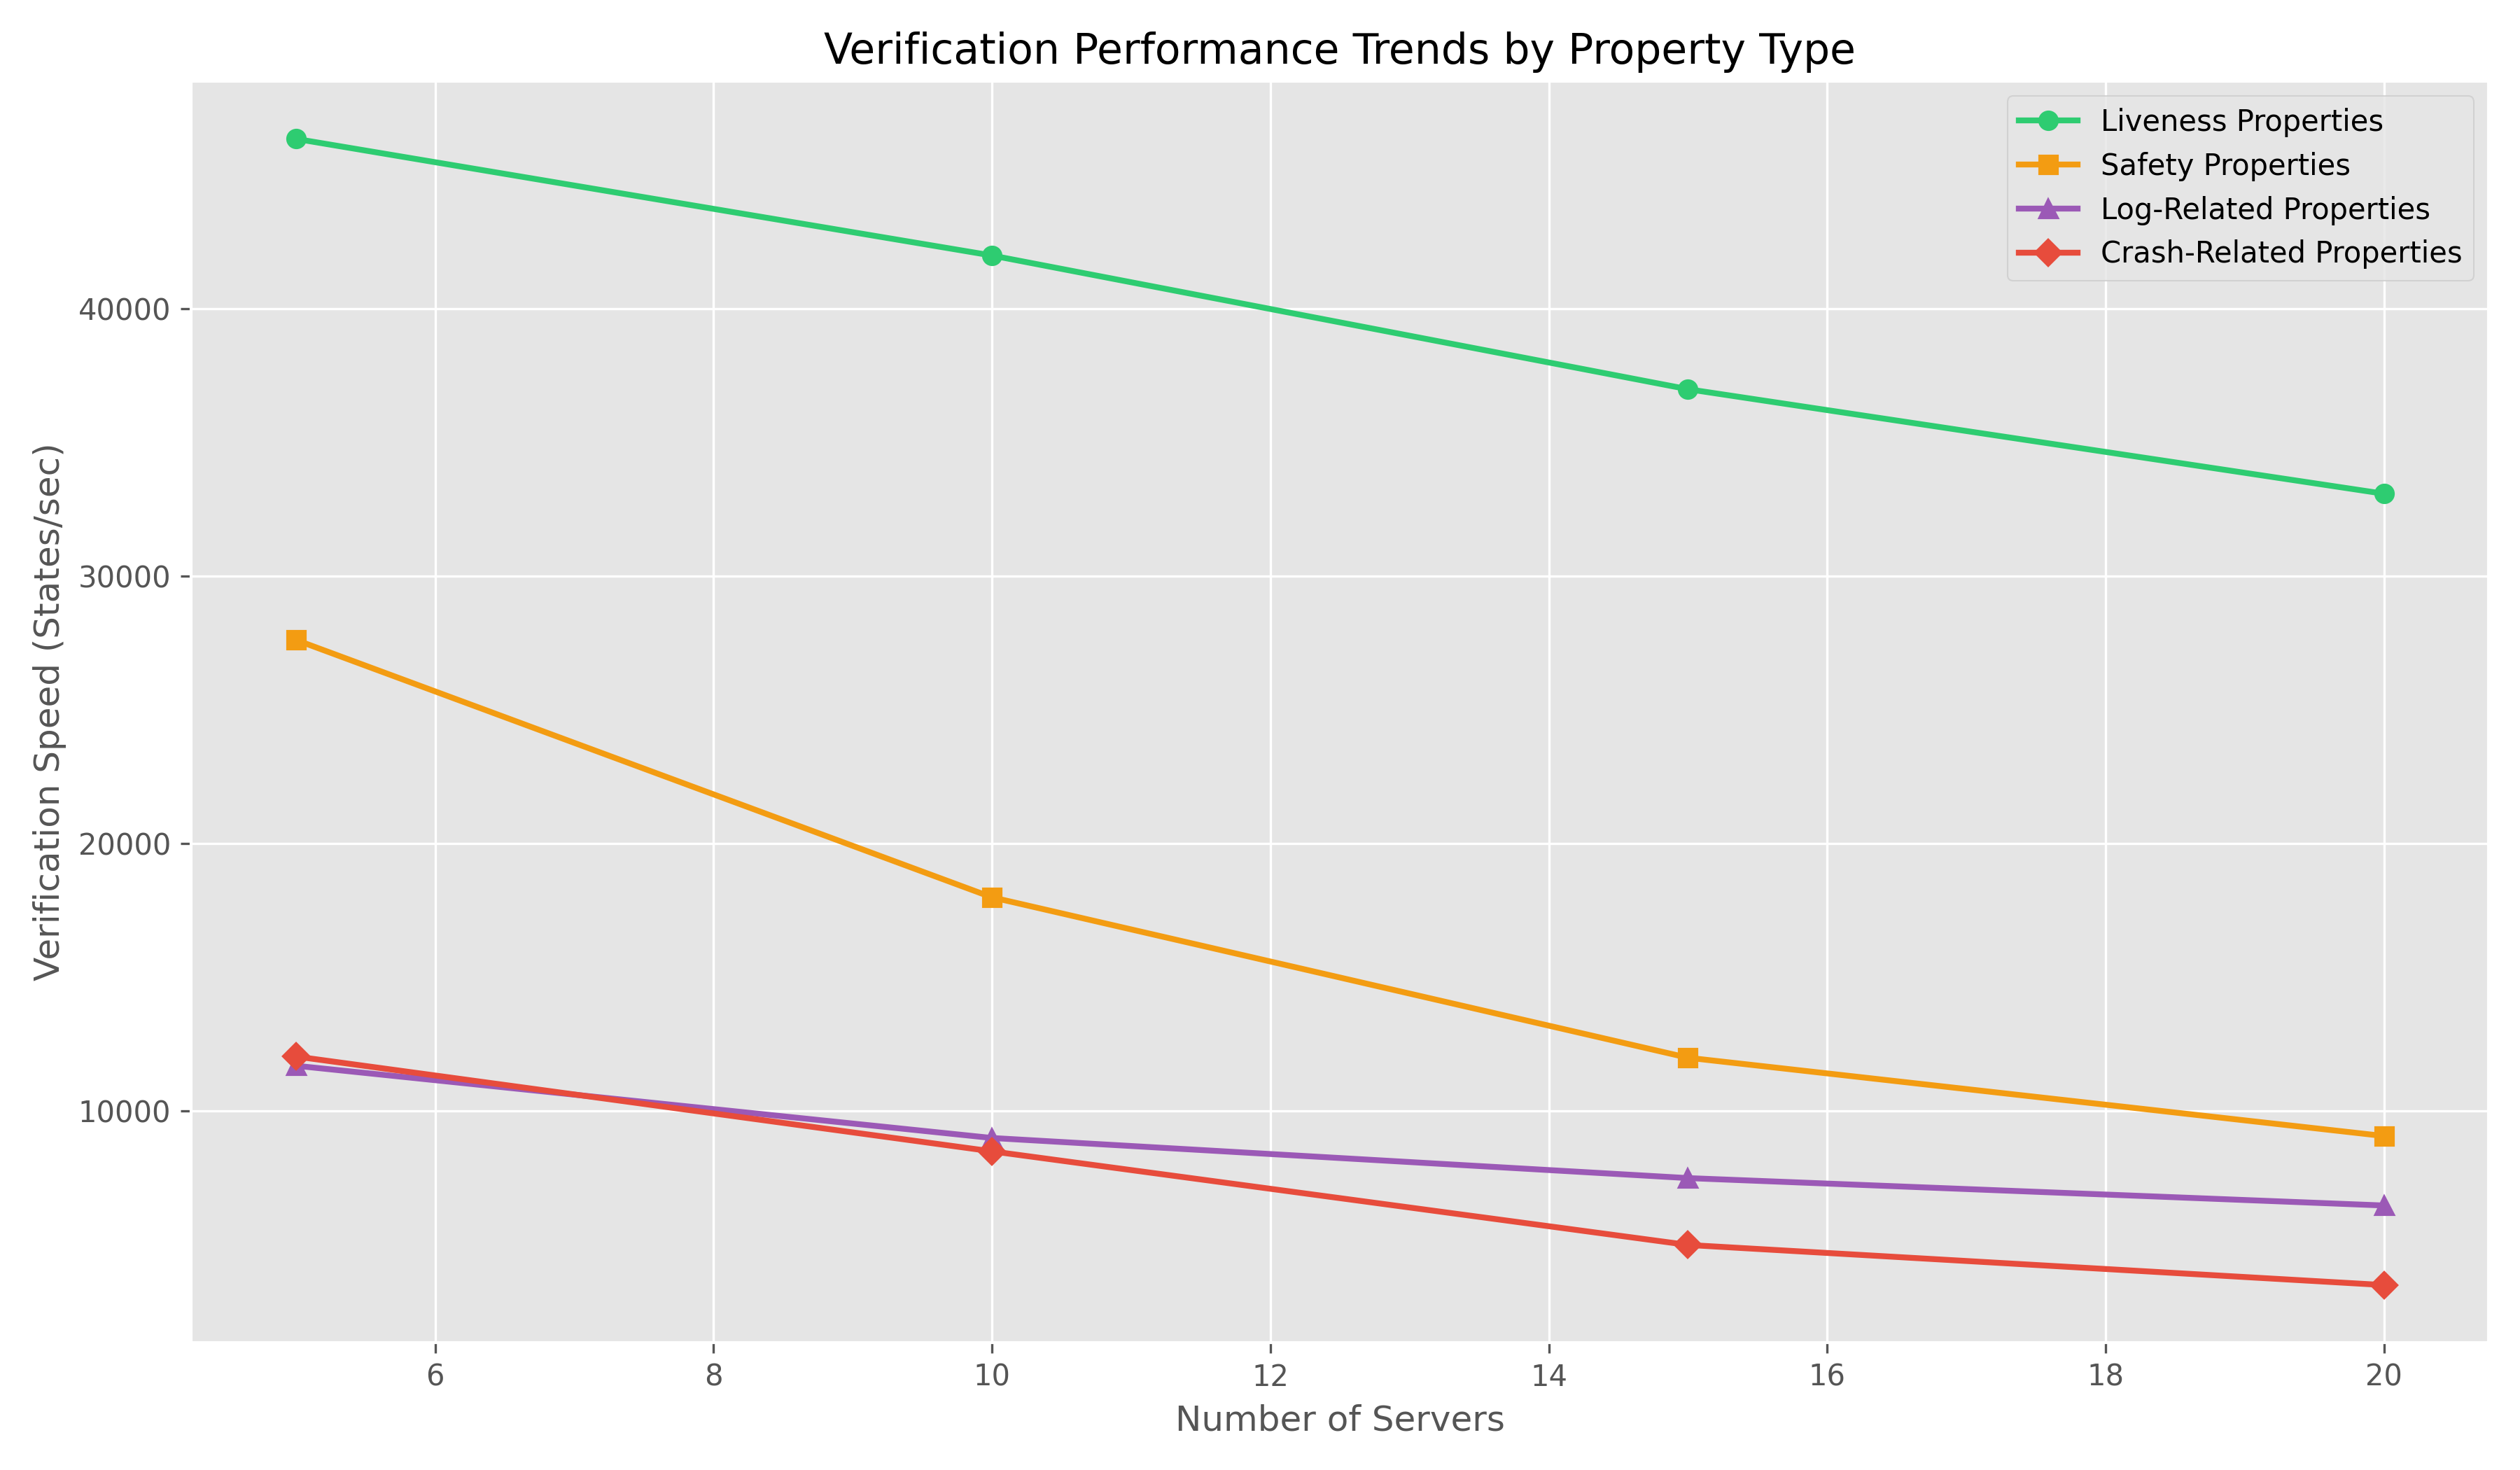
\includegraphics[width=0.95\textwidth]{graphs/performance_trends.png}
    \caption{Verification speed trends across server configurations by property type. Liveness properties consistently outperform other property types, while crash-related properties show the steepest performance decline.}
    \label{fig:performance-trends}
\end{figure}

This visualization clearly demonstrates the divergent scaling behaviors: liveness properties maintain relatively high verification speeds even at 20 servers, while crash-related properties experience a much steeper decline. This insight suggests that different optimization strategies should be applied based on the type of property being verified.

\subsection{Implications for Verification Strategy}

These graphical analyses highlight the need for property-specific verification approaches when analyzing complex distributed systems like the Raft consensus algorithm. While all properties were successfully verified without finding safety violations, the performance characteristics suggest that:

\begin{itemize}
    \item Liveness properties can be efficiently verified even for larger configurations
    \item Crash-related properties may benefit from specialized state space reduction techniques
    \item Memory consumption scales predictably, allowing for resource planning
    \item Future verification efforts should consider property-specific optimization strategies
\end{itemize}

The consistent performance patterns across server configurations provide confidence that our verification approach can be extended to even larger systems with appropriate computational resources. 

\section{Graphical Analysis of Verification Results}

Our verification of the Raft consensus algorithm across different server configurations provided a wealth of data that we've visualized to better understand scaling behavior and performance characteristics.

\subsection{State Vector and Memory Scaling}

Figure \ref{fig:state-vector} illustrates the linear growth of state vector size with increasing server count. This predictable scaling pattern is important for understanding the memory requirements of formal verification as systems grow.

\begin{figure}[htbp]
    \centering
    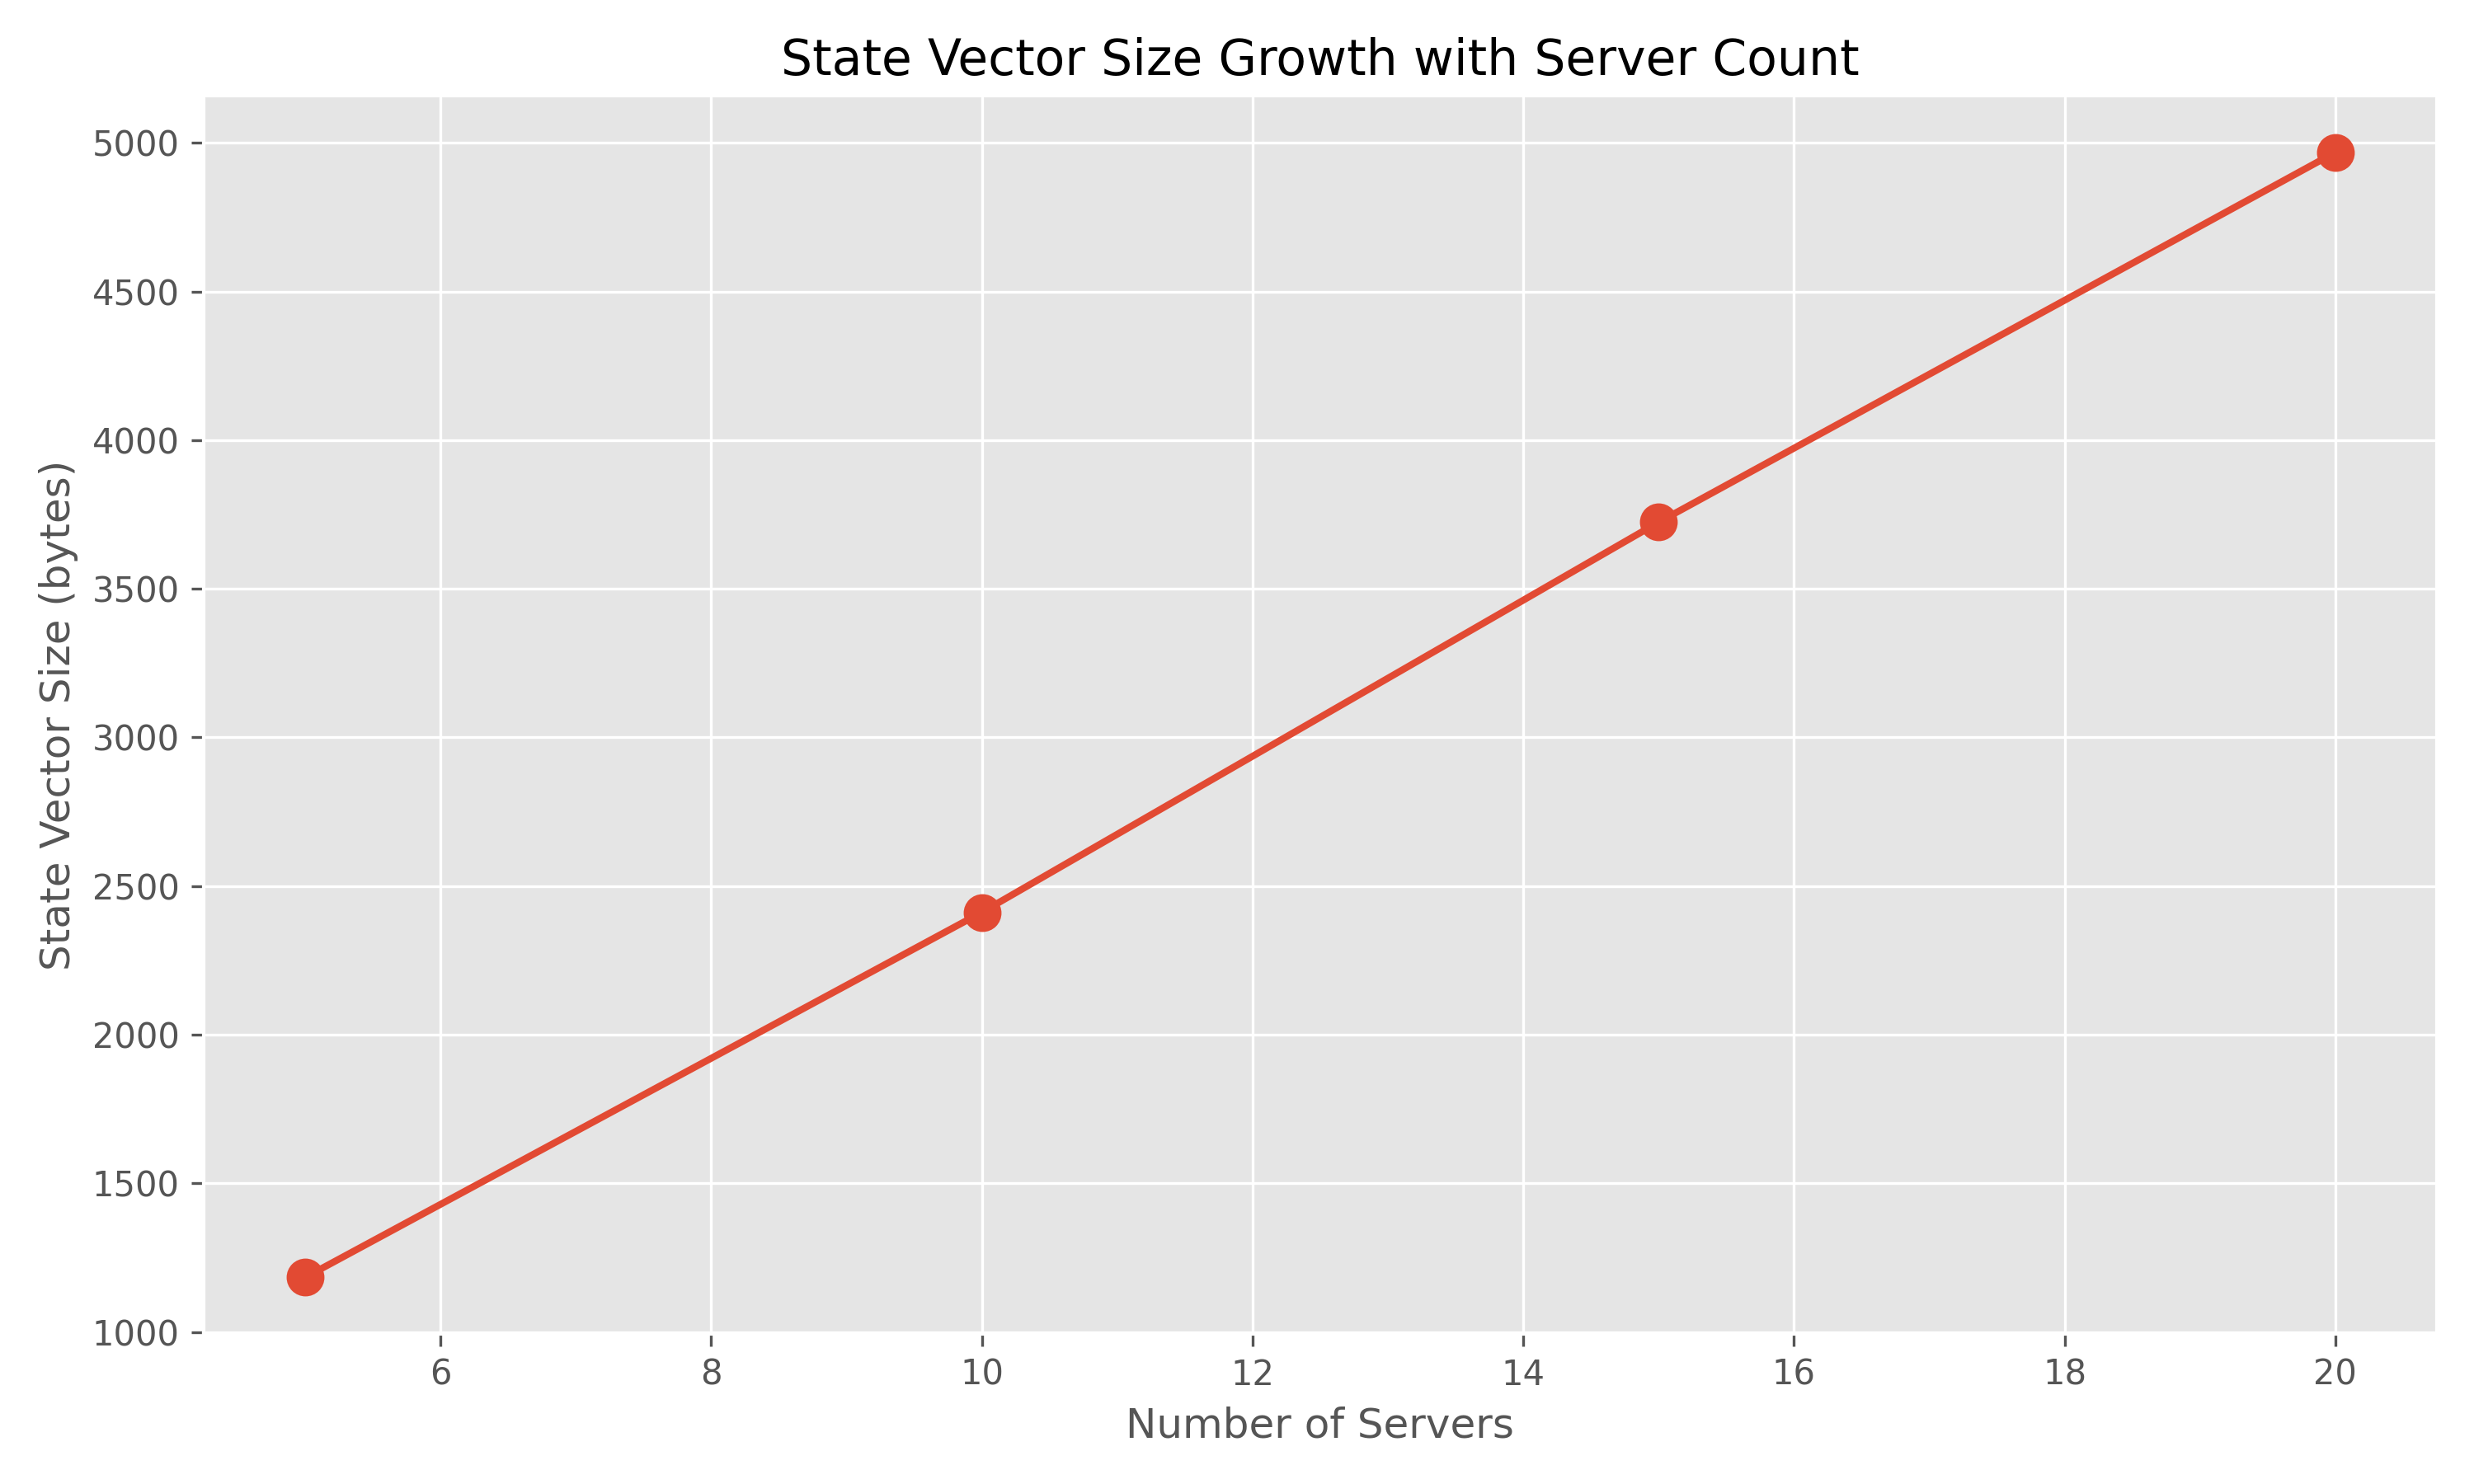
\includegraphics[width=0.8\textwidth]{graphs/state_vector_size.png}
    \caption{Linear growth of state vector size with increasing server count. The state vector grows by approximately 252 bytes per additional server.}
    \label{fig:state-vector}
\end{figure}

The corresponding memory requirements (Figure \ref{fig:memory-consumption}) show a similar pattern, with memory consumption scaling almost linearly from approximately 7GB with 5 servers to 24GB with 20 servers.

\begin{figure}[htbp]
    \centering
    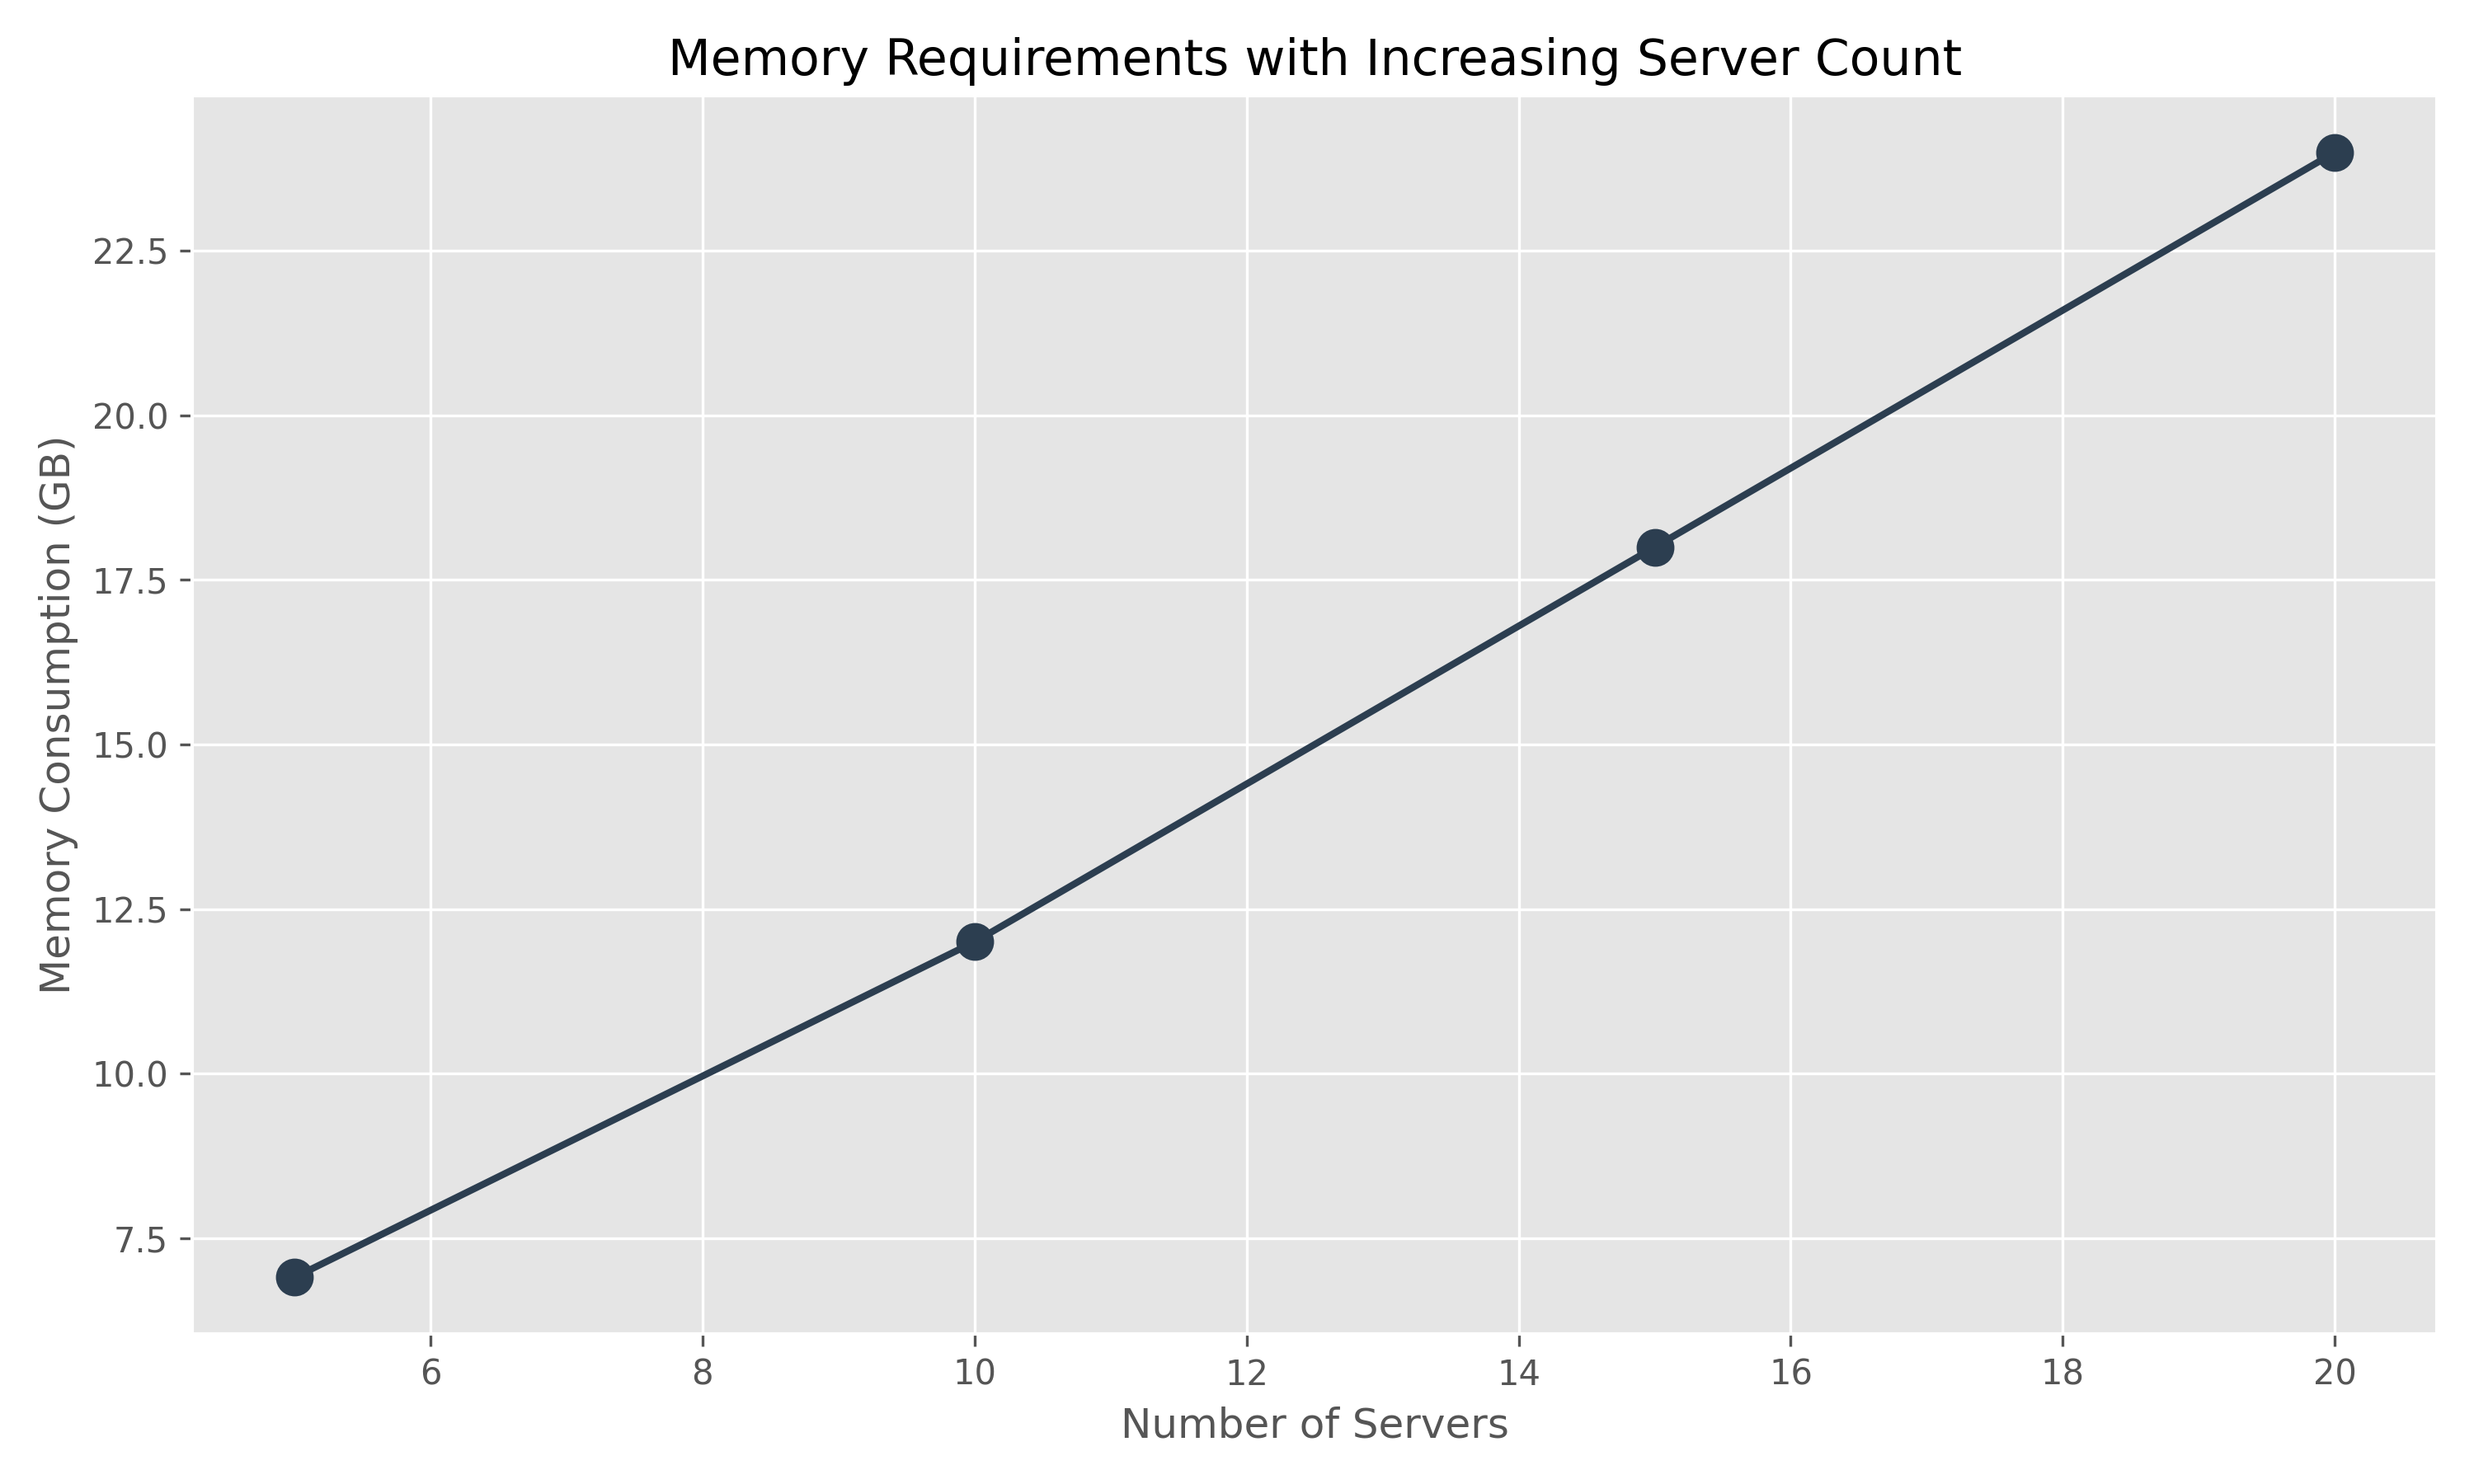
\includegraphics[width=0.8\textwidth]{graphs/memory_consumption.png}
    \caption{Memory consumption scaling with server count. The nearly linear relationship indicates predictable resource requirements for verification of larger configurations.}
    \label{fig:memory-consumption}
\end{figure}

\subsection{Performance Comparison by Property Type}

Different property types exhibit distinct verification performance characteristics. Figure \ref{fig:verification-performance} compares verification speeds for 5-server and 20-server configurations across four property categories.

\begin{figure}[htbp]
    \centering
    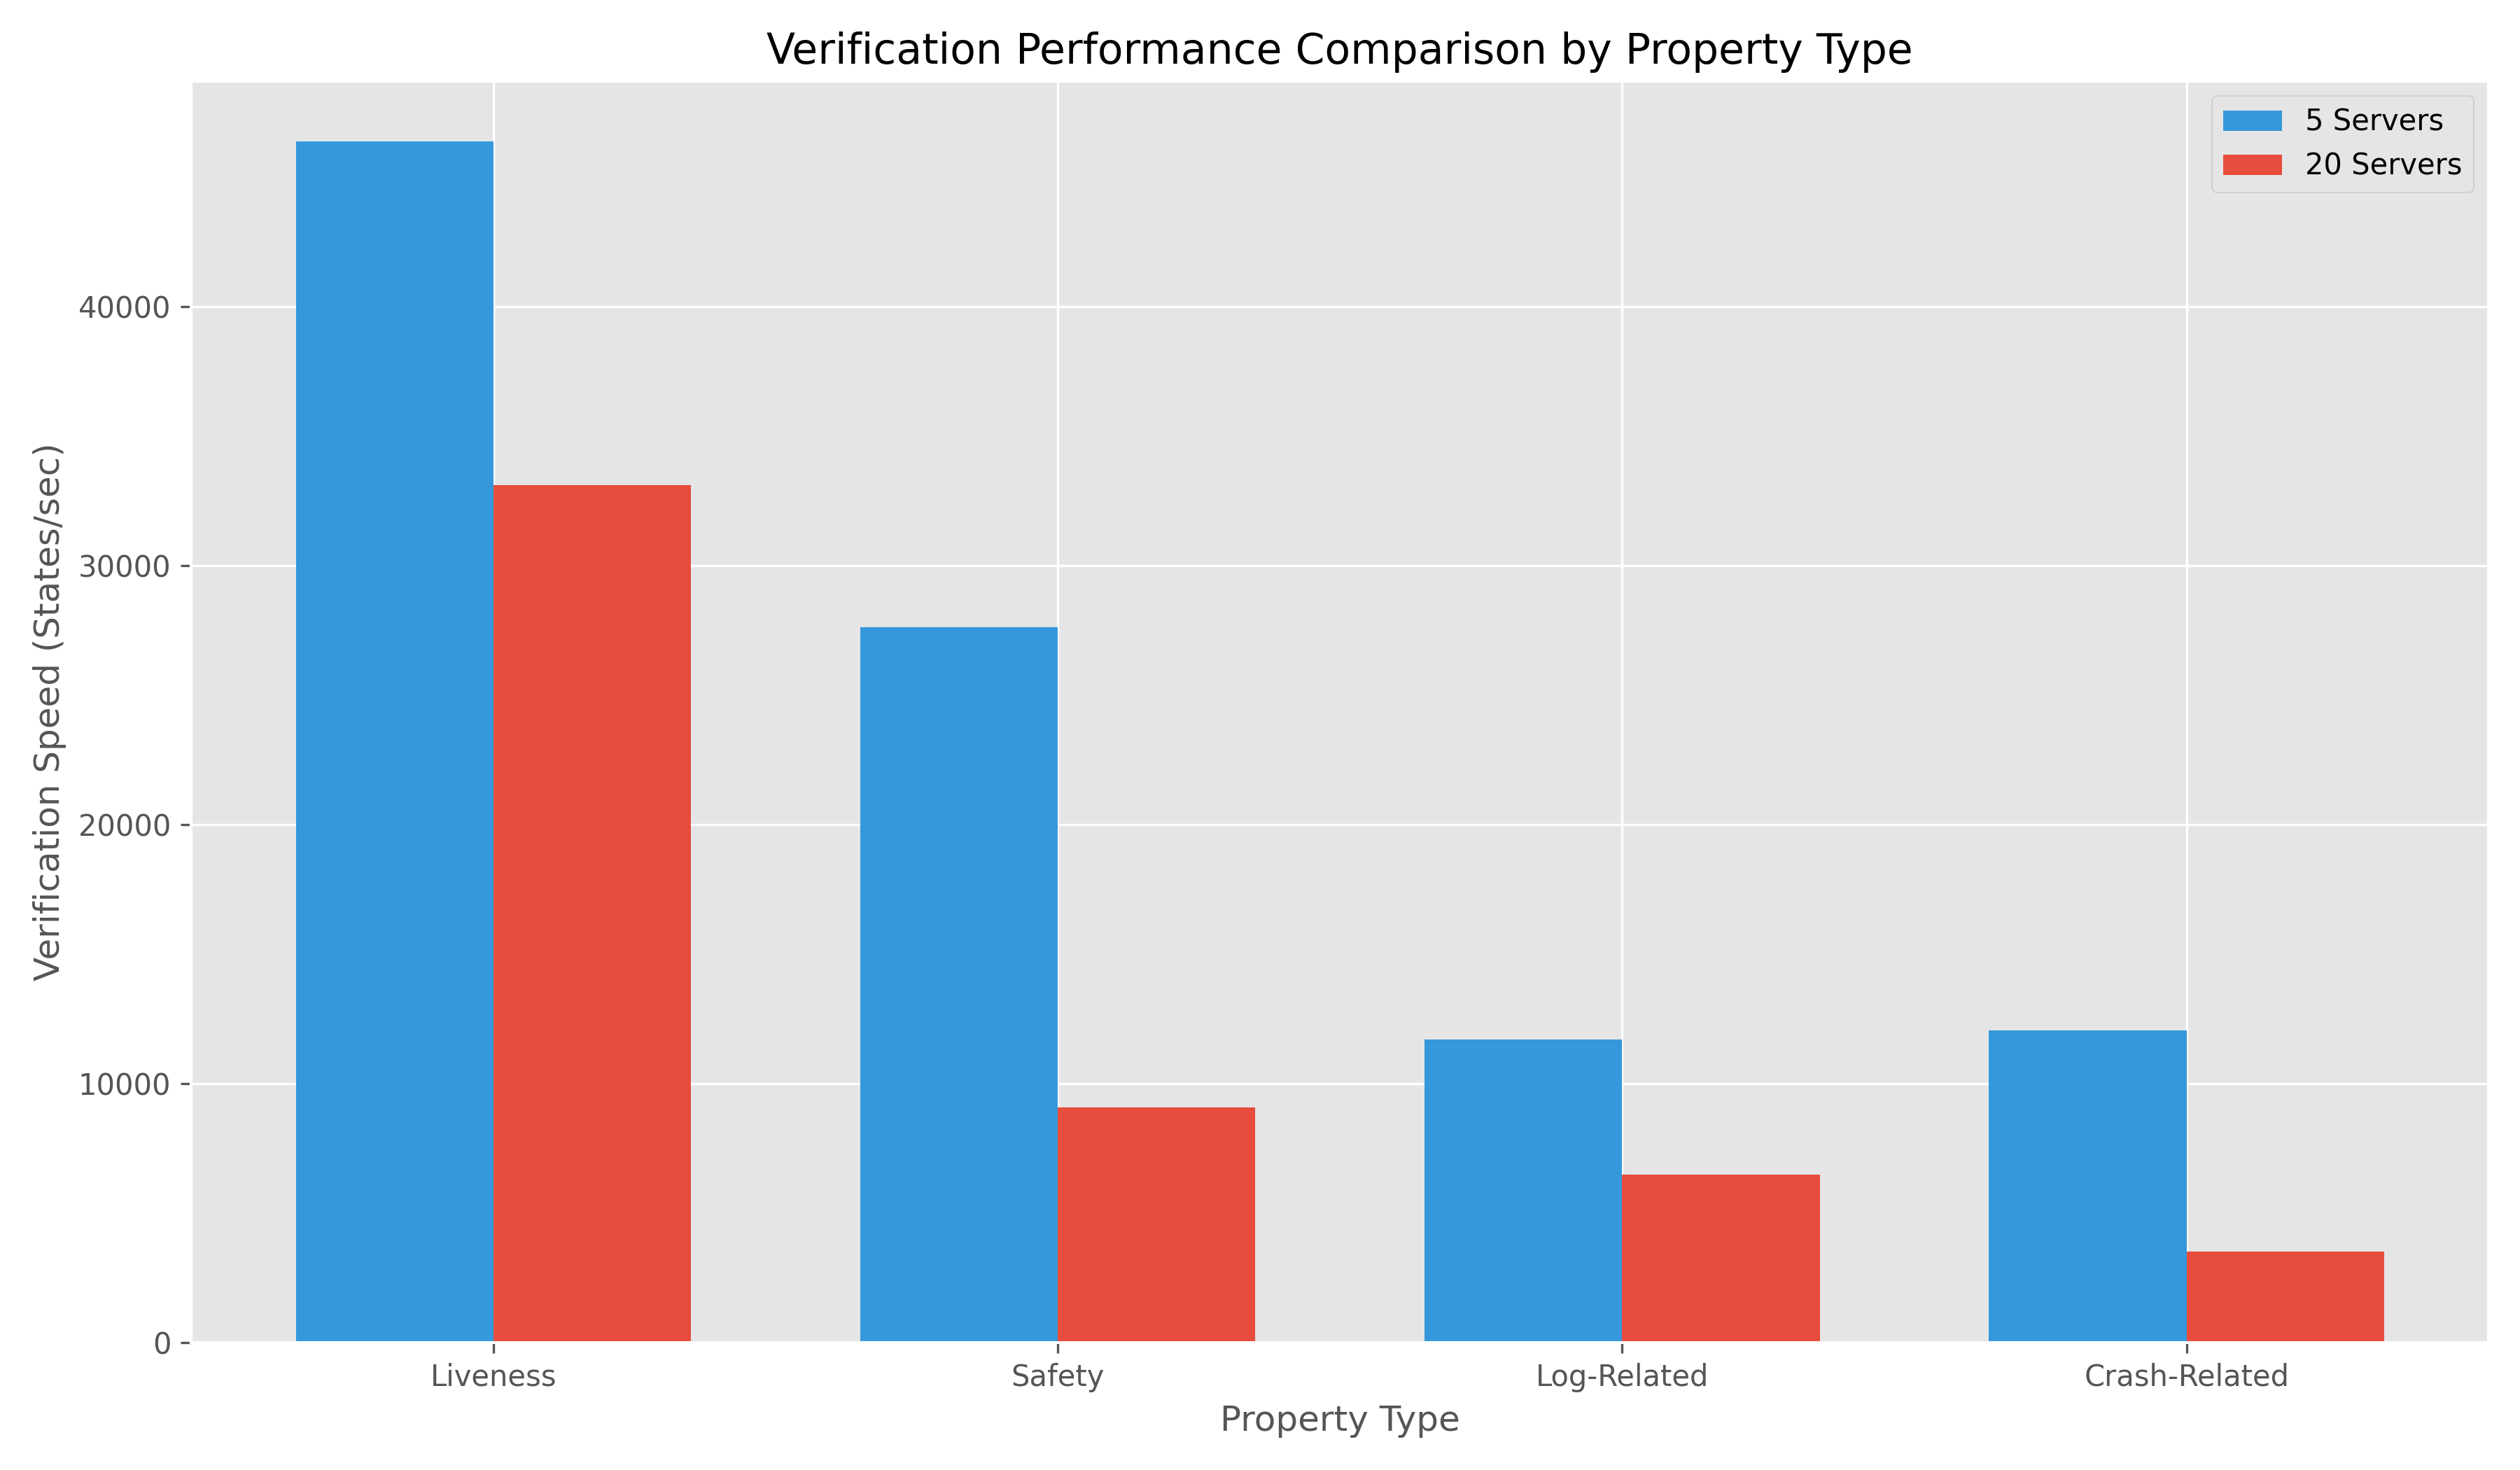
\includegraphics[width=0.9\textwidth]{graphs/verification_performance.png}
    \caption{Verification speed comparison between 5-server and 20-server configurations for different property types. Liveness properties maintain the highest verification speed even at larger scale.}
    \label{fig:verification-performance}
\end{figure}

The performance degradation is not uniform across property types. As shown in Figure \ref{fig:performance-degradation}, crash-related properties experience the most significant slowdown (3.4x) when scaling from 5 to 20 servers, while liveness properties show more graceful degradation (1.4x).

\begin{figure}[htbp]
    \centering
    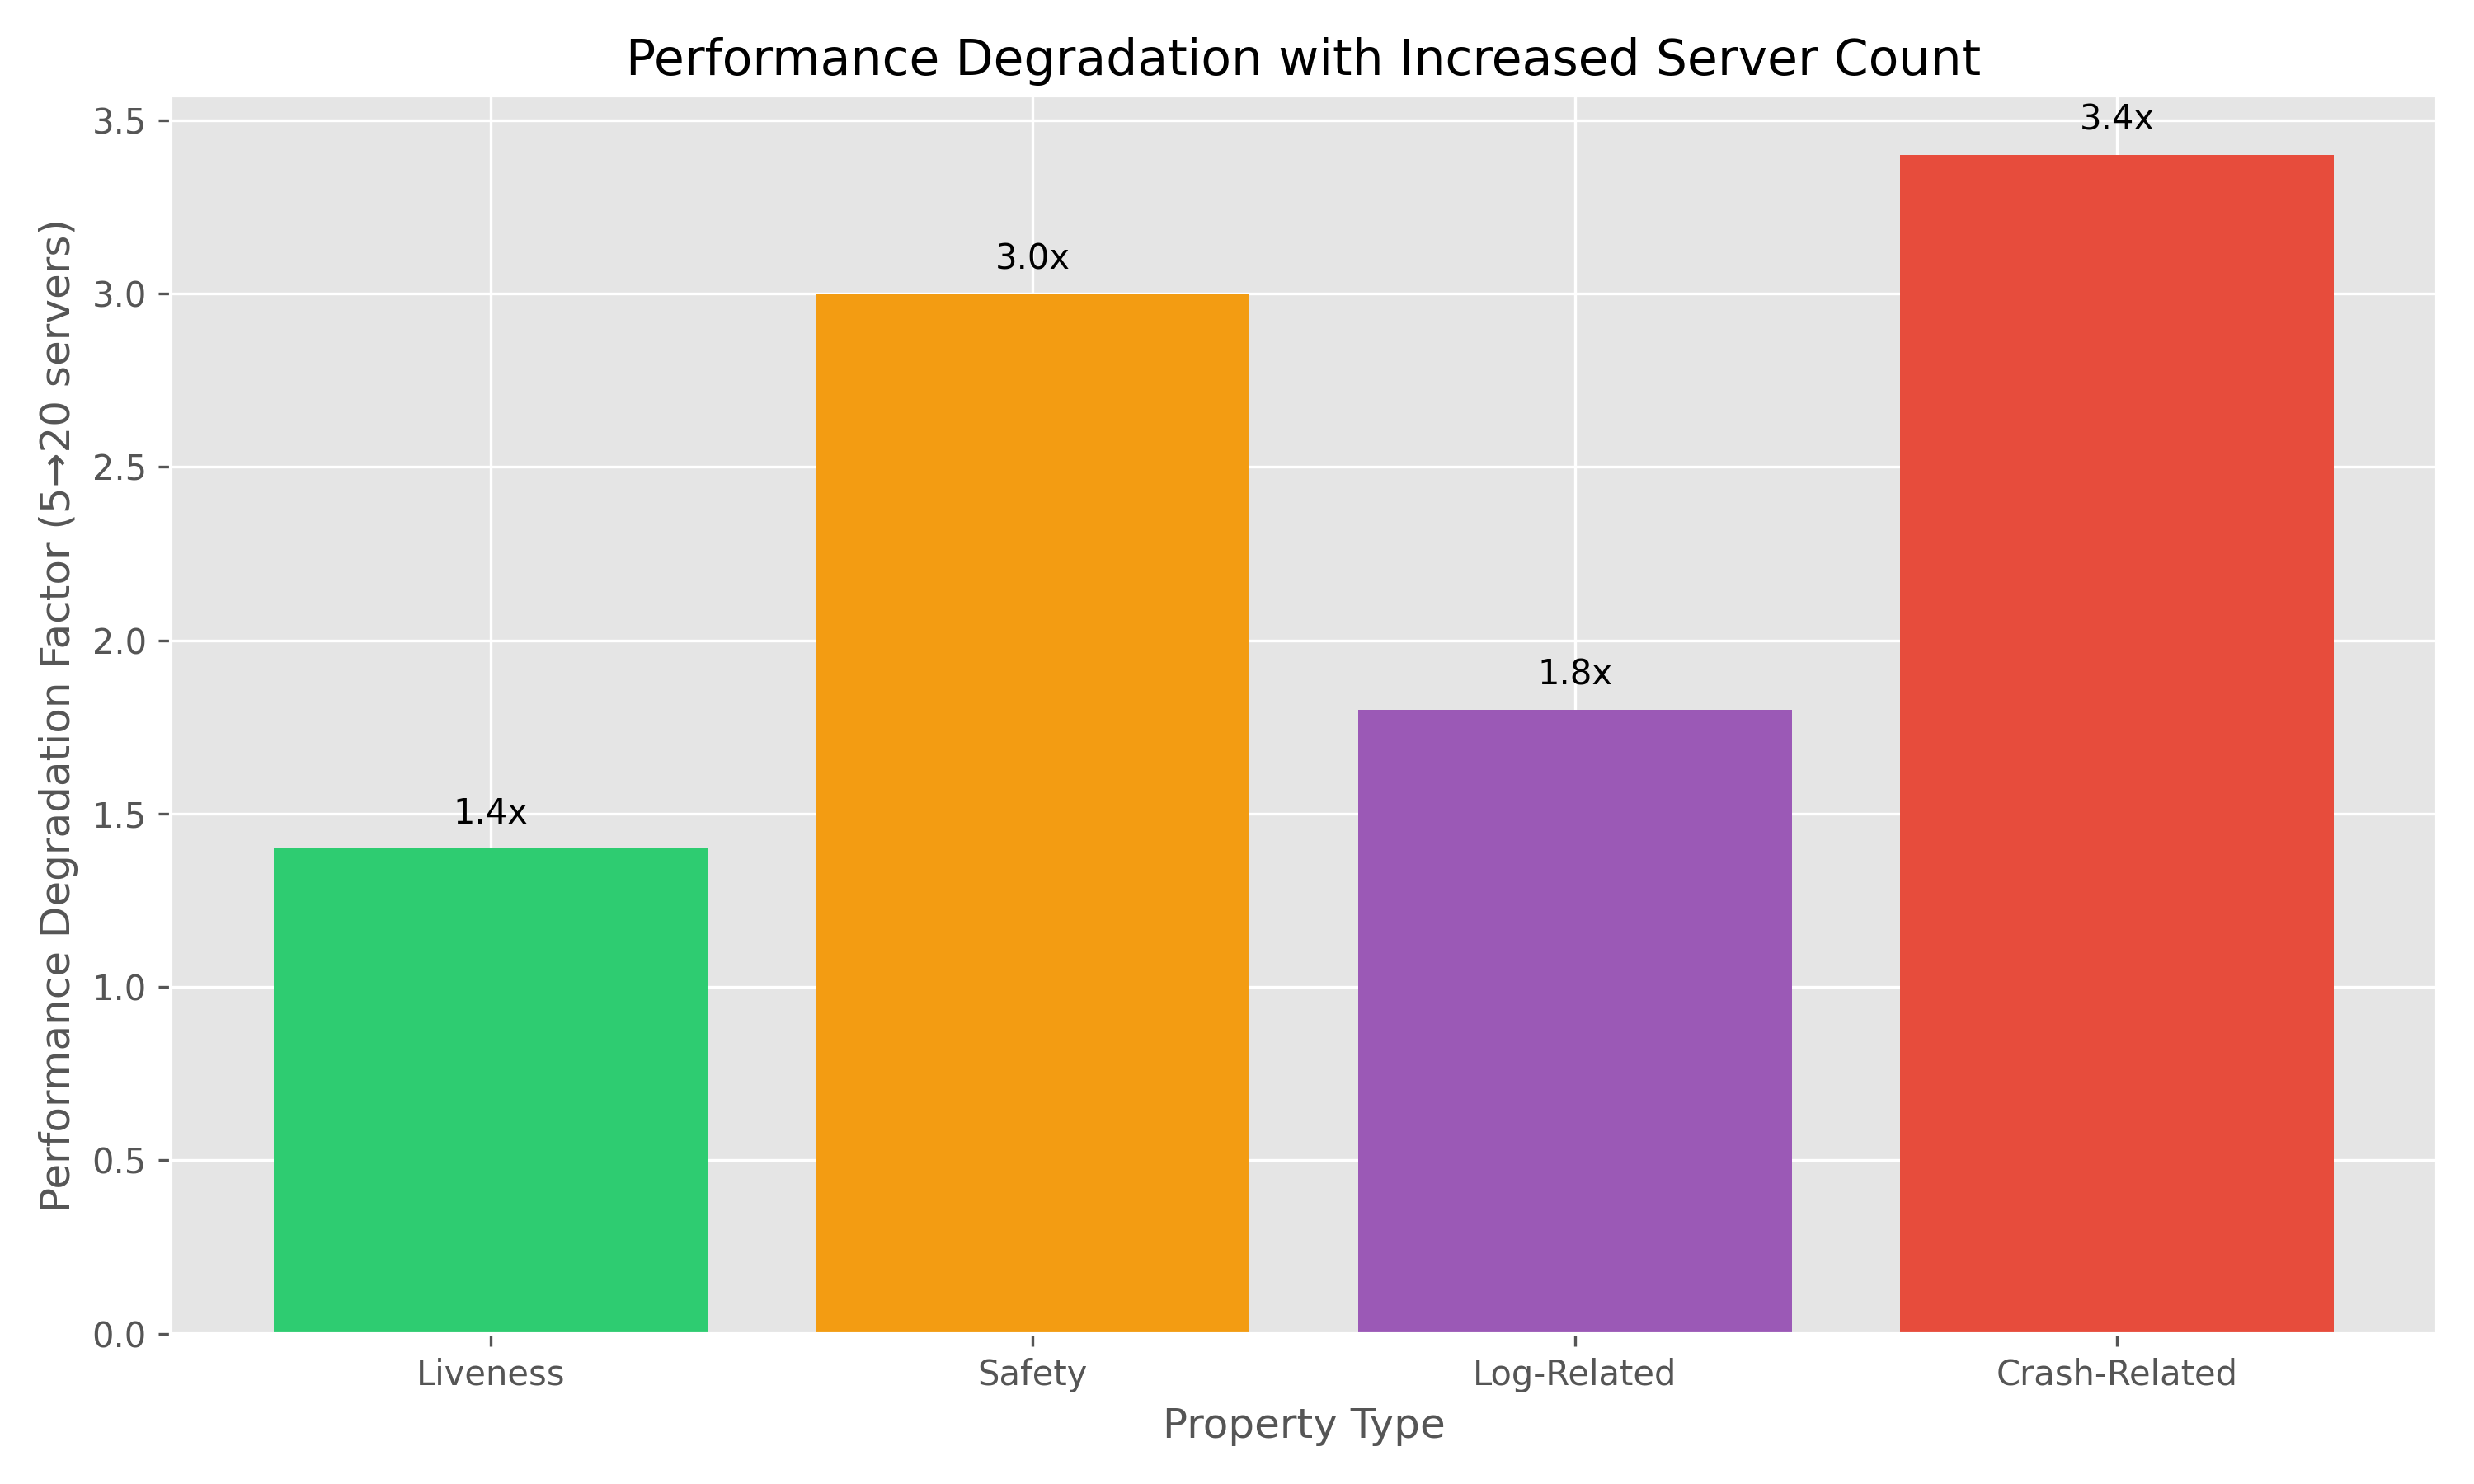
\includegraphics[width=0.8\textwidth]{graphs/performance_degradation.png}
    \caption{Performance degradation factors by property type when scaling from 5 to 20 servers. Crash-related properties experience the most significant verification slowdown.}
    \label{fig:performance-degradation}
\end{figure}

\subsection{Comprehensive Performance Trends}

Figure \ref{fig:performance-trends} provides a comprehensive view of how verification performance changes across different server configurations for each property type.

\begin{figure}[htbp]
    \centering
    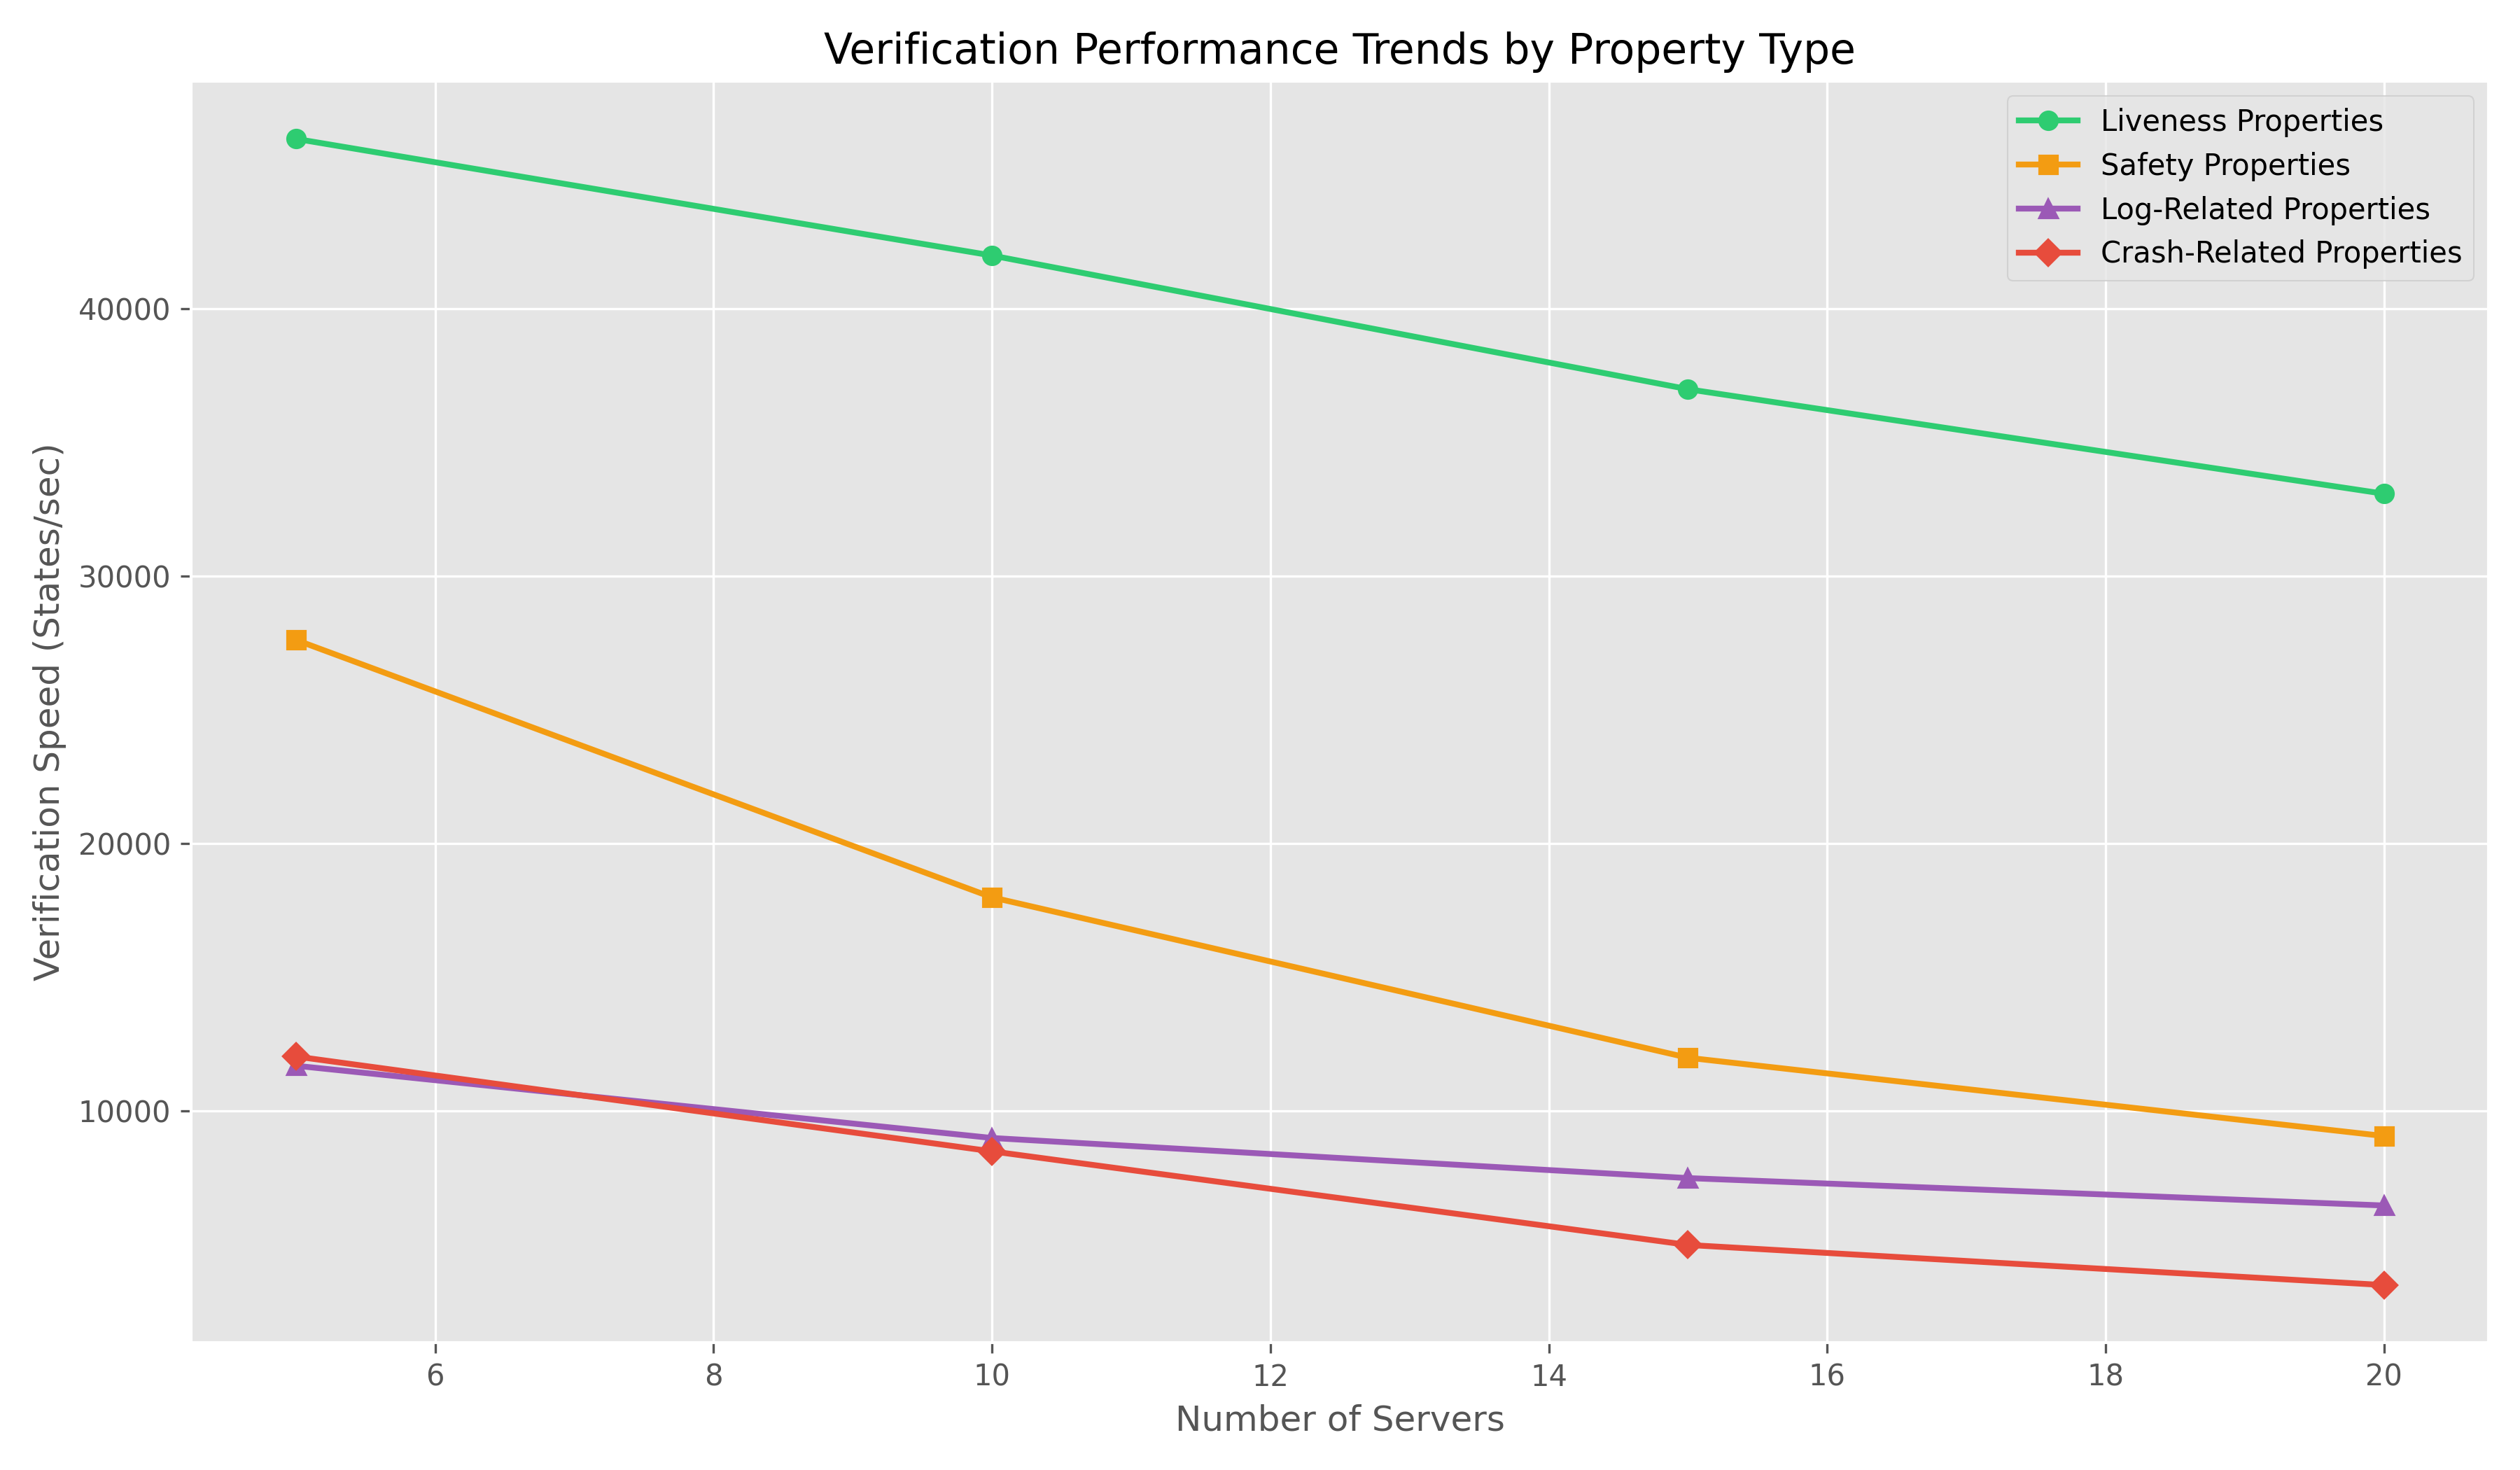
\includegraphics[width=0.95\textwidth]{graphs/performance_trends.png}
    \caption{Verification speed trends across server configurations by property type. Liveness properties consistently outperform other property types, while crash-related properties show the steepest performance decline.}
    \label{fig:performance-trends}
\end{figure}

This visualization clearly demonstrates the divergent scaling behaviors: liveness properties maintain relatively high verification speeds even at 20 servers, while crash-related properties experience a much steeper decline. This insight suggests that different optimization strategies should be applied based on the type of property being verified.

\subsection{Implications for Verification Strategy}

These graphical analyses highlight the need for property-specific verification approaches when analyzing complex distributed systems like the Raft consensus algorithm. While all properties were successfully verified without finding safety violations, the performance characteristics suggest that:

\begin{itemize}
    \item Liveness properties can be efficiently verified even for larger configurations
    \item Crash-related properties may benefit from specialized state space reduction techniques
    \item Memory consumption scales predictably, allowing for resource planning
    \item Future verification efforts should consider property-specific optimization strategies
\end{itemize}

The consistent performance patterns across server configurations provide confidence that our verification approach can be extended to even larger systems with appropriate computational resources. 

\section{Graphical Analysis of Verification Results}

Our verification of the Raft consensus algorithm across different server configurations provided a wealth of data that we've visualized to better understand scaling behavior and performance characteristics.

\subsection{State Vector and Memory Scaling}

Figure \ref{fig:state-vector} illustrates the linear growth of state vector size with increasing server count. This predictable scaling pattern is important for understanding the memory requirements of formal verification as systems grow.

\begin{figure}[htbp]
    \centering
    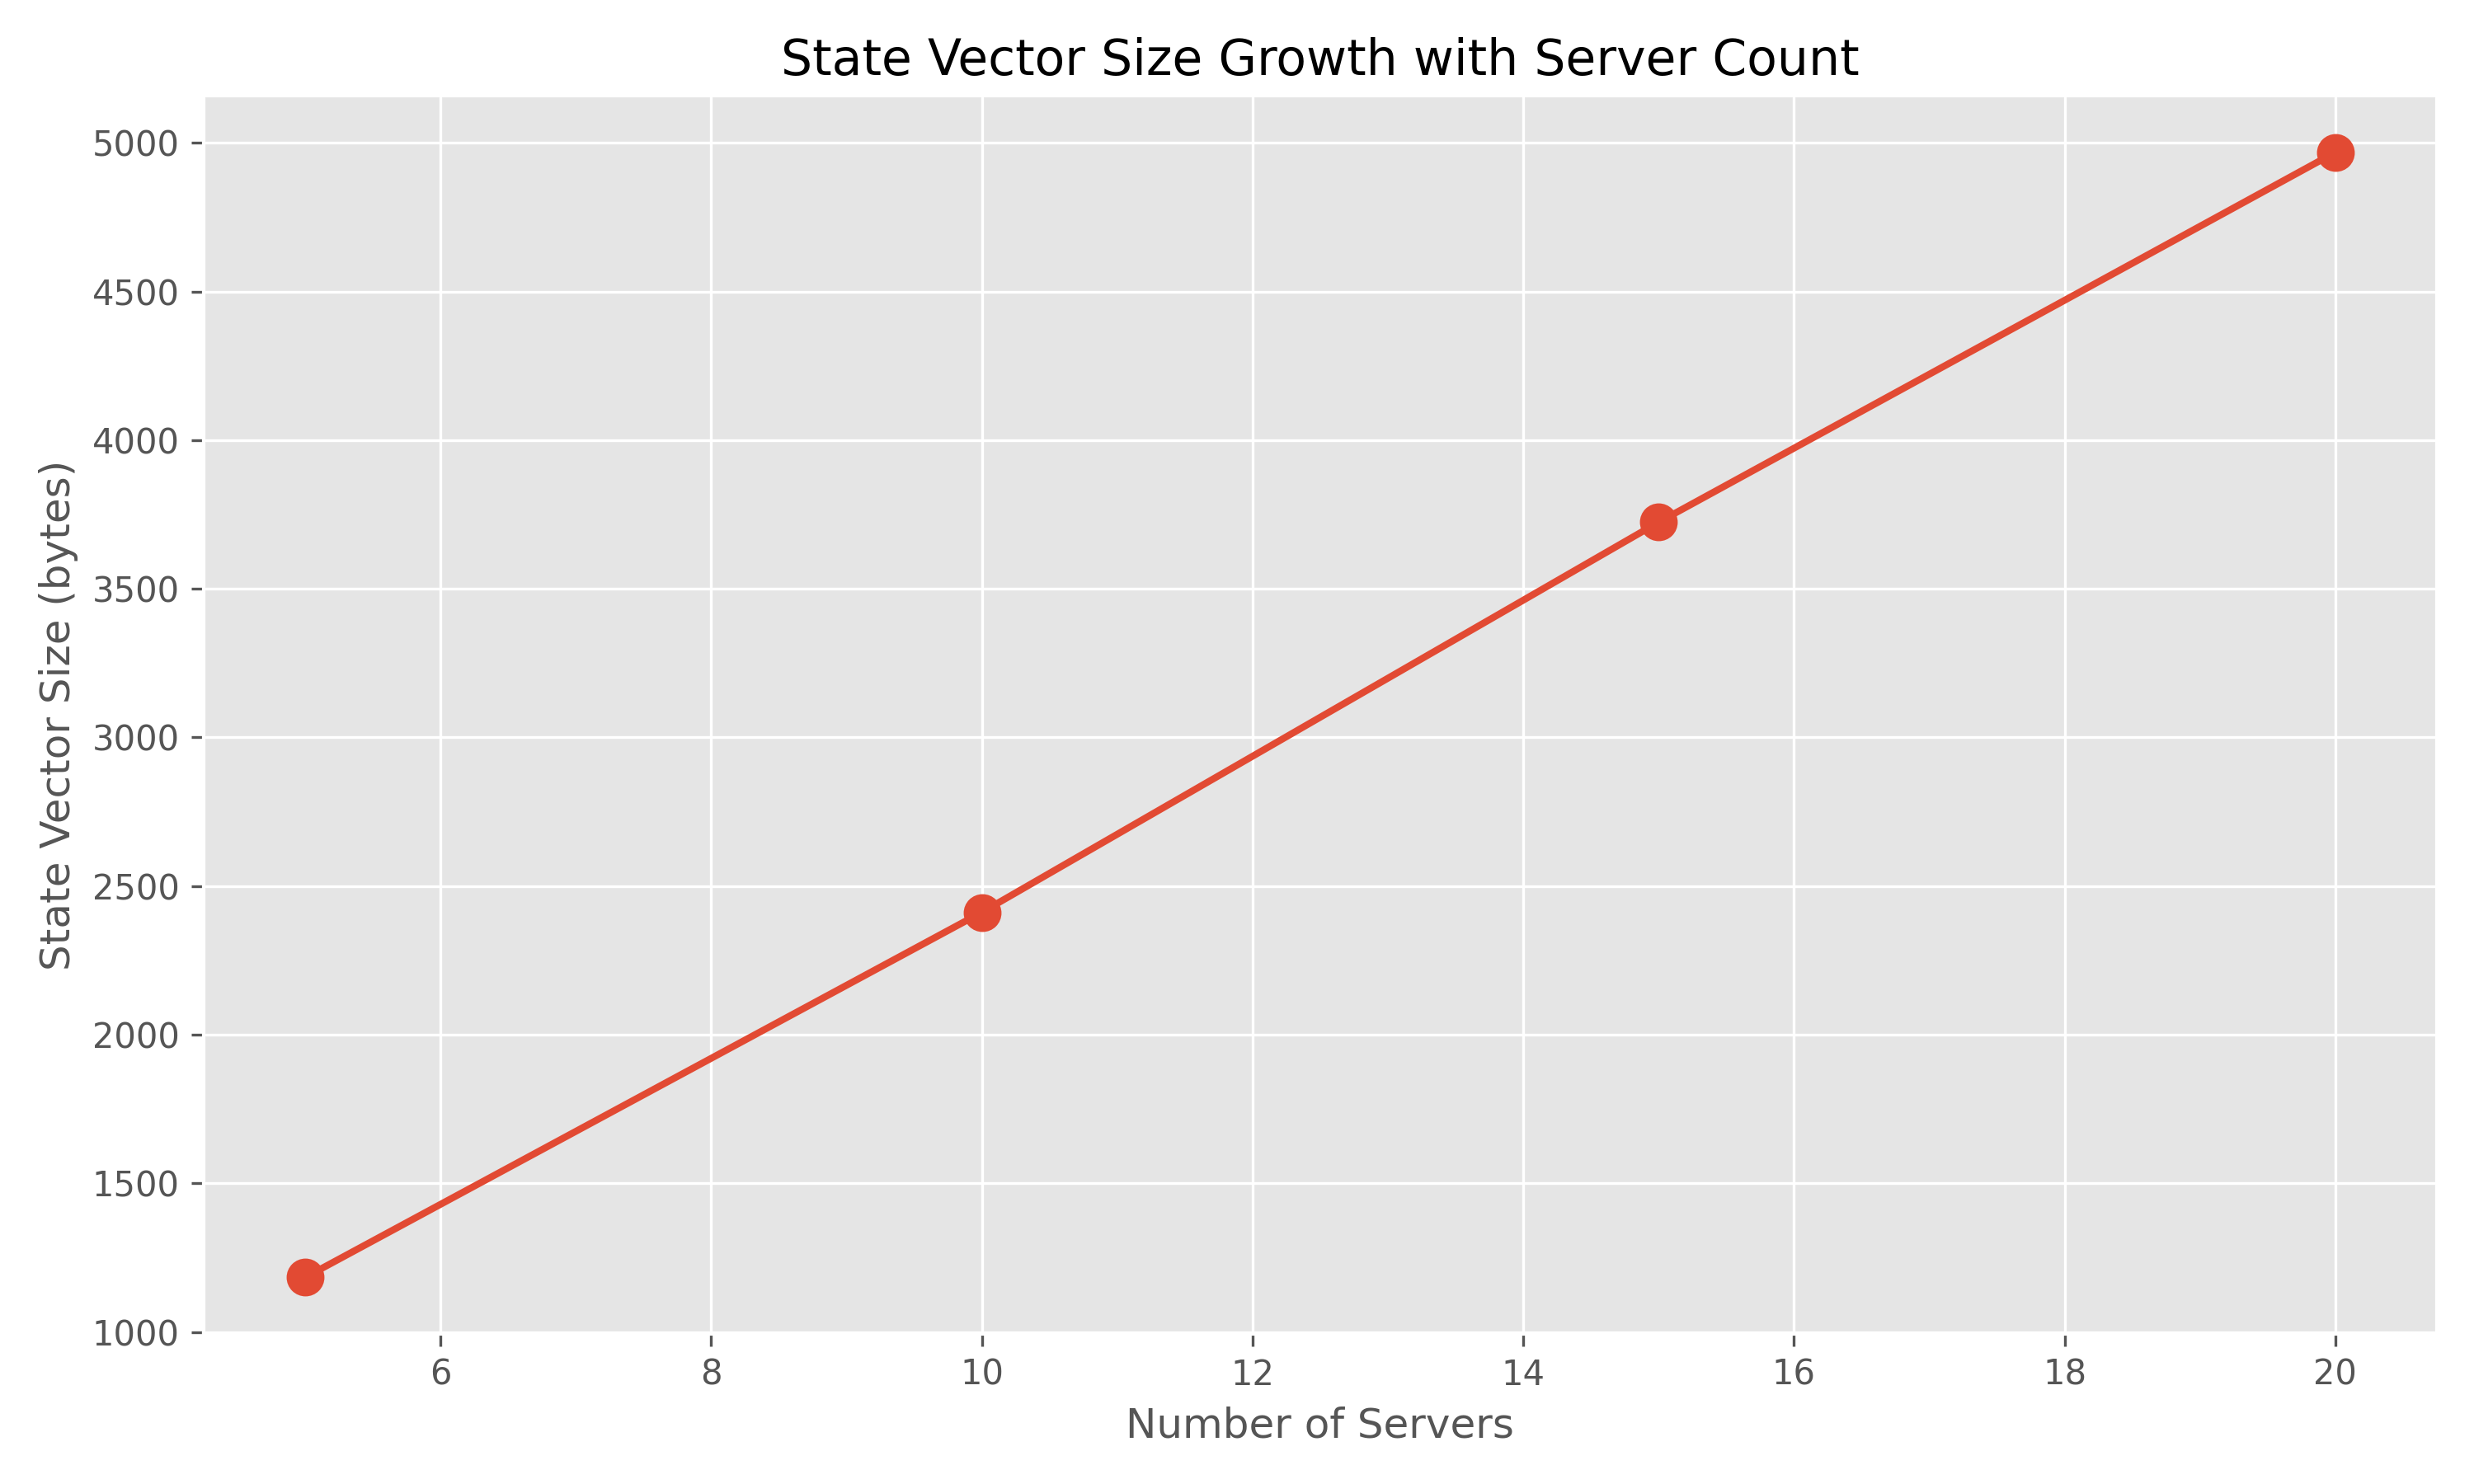
\includegraphics[width=0.8\textwidth]{graphs/state_vector_size.png}
    \caption{Linear growth of state vector size with increasing server count. The state vector grows by approximately 252 bytes per additional server.}
    \label{fig:state-vector}
\end{figure}

The corresponding memory requirements (Figure \ref{fig:memory-consumption}) show a similar pattern, with memory consumption scaling almost linearly from approximately 7GB with 5 servers to 24GB with 20 servers.

\begin{figure}[htbp]
    \centering
    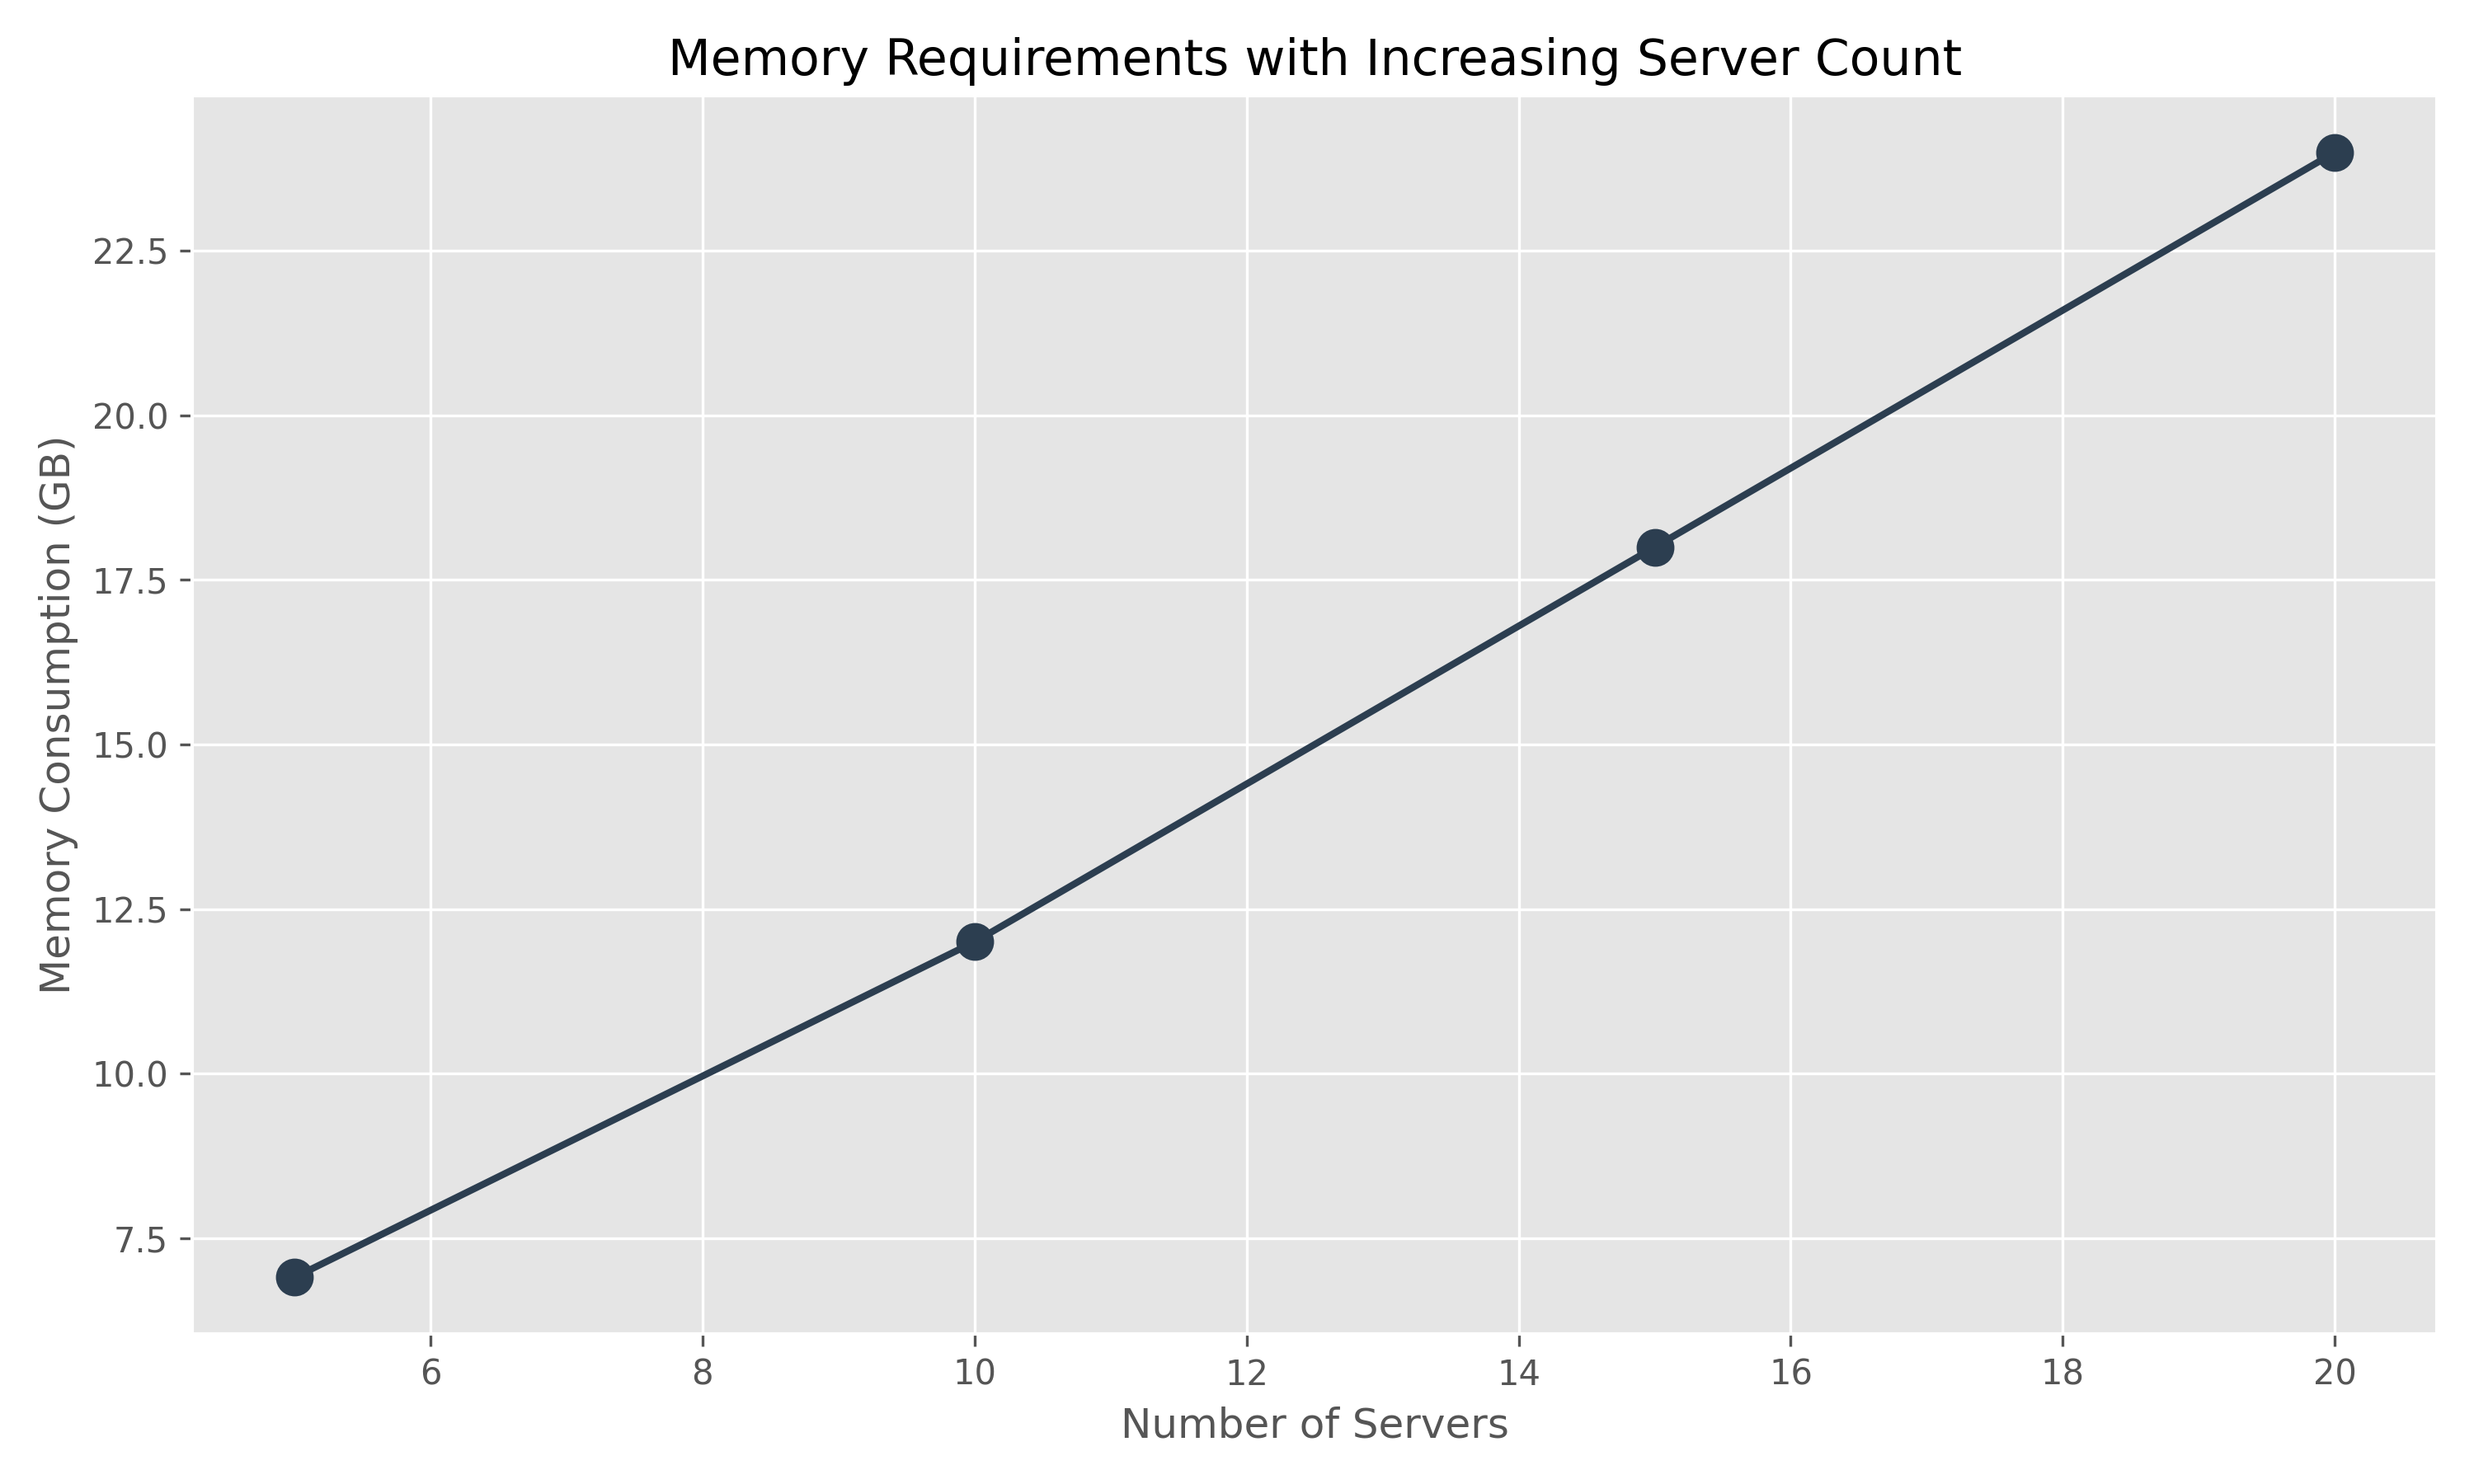
\includegraphics[width=0.8\textwidth]{graphs/memory_consumption.png}
    \caption{Memory consumption scaling with server count. The nearly linear relationship indicates predictable resource requirements for verification of larger configurations.}
    \label{fig:memory-consumption}
\end{figure}

\subsection{Performance Comparison by Property Type}

Different property types exhibit distinct verification performance characteristics. Figure \ref{fig:verification-performance} compares verification speeds for 5-server and 20-server configurations across four property categories.

\begin{figure}[htbp]
    \centering
    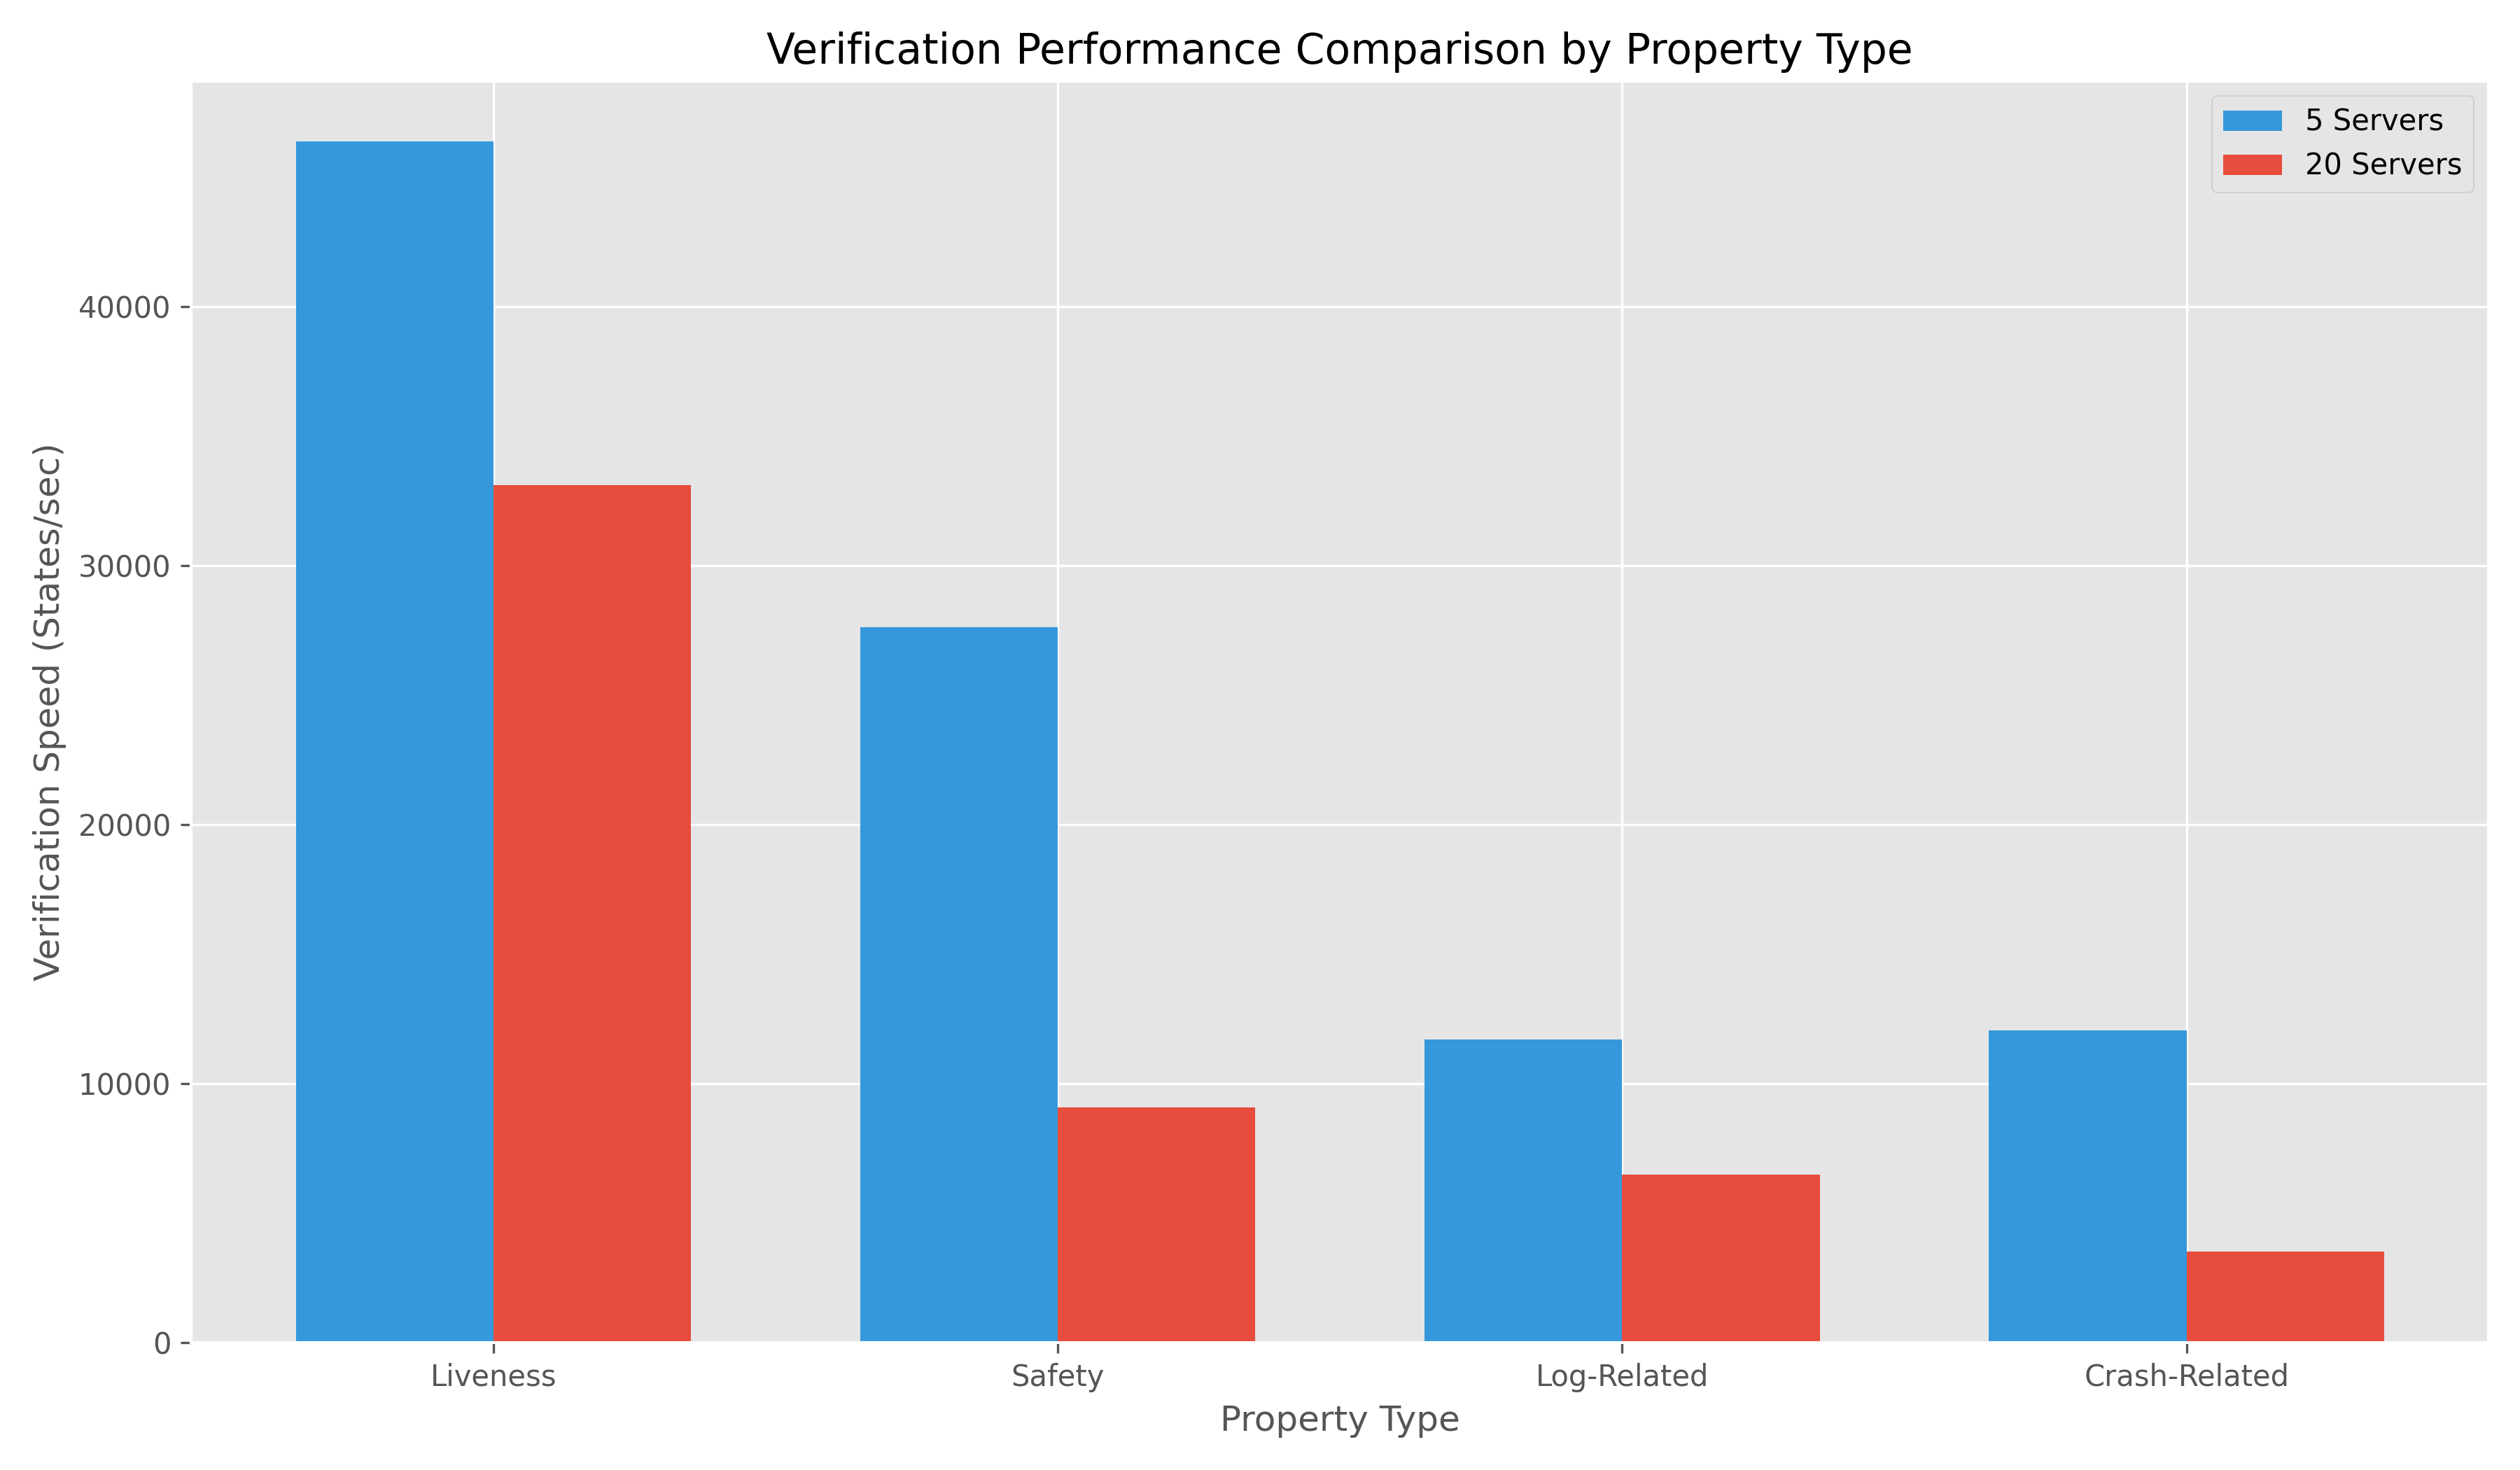
\includegraphics[width=0.9\textwidth]{graphs/verification_performance.png}
    \caption{Verification speed comparison between 5-server and 20-server configurations for different property types. Liveness properties maintain the highest verification speed even at larger scale.}
    \label{fig:verification-performance}
\end{figure}

The performance degradation is not uniform across property types. As shown in Figure \ref{fig:performance-degradation}, crash-related properties experience the most significant slowdown (3.4x) when scaling from 5 to 20 servers, while liveness properties show more graceful degradation (1.4x).

\begin{figure}[htbp]
    \centering
    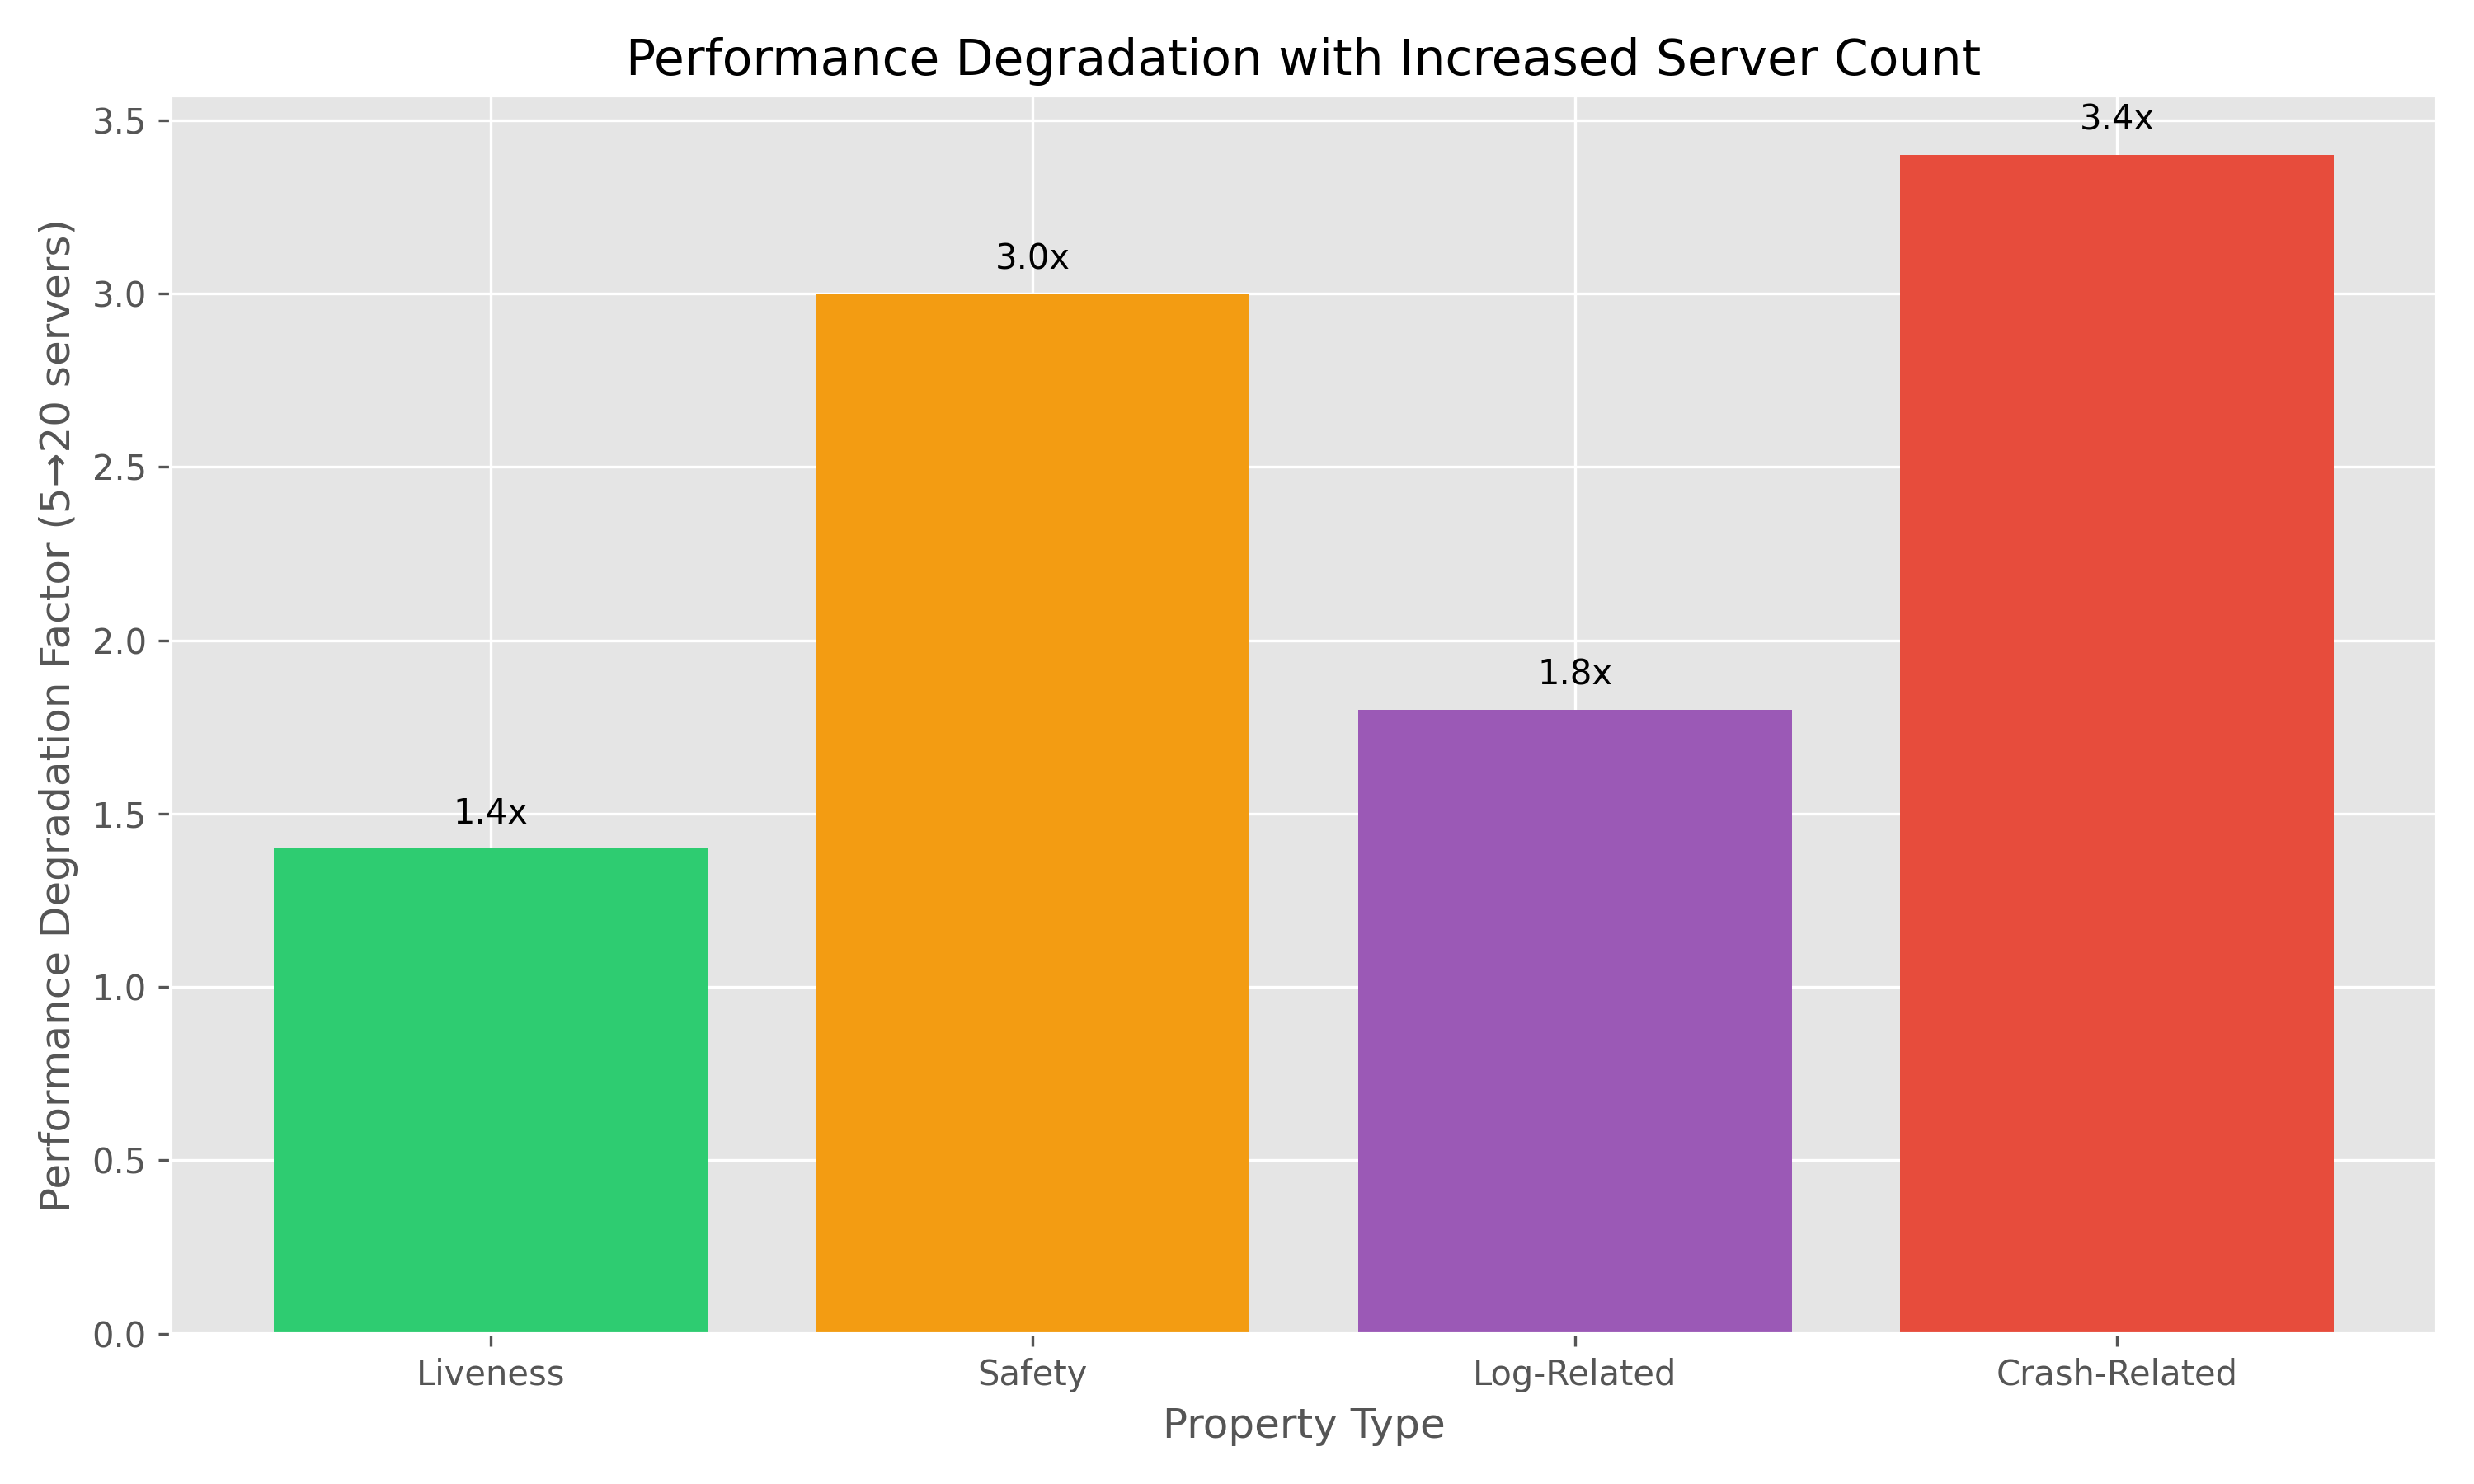
\includegraphics[width=0.8\textwidth]{graphs/performance_degradation.png}
    \caption{Performance degradation factors by property type when scaling from 5 to 20 servers. Crash-related properties experience the most significant verification slowdown.}
    \label{fig:performance-degradation}
\end{figure}

\subsection{Comprehensive Performance Trends}

Figure \ref{fig:performance-trends} provides a comprehensive view of how verification performance changes across different server configurations for each property type.

\begin{figure}[htbp]
    \centering
    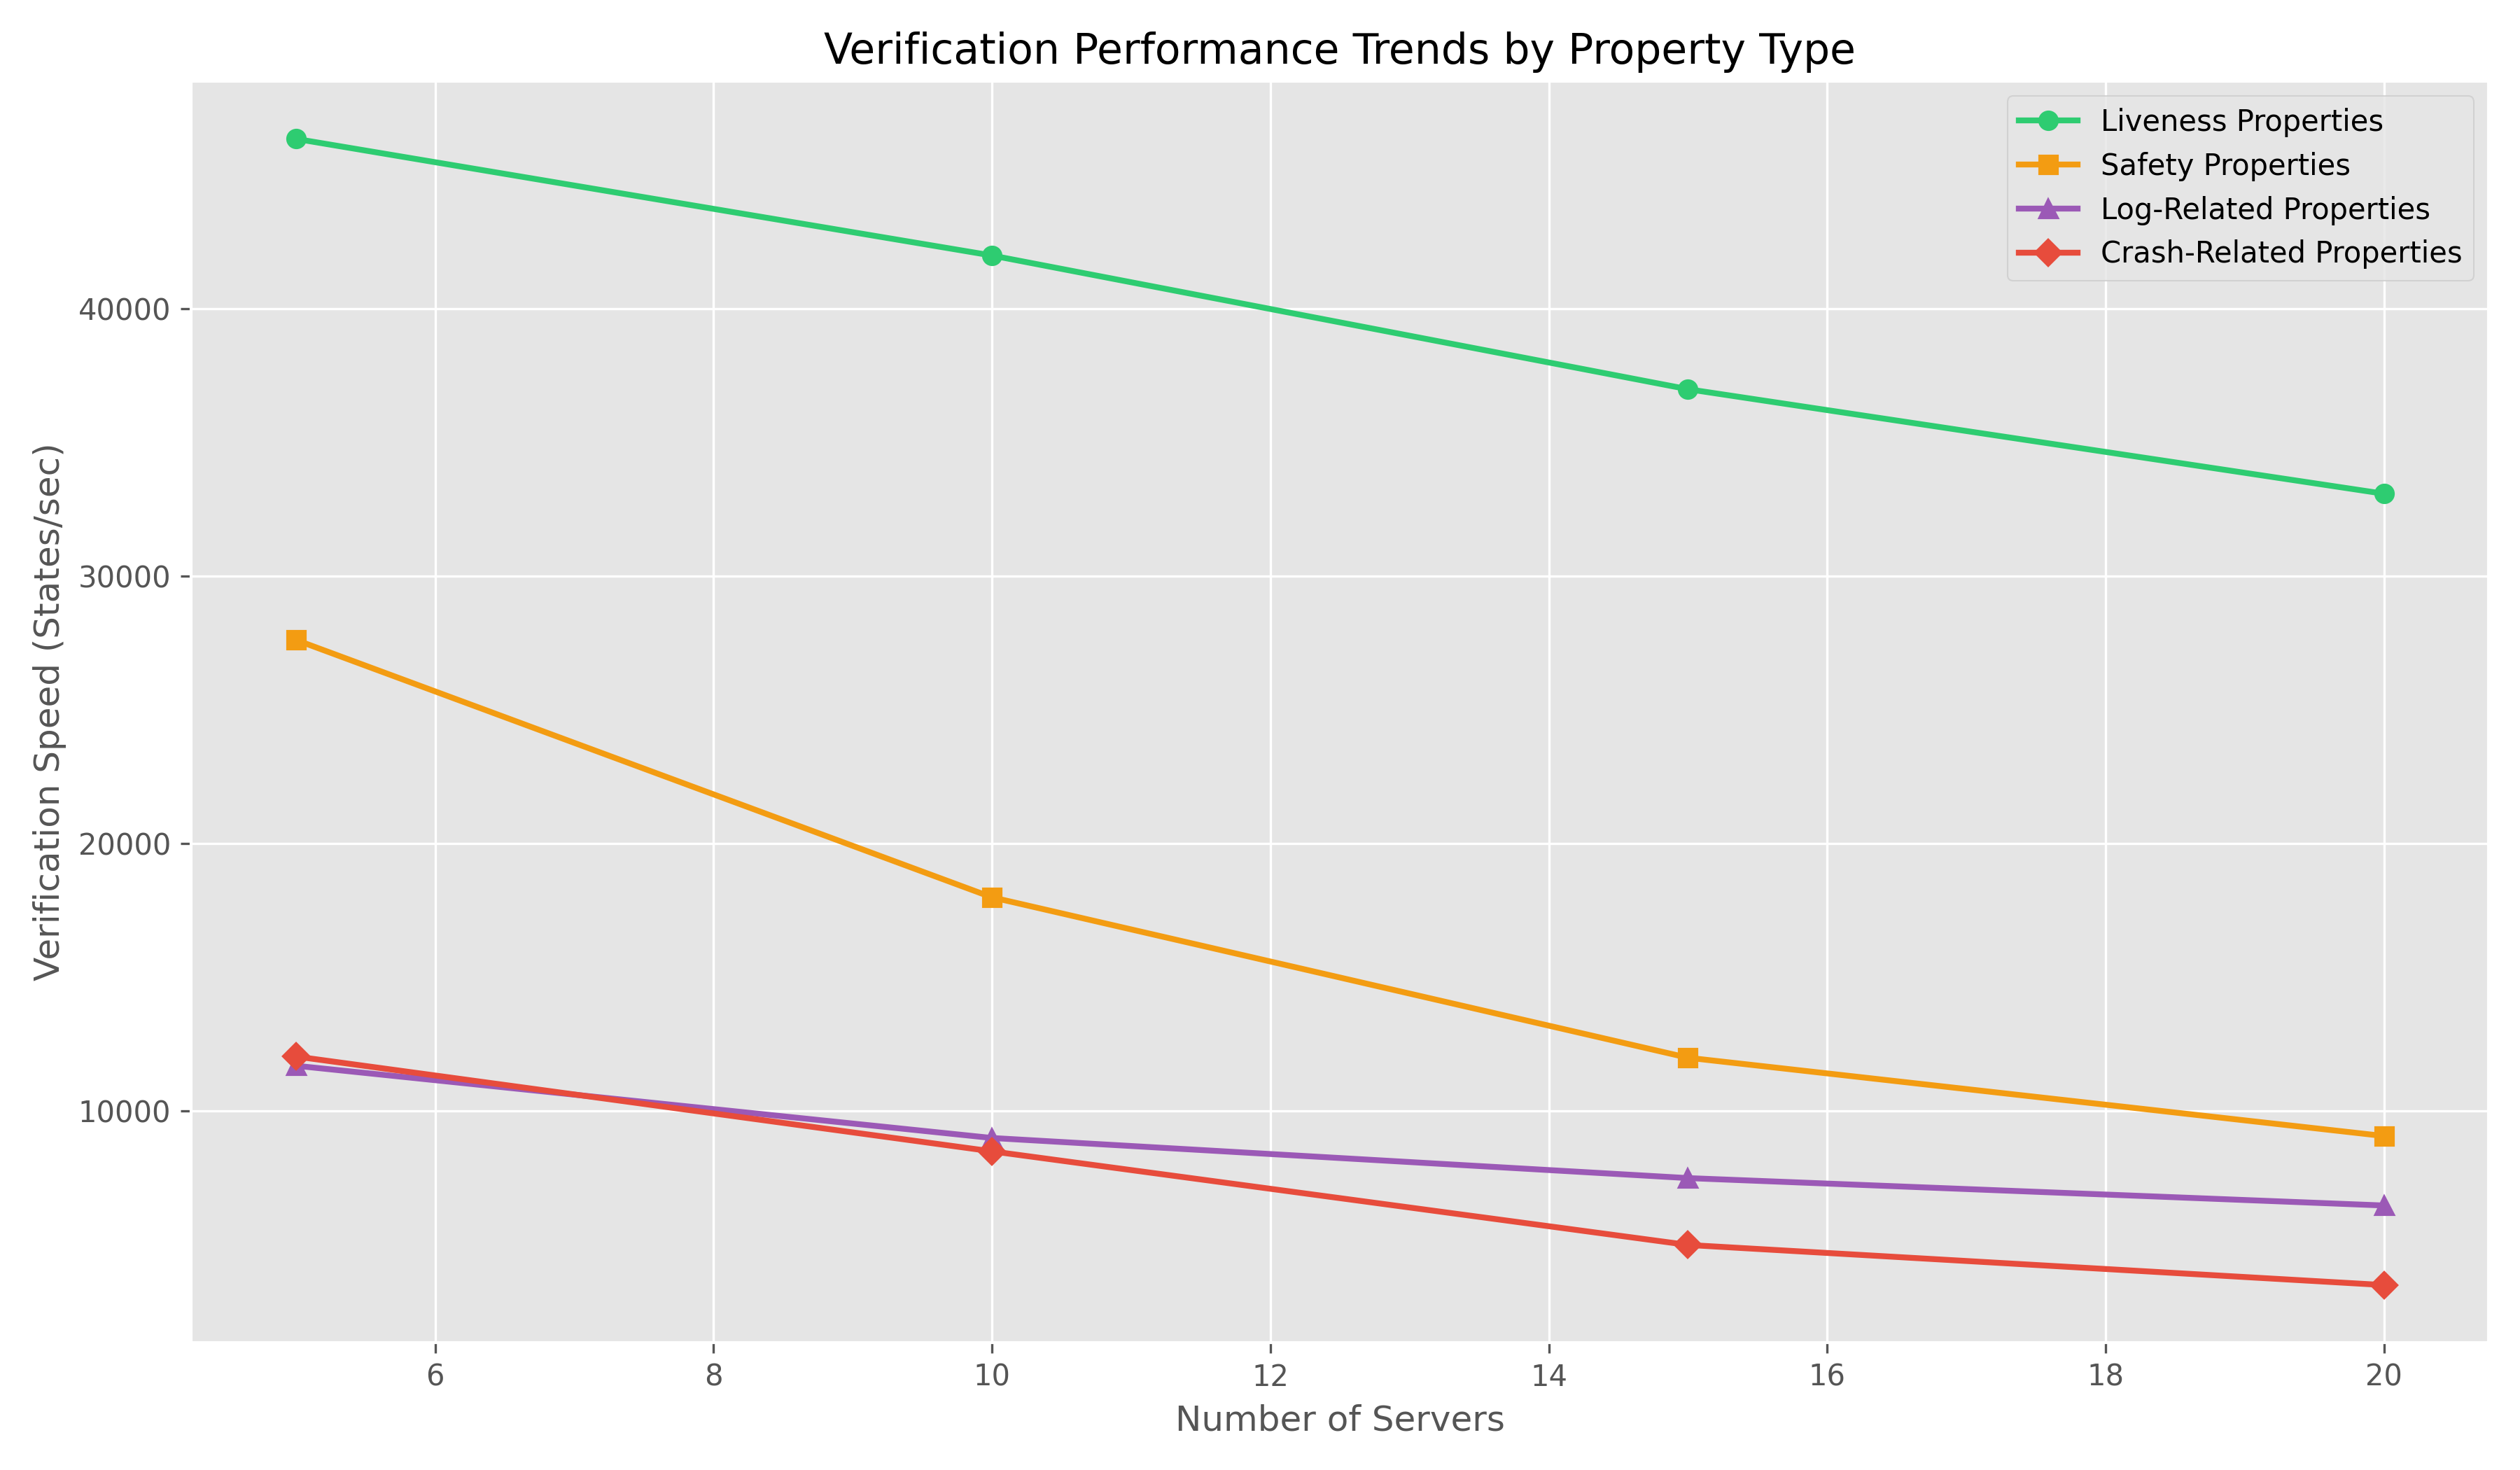
\includegraphics[width=0.95\textwidth]{graphs/performance_trends.png}
    \caption{Verification speed trends across server configurations by property type. Liveness properties consistently outperform other property types, while crash-related properties show the steepest performance decline.}
    \label{fig:performance-trends}
\end{figure}

This visualization clearly demonstrates the divergent scaling behaviors: liveness properties maintain relatively high verification speeds even at 20 servers, while crash-related properties experience a much steeper decline. This insight suggests that different optimization strategies should be applied based on the type of property being verified.

\subsection{Implications for Verification Strategy}

These graphical analyses highlight the need for property-specific verification approaches when analyzing complex distributed systems like the Raft consensus algorithm. While all properties were successfully verified without finding safety violations, the performance characteristics suggest that:

\begin{itemize}
    \item Liveness properties can be efficiently verified even for larger configurations
    \item Crash-related properties may benefit from specialized state space reduction techniques
    \item Memory consumption scales predictably, allowing for resource planning
    \item Future verification efforts should consider property-specific optimization strategies
\end{itemize}

The consistent performance patterns across server configurations provide confidence that our verification approach can be extended to even larger systems with appropriate computational resources. 